%!TEX root = fundamentos.tex
\chapter{Conjuntos, Rela\coes e Fun\coes}

\section{Conjuntos}\label{conjuntos}

A teoria dos conjuntos forma a base de quase toda a matem\'atica. Surpreendentemente, seu desenvolvimento \'e relaticamente recente, tendo come\cc ado com Georg Cantor, uma matem\'atico alem\aoi, no s\'eculo XIX (para uma breve hist\'oria do assunto verifique \cite{johnson:1972}). A pr\ih ncipio a teoria de conjuntos parece ser bem simples, mas alguns dos problema que surgem desta teoria s\ao bem s\'utis. Estes problemas s\ao ainda objetos de estudo e debate entre matem\'aticos e este estudo nos leva a um entendimento mais profundo dos fundamentos da matem\'atica. Assim, a teoria dos conjuntos se tornou uma das mais frut\ih feras ideias em toda a matem\'atica.

Embora seja poss\ih vel desenvolver a teoria dos conjuntos de um ponto de vista axiom\'atico, uma abordagem informal ser\'a mais adequada para nosso prop\'ositos (\cite{halmos:1974} fornece uma introdu\caoi, relativamente f\'acil de ler, para um desenvolvimento axiom\'atico). Para come\cc ar, podemos pensar em um conjunto como Cantor fez, como ``uma cole\cao objetos distingu\ih vies, chamados elementos, pensado como um todo.'' Obviamente, isto n\ao serve como uma defini\cao para conjunto a menos que cole\cao tenha sido definida proviamente e facilmente vemos que estamos presos em um padr\ao circular de defini\cois. De fato, em qualquer l\ih ngua existem termos que s\ao indefinidos dentro daquela l\ih ngua. Isto tamb\'em \'e verdade em mate\'atica e tomaremos conjunto e elemento de um conjunto para serem primitivos, termos indefinidos.

Do ponto de vista intuitivo pareceria que qualquer cole\cao de objetos podeira ser considerada como um conjunto (certamente, na considera\cao de Cantor isso procedia), entretanto, este n\ao \'e o caso. Nos fins do s\'eculo XIX matem\'aticos descobriram que permitindo uma cole\cao ser um conjunto levou a paradoxos l\'ogicos de todas as formas. Duas formas principais foram descobertos para eliminar este paradoxo; conjuntos n\ao foiram permitidos para ser ``muito grande'' ou restri\coes foram  colocadas sobre a esp\'ecie que poderiam ser elementos dos conjuntos (para um discuss\ao interessante das quest\oes envolvidas, veja \cite{pinter:1971}). Estas dificuldades n\ao precisam nos preocupar aqui, mas faremos a premissa que todos os conjuntos em discuss\ao consistem de elementos de um conjunto universal, usualmente denotado por $\mathbb{U}$. Muito frequentemente $\mathbb{U}$ n\ao ser\'a  mencionado explicitamente, logo esta situa\cao \'e muito similar a ideia de dom\ih nio da uma vari\'avel para uma fun\cao proposicional. Assim, quando escrevemos $\forall a, a \textrm{ em } A\to a \textrm{ em } B,$ estamos realmente querendo dizer $\forall a\in\mathbb{U}, a \textrm{ em } A\to a \textrm{ em } B,$ para algum conjunto universal $\mathbb{U}$. 

Denotaremos usualmente comjuntos por letras mai\'usculas $A$, $B$, $C$, etc. Os elementos dos conjuntos ser\ao representados por lebras min\'usculas $a$, $b$, $c$, etc. ``$a$ \'e um elemento do conjunto $A$'' ou ``$a$ \'e um membro de $A$'' ou ``$a$ pertence a $A$'' \'e denotado por
\[
a\in A
\]
e ``$a$ n\ao \'e um elemento do conjunto $A$'' por
\[
a\notin A.
\]
Se um conjunto n\ao tem muitos elementos, \'e conveniente list\'a-los, entre par\^enteses: $\{\ldots\}$. Assim, de $A$ \'e um conjunto com elementos $1,2,3,4$, indicaremos isto por
\[
A=\{1,2,3,4\}.
\]
Outra forma de especificar os elementos de um conjunto \'e dar a regra de forma\cao dos membro do conjunto. Portanto, se $A$ \'e como acima, poder\ih amos tamb\'em indicar este conjunto por
\begin{eqnarray*}
& A = \{a: a \textrm{ \'e um inteiro e } 1\leq a \leq 4\} \textrm{ ou }\\
& A = \{x: (x-2)(x-1)(x-4)(x-3)=0\}.
\end{eqnarray*}
A nota\cao $\{a:p(a)\}$ \'e lida como ``o conjunto de todos $a$ tais que $p(a)$ \'e verdade'' (aqui $p$ \'e alguma fun\cao proposiciponal). Este conjunto pode ser escrito tamb\'em como $\{a|p(a)\}$. No que, a ordem na qual os elementos de um conjunto s\ao listados n\ao fazem diferen\cc a, pelo simple caso que se a odem fosse importante ent\ao o m\'etodo de especificar os elementos de um conjunto  por uma regra de forma\cao n\ao funcionaria, para tal especifica\cao n\ao implica necessariamente uma ordem particular.

O leitor mais alerta pode ter notado que j\'a usamos igualdade de conjuntos sem mencionar qual \'e o significado de ``conjunto $A$ \'e igual ao conjunto $B$.'' Para solucionar esta defici\^encia, definamos o seguinte:

\begin{definb}
O conjunto $A$ \'e {\it igual}\index{Conjuntos!Igualdade} ao conjunto $B$, denotado por $A=B$, se e somente se todo elemento de $A$ \'e um elemento de $B$ e todo elemento de $B$ \'e um elemento de $A$. Em s\ih mbolos,
\begin{eqnarray*}
&(A=B)\leftrightarrow [(\forall x, x\in A \to x\in B)\ee(\forall x, x\in B \to x\in A)] \textrm{ ou } \\
&(A=B)\leftrightarrow (\forall x, x\in A \leftrightarrow x\in B).
\end{eqnarray*}
\end{definb}
 
Assim dois conjuntos s\ao iguais se e somente se eles t\^em os mesmos elementos, por exemplo,
\[
\{1,2,3\}=\{2,3,1\}=\{x|a\leq x\leq 3 \textrm{ e $x$ \'e um inteiro.}\}.
\]

Existem muitos conjuntos que s\ao frequentemente usados em matem\'atica, por isso damos a eles nomes especiais. Talvez este conjuntos s\ao familiares a voc\^e:
\begin{eqnarray*}
\mathbb{N}&=&\{x|\espaco x \textrm{ \'e um inteiro e $x\geq 1$}\}=\{1,2,3,4\ldots\} \textrm{ {\bf (conjunto dos n\'umeros naturais)}}\\
\mathbb{Z}&=&\{x|\espaco x \textrm{ \'e um inteiro}\}=\{\ldots,-2,-1,0,1,2,\ldots\} \textrm{ {\bf (conjunto dos n\'umeros inteiros)}}\\
\mathbb{Q}&=&\left\{\dfrac{x}{y}: \espaco x,y\in\mathbb{Z},y\neq 0\right\}=\left\{\ldots,\dfrac{-4}{3},\dfrac{-3}{2},\dfrac{-2}{1},\dfrac{-1}{1},\dfrac{0}{2},\dfrac{1}{3},\dfrac{2}{4},\ldots\right\} \textrm{ {\bf (conjunto dos n\'umeros racionais)}}\\
\mathbb{R}&=&\{x|\espaco \textrm{ \'e um n\'umero real}\} \textrm{ {\bf (conjunto dos n\'umeros reais)}}
\end{eqnarray*}
Suponha que $A=\{1,2,3\}$ e $B=\{1,2,3,4\}$. Facilmente vemos que $A\neq B$ ($4\in B$ mas $4\notin A$) mas podemos ver que todos os elementos de $A$ s\ao tamb\'em elementos de $B$. Isto \'e um importante conceito, por isso daremos um nome:

\begin{definb}
Sejam $A,B$ conjuntos. Dizemos que $A$ \'e um {\it subconjunto}\index{Subconjunto}  de $B$ (ou equivalentemente, $B$ \'e um superconjunto de $A$) se e somente se, todos elementos de $A$ s\ao um elemento de $B$. Isto \'e denotado por
\[
A \subseteq B \textrm{ ou } B \supseteq A. 
\]
\end{definb}

Em s\ih mbolos,
\[
A \subseteq B \leftrightarrow (\forall x,\espaco x\in A \to x\in B).
\]
Se $A$ n\ao \'e um subconjunto de $B$, escreveremos $A\not\subseteq B$. Aplicando nossas t\'ecnicas para nega\cao de fun\coes proposicionais quantificadas obtemos:
\[
A\not\subseteq B \leftrightarrow \nao(\forall x,\espaco x\in A \to x\in B) \leftrightarrow (\exists x \ni \espaco x\in A \to x\notin B).
\]
Note que, para qualquer conjunto $A$, \'e verdade que $A \subseteq A$. Se $A \subseteq B$ mas $A\neq B$ ent\ao diremos que $A$ \'e um {\it subconjunto pr\'oprio}\index{Subconjunto Pr\'oprio} de $B$ e escrevemos
\[
A\subset B \textrm{ ou } B\supset A.
\] 
De forma similar, se $A$ n\ao \'e um subconjunto pr\'oprio de $B$ escreveremos $A\not\subset B$. [Note que, alguns autores n\ao fazem uma distin\cao e usam $\subset$ como usamos $\subseteq$ e assim n\ao tem um s\ih mbolo distinto para subconjuntos pr\'oprios].

Como exemplos desta nota\caoi, se $A=\{1,2,3,4\}$, $B= \{x: (x-2)(x-1)(x-4)(x-3)=0\}$ e $C=\{1,2,3,4,5,6\}$ ent\ao
\[
A\subseteq B, \espaco B\subseteq C, \espaco C\subseteq \mathbb{N}
\]
e
\[
A\not\subset B, \espaco B\subset C, \espaco C\subset \mathbb{N}.
\]

Permitindo que um conjunto seja uma cola\cao de objetos, obviamente \'e poss\ih vel ter uma cole\cao sem objetos, poe exemplo, o conjunto de todos os estudantes de matem\'atica que tem mais de seis metros de altura. Chamamos um conjunto se elementos de {\it conjunto vazio}.\index{Conjuntos!Vazio} Se tivermos dois conjuntos, digamos, o conjunto descrito acima e o conjunto de todos os professores de matem\'atica que t\^em menos de seis milimetros de altura. Podemos ver que estes conjuntos s\ao iguais desde que ambos satisfazem a defini\cao de igualdade de conjuntos. Assim, como quaisquer dois conjuntos como os acima s\ao iguais, ent\ao existe apenas um conjunto vazio com isso podemos dizer o conjunto vazio que \'e representado, $\varnothing$ e em s\ih mbolos por
\[
\varnothing = \{x| \espaco p(x)\ee \nao p(x)\},
\]  
onde $p$ \'e qualquer fun\cao proposicional.

Como ``$\forall x\in D,\espaco x\in\varnothing$'' \'e falso se $D$ \'e n\ao vazio, ``$\forall x\in D,\espaco x\in\varnothing\to \textrm{(qualquer fun\cao proposicional)}$'' \'e verdade (\`as vezes dizemos que tal implica\cao \'e verdade por vacuidade pois a premissa nunca \'e verdade) portanto em particular
\[
\forall x, \espaco x\in\varnothing\to x\in A
\] 
\'e verdade para qualquer conjunto $A$, temos que $\varnothing\subseteq A.$

Se voc\^e estiver um pouco confuso, pode ser poss\ih vel confundir as ideias de elementos (regra de forma\caoi) e subconjunto. Para manter estas ideias distintas, lembre que ``\'e um subconjunto de'' \'e uma rela\cao que existe (ou n\aoi) entre conjuntos, enquanto ``ser membro de'', isto \'e ``\'e um elemento de,'' \'e uma rela\cao que existe (ou n\aoi) elementos e conjuntos. Assim,, para uma sente\cc a envolvendo $\subseteq$ para fazer sentido deve ter conjuntos em ambos os lados de $\subseteq$, enquanto um elemento deve estar a esquerda de $\in$ e um conjunto que contenha elementos deste tipo a direita. Por exemplo, todas a proposi\coes abaixo s\ao verdade:
\[
1\in\{1,2\},\espaco 1\not\subseteq\{1,2\},\espaco \{1\}\subseteq\{1,2\},\espaco \varnothing\notin\{1,2\},\espaco \varnothing\subseteq\{1,2\}  
\]  
enquanto as seguintes s\ao falsas:
\[
1\subseteq\{1,2\},\espaco 1\notin\{1,2\},\espaco \{1\}\in\{1,2\},\espaco \varnothing\in \{1,2\}.
\]
Seguindo este padr\ao de l\'ogica onde combinamos proposi\coes usando conectivos para obter novas proposi\cois, desejamos combinar conjuntos para obter novos conjuntos usando o que chamaremos de {\it opera\coes de conjuntos}.\index{Conjuntos!Opera\cois} Suas defini\coes s\ao

\begin{definb}
Sejam $A,B$ conjuntos. Ent\ao a {\it uni\ao}\index{Conjuntos!Uni\aoi} de $A$ e $B$ (denotada por $A\cup B$) \'e o conjunto de todos os elementos que est\ao pelo menos um de $A$ ou $B$. Em s\ih mbolos, 
\[
A \cup B = \{x:x\in A \ou x\in B\}. 
\]
A {\it intersec\cao}\index{Conjuntos!Intersec\caoi} de $A$ e $B$ (denotada por $A\cap B$) \'e o conjunto de todos os elementos que est\ao em ambos $A$ e $B$. Em s\ih mbolos, 
\[
A \cap B = \{x:x\in A \ee x\in B\}. 
\]
Se $A\cap B=\varnothing,$ dizemos que $A$ e $B$ s\ao {\it disjuntos}\index{Conjuntos!Disjuntos}. O {\it complemento relativo}\index{Conjuntos!Complemento Relativo} de $A$ em $B$ (ou complemento de $A$ com respeito a $B$), denotado por $B-A$ (\`as vezes por $B \backslash A$) \'e o conjunto de todos os elementos em $B$ que n\ao est\ao em $A$. Em s\ih mbolos,
\[
B-A = \{x:x\in B \ee x\notin A\}. 
\]
Se $B$ \'e $\mathbb{U}$, o conjunto universal, ent\ao $\mathbb{U}-A = \{x:x\in \mathbb{U} \ee x\notin A\}=\{x:x\notin A\}$ \'e chamado o {\it complemento}\index{Conjuntos!Complemento} de $A$ e \'e denotado por $A^{C}$.
\end{definb}

Uma forma conveniente de exibir conjuntos \'e tendo uma imagem visual de uni\ois, intersec\coes e complementos relativos. Para isso usamos um {\it diagrama de Venn}\index{Diagrama de Venn} (veja os exemplos abaixo). Para este tipo de diagramas usamos regi\oes para representar conjuntos a regi\ao cercada por um ret\^angulo representa o conjunto universal e as regi\oes dentro de c\ih rculos representam os conjuntos indicados (e portanto a regi\ao fora do c\ih rculo $A$ representa $A^C$). Assim, aregi\ao compartilhada por dois c\ih rculos representa $A\cap B$ (sombreada no seguinte diagrama):

%%%%%%%%%%%%%%%%%%%%%diagrama de Venn (A inter B)%%%%%%%%%%%%%%%%%%%%%%%%%%%%%%%%%%
\def\rectangle{(-3,-2) rectangle (5,2)}
\def\firstcircle{(0,0) circle (1.5cm)}
\def\secondcircle{(60:2cm) circle (1.5cm)}
\def\thirdcircle{(0:2cm) circle (1.5cm)}
\begin{figure}[h]
\centering
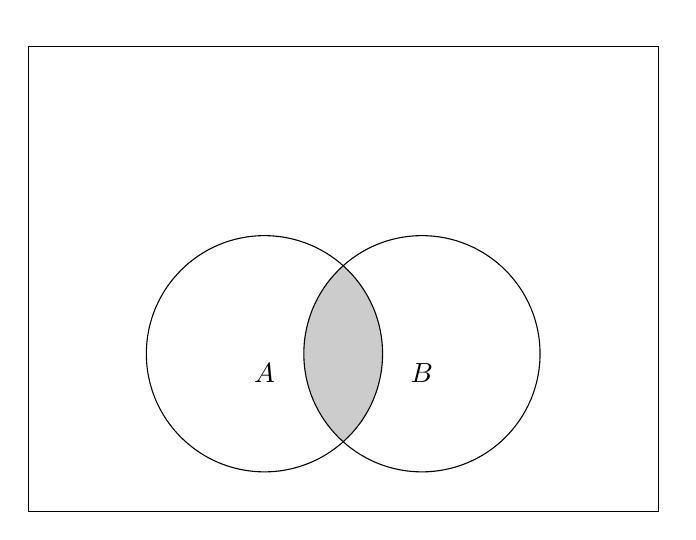
\begin{tikzpicture}
    \begin{scope}[shift={(10cm,10cm)}, fill opacity=0.5]
        \fill[white] \rectangle;
        \clip \firstcircle;
        \fill[gray!40] \thirdcircle;
    \end{scope}
    \begin{scope}[shift={(10cm,10cm)}, fill opacity=1.0]
        \fill[white] \rectangle;
        \clip \thirdcircle;
        \fill[gray!40] \firstcircle;
    \end{scope}
    \begin{scope}[shift={(10cm,10cm)}]
        \draw \rectangle node[text=black,above] {};
        \draw \firstcircle node[text=black,below] {$A$};
        \draw \thirdcircle node [text=black,below] {$B$};
    \end{scope}
\end{tikzpicture}
\\
$A\cap B$
\end{figure}
%%%%%%%%%%%%%%%%%%%%%%%%%%%%%%%%%%%%%%%%%%%%%%%%%%%%%%%%%%%%%%%%%%%%%%%%%%%%%%%%%%%%
enquanto as duas regi\oes para $A$ e $B$ tomadas juntas representam $A\cup B$

%%%%%%%%%%%%%%%%%%%%%diagrama de Venn (A union B)%%%%%%%%%%%%%%%%%%%%%%%%%%%%%%%%%%
\def\rectangle{(-3,-2) rectangle (5,2)}
\def\firstcircle{(0,0) circle (1.5cm)}
\def\secondcircle{(60:2cm) circle (1.5cm)}
\def\thirdcircle{(0:2cm) circle (1.5cm)}
\begin{figure}[h]
\centering
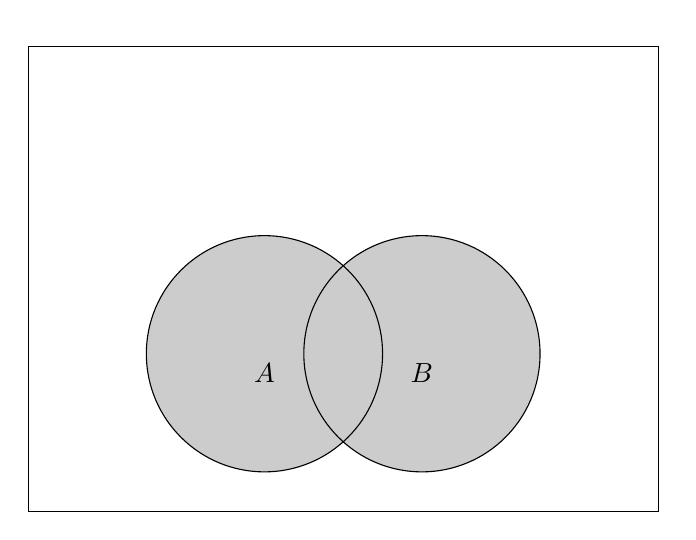
\begin{tikzpicture}
    \begin{scope}[shift={(10cm,10cm)}, fill opacity=1.0]
        \fill[white] \rectangle;
        \fill[gray!40] \firstcircle;
        \fill[gray!40] \thirdcircle;
    \end{scope}
    \begin{scope}[shift={(10cm,10cm)}]
        \draw \rectangle node[text=black,above] {};
        \draw \firstcircle node[text=black,below] {$A$};
        \draw \thirdcircle node [text=black,below] {$B$};
    \end{scope}
\end{tikzpicture}
\\
$A\cup B$
\end{figure}
%%%%%%%%%%%%%%%%%%%%%%%%%%%%%%%%%%%%%%%%%%%%%%%%%%%%%%%%%%%%%%%%%%%%%%%%%%%%%%%%%%%%
e a regi\ao sombreada abaixo representa $A-B$

%%%%%%%%%%%%%%%%%%%%%diagrama de Venn (A-B)%%%%%%%%%%%%%%%%%%%%%%%%%%%%%%%%%%
\def\rectangle{(-3,-2) rectangle (5,2)}
\def\firstcircle{(0,0) circle (1.5cm)}
\def\secondcircle{(60:2cm) circle (1.5cm)}
\def\thirdcircle{(0:2cm) circle (1.5cm)}
\begin{figure}[h]
\centering
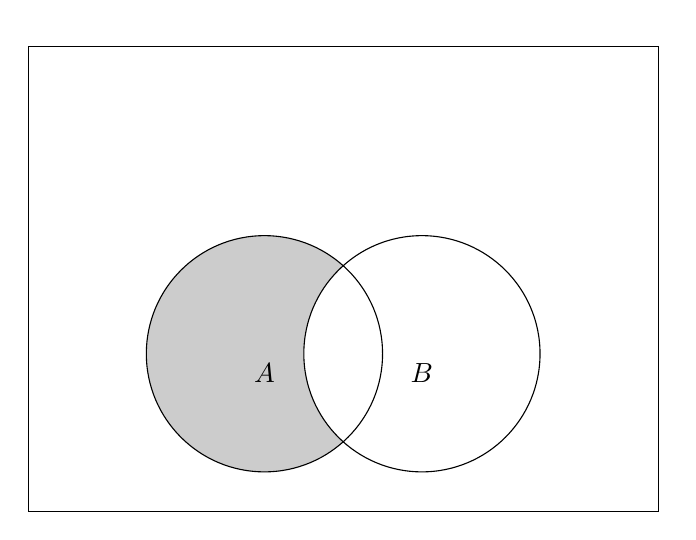
\begin{tikzpicture}
        \begin{scope}[even odd rule]% first circle without the second
        \clip \thirdcircle (-3,-2) rectangle (5,2);
        \fill[gray!40] \firstcircle;
        \end{scope}
        \draw \rectangle node[text=black,above] {};
        \draw \firstcircle node[text=black,below] {$A$};
        \draw \thirdcircle node [text=black,below] {$B$};
\end{tikzpicture}
\\
$A - B$
\end{figure}
%%%%%%%%%%%%%%%%%%%%%%%%%%%%%%%%%%%%%%%%%%%%%%%%%%%%%%%%%%%%%%%%%%%%%%%%%%%%%%%%%%%%
O mesmo princ\ih pio pode ser usado quando temos tr\^es conjuntos envolvidos, por exemplo (o leitor deve verificar este fato), a regi\ao sombreada abaixo representa $(A\cap C)\cup(B\cap C)$:

%%%%%%%%%%%%%%%%%%%%%diagrama de Venn ((A inter C) union (B inter C))%%%%%%%%%%%%%%%
\def\rectangle{(-3,-2) rectangle (5,3.9)}
\def\firstcircle{(0,0) circle (1.5cm)}
\def\secondcircle{(60:2cm) circle (1.5cm)}
\def\thirdcircle{(0:2cm) circle (1.5cm)}
\begin{figure}[h]
\centering
    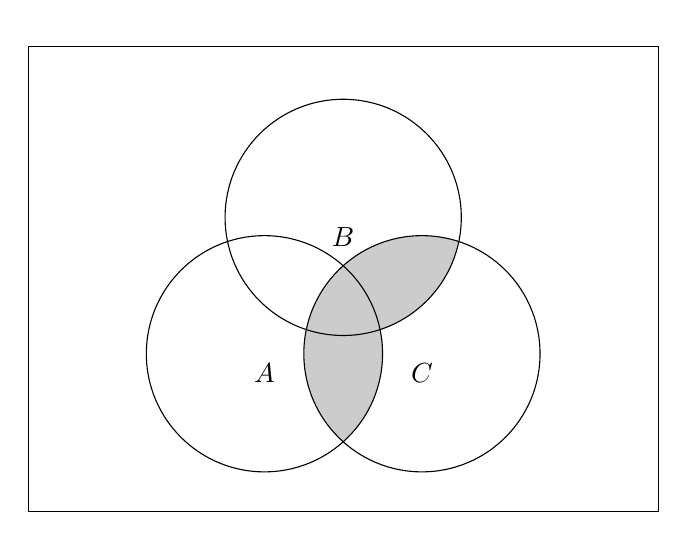
\begin{tikzpicture}
      \begin{scope}
    \clip \secondcircle;
    \fill[gray!40] \thirdcircle;
      \end{scope}
      \begin{scope}
    \clip \firstcircle;
    \fill[gray!40] \thirdcircle;
      \end{scope}
      \draw \rectangle node[text=black,above] {};
      \draw \firstcircle node[text=black,below] {$A$};
      \draw \secondcircle node [text=black,below] {$B$};
      \draw \thirdcircle node [text=black,below] {$C$};
    \end{tikzpicture}
\\
$(A\cap C)\cup(B\cap C)$
\end{figure}
%%%%%%%%%%%%%%%%%%%%%%%%%%%%%%%%%%%%%%%%%%%%%%%%%%%%%%%%%%%%%%%%%%%%%%%%%%%%%%%%%%%%
Note que quando t\ih nhamos dois conjuntos o diagrama de Venn consistia de quatro regi\oes enquanto que quando t\ih nhamos tr\^es conjuntos existiam oito regi\ois. Com um pouco mais de trabalho podemos mostrar porque este \'e o caso: para um elemento em $\mathbb{U}$ e cada conjunto envolvido, exatamente uma de duas possibilidades devem ocorrer: o elemento pertence ou n\ao pertence ao conjunto. Assim com dois conjuntos temos $2\times 2=4$ possibilidades enquanto que para tr\^es conjuntos temos $2\times 2\times 2=8$ possibilidades. Voc\^e provavelmente nunca viu um diagrama de Venn com seis conjuntos, tal diagrama teria $2^6=64$ regi\oes e sua complexidade faria que sua utilidade fosse limitada.

Existe um outro conjunto obtido de um conjunto dado o qual chamamos de chamamos de o {\it conjunto de todos os subconjuntos de um conjunto dado.}

\begin{definb}
Seja $A$ um conjunto. Ent\ao o conjunto de todos os subconjuntos de $A$, denotado por $\mathbb{P}(A)$ (ou $2^{A}$) \'e chamado de o {\it conjunto pot\^encia}\index{Conjuntos!Conjunto Pot\^encia} de $A$. Em s\ih mbolos, 
\[
\mathbb{P}(A) = \{B:B\subseteq A\}. 
\]
\end{definb}
Para ter certeza que estas ideias est\ao claras, vamos considerar alguns exemplos.

Seja $\mathbb{U}$ o conjunto dos n\'umeros naturais (usualmente denotado por $\mathbb{N}$), isto \'e,
\[
\mathbb{U}=\mathbb{N}=\{x|\espaco x \textrm{ \'e um inteiro e $x\geq 1$}\}=\{1,2,3,4\ldots\}
\]
Definimos
\begin{eqnarray*}
A&=&\{x:\espaco x \textrm{ \'e par}\},\\
B&=&\{x:\espaco x=2k-1 \textrm{ para algum } k\in\mathbb{N}\},\\
C&=&\{y:\espaco y\leq 4\},\\
D&=&\{1,3\}.\\
\end{eqnarray*}
Portanto (o leitor deve verificar):
\begin{eqnarray*}
&& A\cup B = \mathbb{U},\\
&& A\cap B = \varnothing,\\
&& \textrm{$A$ e $D$ s\ao disjuntos,}\\
&& A^C=B,\\
&& B^C=A,\\
&& A-B=A,\\
&& C\cap D=D,\\
&& \mathbb{P}(D)=\{\varnothing,\{1\},\{3\},\{1,3\}\},\\
&& C\not\subseteq D,\\
&& D-C=\varnothing,\\
&& D\subseteq C,\\
&& D\subset C,\\
&& D^C\supseteq A,\\
&& 1\not\subseteq D,\\
&& 1\in D,\\
&& A\cup C=A\cup D,\\
&& \varnothing\in \mathbb{P}(D),\\
&& \varnothing\subseteq\mathbb{P}(D),\\
&& \{1\}\in\mathbb{P}(D),\\
&& 1\notin\mathbb{P}(D).
\end{eqnarray*}

Vamos provar alguns teoremas envolvendo conjuntos, mas primeiro ser\'a \'util fazer algumas observa\coes sobre tais demonstra\cois. Um dos tipos mais comuns de demonstra\cao \'e a demonstra\cao direta para mostrar que um conjunto \'e um subconjunto de outro conjunto. Apresentamos um exemplo espec\ih fico:
\\
\\
{\bf Teorema:} Sejam $A$ e $B$ conjuntos tais que $A\cap B=A$. Ent\ao $A\subseteq B.$
\\
\\
\begin{proof} 
Suponha que $A,B$ s\ao conjuntos tais que $A\cap B=A$. Seja $a\in A.$ Ent\aoi,
\\
\ldots
\\ 
``alguma coisa utilizando a hip\'otese  $A\cap B=A$''
\\
\ldots
\\
portanto, $a\in B$. Assim $A\subseteq B.$
\end{proof}
\\ 

Alguns coment\'arios sobre esta demonstra\cao est\ao em ordem. Note que come\cc amos a demonstra\cao por ``preparando o terreno'', isto \'e definimos o que nossos s\ih mbolos representam e que hip\'oteses foram feitas sobre eles. Esta \'e uma boa form para come\cc ar qualquer demonstra\caoi, embora voc\^e pode ter notado que em livros texto de matatem\'atica, especialmente os mais avan\cc ados, geralmente omitem isso e assumem que o leitor pode inferir do contexto que os s\ih mbolos representam e que premissas est\ao sendo feitas sobre eles. Isto mostra um aspecto da escrita de demonstra\coes que requer o julgamento: quantos detalhes devem ser incluidos. N\ao existe uma resposta correta para esta pergunta, mas uma boa pr\'atica \'e incluir os detalhes suficientes para que a pessoa com um n\ih vel entendimento mais baixo dentro dos universo dos poss\ih veis leitores seja capaz de compreender a demonstra\caoi. Quando estamos come\cc ando devemos ter como objetivo para o detalhe suficiente de tal forma que possamos entender nossa pr\'opria demonstra\cao na semana seguinte, isto \'e depois que algum tempo tenha passado e as ideias da demonstra\cao n\ao estejam t\ao claras em nossa mente. Na d\'uvida, erre no exagero, ou seja, abuse dos detalhes.

Depois que ``preparamos o terreno,'' a demonstra\cao come\cc ou. ``Seja $a\in A$.'' Este \'e outro exemplo do uso de uma vrai\'vel ``fixa mas arbritr\'aria.'' Assumimos que $a$ \'e um elemento de $A$, nada mais que isso \'e assumido. Mas, espere! H\'a mais do que foi dito. Estamos aqui, de fato, considerando dois casos, um que nem \'e mesmo mencionado. Quando dizemos ``seja $a\in A$,'' estamos assumindo que $A\neq\varnothing$. E se tiv\'essemos $A=\varnothing$? Este \'e o caso n\ao mencionado que ficou impl\ih cito. A raz\ao para n\ao mencionar este caso \'e que se $A=\varnothing$, a demonstra\cao estar\'a completa, pois $\varnothing$ \'e subconjunto de qualquer conjunto, em particular $B$. Uma forma mais geral de pensar nisso \'e perceber que a proposi\cao que estamos tentando demonstrar ($\forall x, \espaco x\in A\to x\in B $) \'e uma implica\cao universalmente quantificada. Se n\ao h\'a elementos em $A$, a implica\cao \'e verdade por vacuidade. Se fossemos escrever isto em detalhes (que usualmente n\ao \'e feito), come\cc ar\ih amos com: ``Consideremos dois casos: $A=\varnothing$ e $A\neq\varnothing$. Se $A=\varnothing$ ent\ao $A\subseteq B$ e a demonstra]\cao estar\'a terminada. Se $A\neq\varnothing$, seja $a\in A$ \ldots'' O ponto para lembrar \'e que sempre que escrevemos alguma coisa como ``seja $a\in A$,'' devemos ter claro que o caso $A=\varnothing$ n\ao causa nenhum problema. Outro ponto importante para notar \'e que devemos mostrar que a conclus\ao do teorema ($A\subseteq B$ ou $\forall x, \espaco x\in A\to x\in B$) \'e verdade, nossa escolha do elemento ``fixo mas arbitr\'ario'' \'e determinado pela conclus\ao ao inv\'es das hip\'oteses (que neste caso \'e $A\inter B=A$). Mais geralmente o ``alguma coisa ou outra'' no corpo da demonstra\cao vem a ser apenas uma tradu\cao das defini\cois, por exemplo,  $x\in A\inter B$ implica que $x\in A$ e $x\in B$. O ``$\Box$'' ao fim da demonstra\cao \'e um s\ih mbolo para indicar que demonstra\cao est\'a completa.

Podemos usar esta mesma t\'ecnica duas vezes para mostrar que dois conjuntos s\ao iguais, isto \'e $A=B$ se e somente se $A\subseteq B$ e $B\subseteq A$. Portanto, para mostrar que $A=B$, mostramos que $A\subseteq B$ e ent\ao demonstramos que $B\subseteq A$. Como exemplo deste tipo de demonstra\cao considere:

\begin{teob}
Sejam $A$ e $B$ conjuntos. Ent\ao $A-B=A\cap B^C.$
\end{teob}
\begin{proof} Suponha que $A$ e $B$ sejam conjuntos. Primeiro, mostremos que $A-B\subseteq A\inter B^C$. Seja $x \in A-B$. Ent\ao $x\in A$ e $x\notin B$ (esta \'e apenas a defini\cao de $A-B$). Mas $x\notin B$ implica que $x\in B^C$. Portanto, $x\in A$ e $x\in B^C$ assim temos que $x\in A\inter B^C$ e $A-B\subseteq A\inter B^C$.

Agora, suponha que $X\in A\inter B^C$. Isto significa que $x\in A$ e $x\in B^C$ (novamente, usando a defini\cao do conjunto em quest\aoi, neste caso a intersec\caoi). Mas $x\in B^C$ significa que $x\notin B$. Portanto, $x\in A$ e $x\notin B$, ou seja, $X\in A-B$, logo $A\inter B^C\subseteq A-B$.

Como mostramos que $A-B\subseteq A\inter B^C$ e $A\inter B^C\subseteq A-B$, demonstramos que $A-B= A\inter B^C$. 
\end{proof}
\\

Inclu\ih mos aqui uma demostra\cao mais detalhada que o normal pois esta \'e a nossa primeira demonstra\cao de um teorema. Usualmente os lembretes entre par\^enteses n\ao apareceriam no corpo da demonstra\cao e menos explica\cao seria dada.

Abaixo est\'a outro exemplo, com um pouco menos de explica\caoi:

\begin{teob}
Sejam $A$, $B$ e $C$ conjuntos com $A\subseteq B$ e $B\subseteq C$. Ent\ao $A\subseteq C.$
\end{teob}
\begin{proof} 
Suponha que $A$, $B$ e $C$ sejam conjuntos com $A\subseteq B$ e $B\subseteq C$. Seja $x\in A$. Ent\ao como $A\subseteq B$ temos que $a\in B$. Al\'em disso, como $B\subseteq C$ e $a\in B$ temos que $a\in C$. Portanto, $A\subseteq C$.
\end{proof}
\\

Observe que a conclus\aoi, $A\subseteq C$, determinou nosso ponto de partida. Precisamos mostrar que cada elemento em $A$ tamb\'em estava em $C$, por isso que come\cc amos um elemento fixo mas arbitr\'ario $a\in A$ que ao final mostramos que pertencia a $C$.

Para um exemplo um pouco mais complicado, considere:

\begin{teob}
Sejam $A$ e $B$ conjuntos. Ent\ao $A\subseteq B\leftrightarrow A\cap B=A.$
\end{teob}
\begin{proof} 
Suponha que sejam $A$ e $B$ conjuntos. Primeiro, para mostrar que $A\subseteq B$ implica que $A\inter B=A$, suponha $A\subseteq B$. Seja $z\in A\inter B$. Ent\ao $z\in A$ e $z\in B$. Logo, $z\in A$ ent\ao $A\inter B\subseteq A$. Agora, seja $z\in A$. Como $A\subseteq B$, $z\in B$ ent\ao temos que $z\in A$ e $z\in B$ que significa que $z\in A\inter B$. Desta forma mostramos que $A\subseteq A\inter B$ que junto com o que j\'a havia sido demonstrado, $A\inter B\subseteq A$, implica que $A=A\inter B$.

Agora, para mostrar que $A\inter B=A$ implica $A\subseteq B$, assuma que $A\inter B=A$. Seja $a\in A$. Ent\aoi, como $A=A\inter B$, $a\in A\inter B$ ent\ao $a\in B$. Mas, isto implica que $A\subseteq B$. 
\end{proof}
\\

H\'a v\'arios pontos desta demonstra\cao que merecem coment\'arios. Primeiro note que a forma b\'asica do teorema \'e uma equival\^encia, que significa que a demonstra\cao provavelmente involver\'a mostrar que duas implica\coes s\ao verdadeiras. A implica\cao que come\cc amos era $A\subseteq B\to A\cap B=A$. Agore, relembre que \'e a conclus\ao que determina a forma de come\cc ar a demonstra\cao e aqui a conclus\ao \'e que os dois conjuntos s\ao iguais, que em geral exige duas partes, isto \'e, $A\inter B\subseteq A$ e $A\subseteq A\inter B$. Tamb\'em note que a hip\'otese $A\subseteq B$ foi somente usada em uma delas (para mostrar que $A\subseteq A\inter B$) e n\ao foi usada como o ponto de partida da demonstra\caoi. A segunda implica\caoi, $A\cap B=A \to A\subseteq B$, tinha como cunclus\ao $A\subseteq B$ usamos nossa t\'ecnica usual de demonstrar subconjuntos. Para um pouco de variedade, poder\ih amos ter usado uma demonstra\cao indireta para esta parte: 

``Suponha que $A\inter B=A$ e $A\not\subseteq B$. Ent\ao existe um elemento $a$ tal que $A\in A$ e $a\notin B$. Mas $a\notin B$ significa que $a\notin A\inter B$. Como $A\inter B=A$ ent\ao $a\notin A$, uma contradi\caoi. Portanto $A\subseteq B$.''

Como \'ultimo exemplo, inclu\ih mos a demonstra\cao que um certo conjunto \'e vazio. Tais demonstra\coes s\ao usualmente feitas de forma indireta.

\begin{teob}
Sejam $A$ e $B$ conjuntos. Ent\ao $A\cap(B-A)=\varnothing.$
\end{teob}
\begin{proof}
Suponha que $A$ e $B$ sejam conjuntos. Como $\varnothing$ \'e um subconjunto de qualquer conjunto, temos que $\varnothing\subseteq A\inter(B-A)$, logo tudo que temos que demonstrar \'e que $A\inter(B-A)\subseteq\varnothing$. Faremos isso de forma indireta, o que significa que iremos assumir que existe um elemento  em $A\inter(B-A)$ que n\ao \'e um elemento de $\varnothing$ e obter uma contradi\cao (como n\ao h\'a elementos em $\varnothing$, isto correponde a assumir que um elemento pertencente a $A\inter(B-A)$ leve a uma contradi\caoi). Suponha que exista $y\in A\inter(B-A)$. Ent\ao $y\in A$ e $y\in B-A$. Mas $y\in B-A$ implica que $y\in B$ e $y\notin A$. Assim, temos que $y\in A$ e $y\notin A$, uma contradi\caoi, que completa a demonstra\caoi. 
\end{proof}
\\

A demonstra\cao acima \'e bastante t\ih pica para mostrar que um certo conjunto, digamos $C$, \'e vazio que \'e da forma: $x\in C\to$ uma contradi\caoi. Este \'e o m\'etodo geralmente usado. 

Agora o leitor ter\'a a chance de tentar algumas demonstra\cois, uma \'otima oportunidade para usar os conhecimentos de l\'ogica e conjuntos!

\paragraph{Excerc\ih cios \ref{conjuntos}}

\begin{enumerate}[{\bf 1.}]
%excercicio1
\item Sejam
\begin{eqnarray*}
\mathbb{U}&=&\{1,2,3,4,5,6,7,8\},\\
A&=&\{1,2,3,4\},\\
B&=&\{x:(x-2)^2(x-3)=0\},\\
C&=&\{x:\espaco x \textrm{ \'e \ih mpar}\}.
\end{eqnarray*}
Encontre:
\begin{enumerate}[a)]
\item $A\cup B$.
\item $A\cap(B\cup C)$.
\item $C-A$.
\item $C\uni A^C$.
\item $(A\uni C)^C$.
\item $A^C\inter C^C$.
\item $\mathbb{P}(B)$.
\end{enumerate}

%excercicio2
\item Escreva em Portugu\^es a nega\cao de $A\subseteq B$ dada nesta se\caoi.

%excercicio3
\item\label{conjuntos3} Seja $\mathbb{U}=\mathbb{R}$, o conjunto dos n\'umeros reais. Considere os seguintes conjuntos:
\begin{equation*}
 \begin{aligned}
(a,b)&=\{x:\espaco a<x<b\},\\
(a,b]&=\{x:\espaco a<x\leq b\},\\
[a,b)&=\{x:\espaco a\leq x< b\},\\
[a,b]&=\{x:\espaco a\leq x\leq b\},\\
(-\infty,a)&=\{x:\espaco x<a\},\\
(-\infty,a]&=\{x:\espaco x\leq a\},\\
(a,\infty)&=\{x:\espaco a<x\},\\
[a,\infty)&=\{x:\espaco a\leq x\}.
 \end{aligned}
\end{equation*}
Encontre:
\begin{enumerate}[a)]
\item $[1,3]\inter(2,4)$.
\item $(-\infty,2)\inter[-1,0]$.
\item $(-\infty,2)\inter[-1,3]$.
\item $[0,10]\uni(1,11)$.
\item $(0,\infty)\inter(-\infty,1)$.
\item $(1,\infty)\inter(-\infty,0)$.
\item $[-2,0]\uni[0,2]$.
\item $[-2,0]\uni(0,2]$.
\item $[-2,0)\uni(0,2]$.
\item $[-2,0]\uni[2,0]$.
\item $(0,4]^C$.
\item $\mathbb{P}([1,1])$.
\item $\mathbb{P}([0,1])$.
\end{enumerate}

%excercicio4
\item Mostre que dois conjuntos vazios, mencionados na discuss\ao de conjuntos vazios, s\ao iguais.

%excercicio5
\item \label{conjuntos5}Suponha que $A$, $B$, e $C$ sejam conjuntos e $\mathbb{U}$ \'e o conjunto universal. Prove que:
\begin{enumerate}[a)]
\item $A\uni\varnothing=A$.
\item $A\inter\varnothing=\varnothing$.
\item $A-\varnothing=A$.
\item $A\uni\mathbb{U}=\mathbb{U}$.
\item $A\inter\mathbb{U}=A$.
\item $A\uni A^C=\mathbb{U}$.
\item $A\inter A^C=\varnothing$.
\item $A-A=\varnothing$.
\item $A-B\subseteq A$.
\item $A\inter B \subseteq A$.
\item $A\uni B \supseteq A$.
\item $A\inter B\subseteq A\uni B$.
\item $(A^C)^C=A$.
\item $(A\uni B)^C = A^C\inter B^C$.
\item $(A\inter B)^C = A^C\uni B^C$.
\item $A\uni(B-A)=A\uni B$.
\item $(A\uni B)-(A\inter B)=(A-B)\uni(B-A)$.
\item $A-(B\uni C)=(A-B)\inter(A-C)$.
\item $A\uni(B\inter C)=(A\uni B)\inter(A\uni C)$.
\item $A\inter(B\uni C)=(A\inter B)\uni(A\inter C)$.
\end{enumerate}

%excercicio6
\item \label{conjuntos6} Suponha que $A$, $B$, $C$ e $D$ sejam conjuntos e $\mathbb{U}$ \'e o conjunto universal. Para cada dos seguintes teoremas enuncie as hip\'oteses e conclus\aoi e indique a forma de uma demonstra\cao direta. Ent\ao escreva a demonstra\cao para cada um deles.
\begin{enumerate}[a)]
\item $A\subseteq\varnothing\leftrightarrow A=\varnothing$.
\item $A\subset B\ee B\subset C\to A\subset C$.
\item $A\subseteq B\leftrightarrow A\uni B=B$.
\item $A\subseteq B\leftrightarrow \mathbb{P}(A)\subseteq\mathbb{P}(B)$.
\item $A\subseteq B^C\leftrightarrow A\inter B=\varnothing$.
\item $(A\uni B=C\ee A\inter B=\varnothing)\to B=C-A$.
\item $(A\subseteq C\ee B\subseteq C)\leftrightarrow A\uni B\subseteq C$.
\item $(A\subseteq C\ee B\subseteq D)\to(A\uni B\subseteq C\uni D)$.
\item $[(A\inter C=A\inter B)\ee(A\uni C=A\uni B)]\to B=C$.
\item $A\subseteq B\leftrightarrow A^C\uni B=\mathbb{U}$.
\item $A-B\subseteq B\leftrightarrow A\subseteq B$.
\item $A\inter B=\mathbb{U}\leftrightarrow A=B=\mathbb{U}$.
\item $A\uni B\neq\varnothing\leftrightarrow A\neq\varnothing \ou B\neq\varnothing $.
\item $\mathbb{P}(A)=\mathbb{P}(B)\to A=B$.
\end{enumerate}

%excercicio7
\item {\bf Acredite se quiser:} Instru\cois. Estes exerc\ih cios aparecer\ao ao longo deste livro. uma conjectura \'e dada, seguida por uma ``demonstra\caoi'' pretende mostrar que a conjectura \'e verdadeira e um ``contraexemplo'' que pretende mostrar que a conjectura \'e falsa. Sua tarefa \'e separar o trigo da palha e determinar qual \'e correta, mantendo em mente a possibilidade de todas as tr\^es estarem incorretas. A solu\cao completa envolve apontar qualquer erro presente (pelo menos uma parte deve estar incorreta) e elimin\'a-lo da conjectura, isto \'e, demonstrando que se  \'e verdade ou dando um contraexemplo adequado se \'e falso. 

\noindent \textit{\textbf{Conjectura:}} Seja $A$ e $B$ conjuntos tais que $A\subseteq B$. Ent\ao $A-B=\varnothing$.

\noindent \textit{\textbf{``Demonstra\caoi'':}} Suponha que $A$ e $B$ sejam conjuntos com $A\subseteq B$. Seja $x\in A-B$. Ent\ao $x\in B$ e $x\notin A$. Mas $A\subseteq B$ assim $x\notin A$ implica $x\notin B$, uma contradi\caoi. Logo, $A-B=\varnothing$.

\noindent \textit{\textbf{``Contraexemplo'':}} Seja $A=\{1,2,3\}$, $B=\{2,3\}$. Ent\ao $A\subseteq B$ mas $A-B\neq\varnothing$.

%excercicio8
\item {\bf Acredite se quiser:}  

\noindent \textit{\textbf{Conjectura:}} Sejam $A,B,C,D$ conjuntos com $A\subset C$ e $B\subset D$. Ent\ao $A\uni B \subset C\uni D$. 

\noindent \textit{\textbf{``Demonstra\caoi'':}} Suponha $A,B,C,D$ sejam conjuntos tais que $A\subset C$ e $B\subset D$. Seja $x\in A\uni B$. Ent\ao $x\in A$ ou $x\in B$. Suponha que $x\in A$. Ent\aoi, como $A\subset C$, $x\in C$. Assim, $x\in C\uni D$. Se $x\in B$, tamb\'em obtemos $x\in C\uni D$, pois $B\subset D$. Portanto, $A\uni B\subset C\uni D$.

\noindent \textit{\textbf{``Contraexemplo'':}} Sejam $A=\{1\}$, $B=\{2\}$ e $C=D=\{1,2\}$. Ent\ao $A\subset B$, $C\subset D$ mas $A\uni B \not\subset C\uni D$.

%excercicio9
\item Com os exerc\ih cios acredite se quiser existem oito possibilidades: a conjectura \'e verdadeira ou falsa, a demonstra\cao \'e correta ou n\ao e o contraexemplo \'e correto ou n\aoi. Qual destas oito possibilidades n\ao podem ocorrer?

%excercicio10
\item Sejam $A$, $B$ e $C$ conjuntos. Mostre usando alguns resultados dos excerc\ih cios \ref{conjuntos5} e \ref{conjuntos6} ao inv\'es do nosso m\'etodo usual de ir ao princ\ih pio com as defini\cois:
\begin{enumerate}[a)]
\item $A\subseteq B \to A\inter B^C=\varnothing$.
\item $A\uni(A\inter B)=A$.
\item $A\inter(A^C\uni B)=A\inter B$.
\item $A\inter C=\varnothing \to A\inter(B\uni C)=A\inter B$.
\item $A\subseteq B \to A=B-(B-A)$.
\end{enumerate}

%excercicio11
\item Suponha que qualquer cole\cao se objetos pudesse ser um conjunto. Ent\ao poder\ih amos ter o ``conjunto de todos os conjuntos.'' Considere o subconjunto $S$ do conjunto de todos os conjuntos dados por
\[
S=\{A:A\notin A\}.
\]
Assim $S$ \'e o conjunto de todos os conjuntos que n\ao s\ao elementos de si mesmos.
\begin{enumerate}[a)]
\item D\^e exemplos de dois conjuntos que s\ao elementos de $S$.
\item D\^e exemplos de dois conjuntos que n\ao s\ao elementos de $S$.
\item Mostre que $S\notin S$.
\item Mostre que $S\notin S^C$.
\end{enumerate}

\noindent Note que se qualquer cole\cao de objetos pudesse ser um conjunto ent\ao exatamente um de c) ou d) seria verdade. Sendo nenhuma verdade, este fato \'e chamado de {\it paradoxo de Russell},\index{Paradoxo de Russell} que foi proposto por Bertrand Russell, matem\'atico e fil\'osofo Ingl\^es que descobriu este fato nos princ\ih pios da teoria dos conjuntos.

%excercicio12
\item Sejam $A$ e $B$ conjuntos. Considere as seguintes conjecturas. Prove as verdadeiras e d\^e contraexemplos para as falsas.
\begin{enumerate}[a)]
\item $\mathbb{P}(A)\uni\mathbb{P}(B)\subseteq\mathbb{P}(A\uni B)$.
\item $\mathbb{P}(A)\inter\mathbb{P}(B)\subseteq\mathbb{P}(A\inter B)$.
\item $\mathbb{P}(A\uni B)\subseteq \mathbb{P}(A)\uni\mathbb{P}(B)$.
\item $\mathbb{P}(A\inter B)\subseteq \mathbb{P}(A)\inter\mathbb{P}(B)$.
\item $\mathbb{P}(A\inter B)\subseteq\mathbb{P}(A\uni B)$.
\end{enumerate}

%excercicio13
\item Sejam $A$, $B$, $C$ e $D$ conjuntos tais que $A\subset C$ e $B\subset D$. Demonstre ou d\^e um contraexemplo para a conjectura: $A\inter B\subset C\inter D$.

%excercicio14
\item Sejam $A$ e $B$ conjuntos de proposi\cois. Dizemos que $A$ \'e mais forte que $B$, denotado por
\[
A\Longrightarrow B,
\]
e se somente se,
\[
\forall p\in B,\exists q_1,q_2,\ldots,q_n \in A \ni (q_1\ee q_2\ee \ldots \ee q_n)\Rightarrow p.
\]
Assim, se $A$ \'e mais forte que $B$, ent\ao toda proposi\cao pertencente a $B$ \'e uma consequ\^encia l\'ogica de uma conjun\cao de proposi\coes pertencentes a $A$. Por exemplo, se
\begin{equation*}
 \begin{aligned}
A&=\{p\ou q, \nao q, r\to q\},\\
B&=\{p, \nao r, \nao q, s\ou\nao q\},\\
C&=\{p\ou q,q\},
 \end{aligned}
\end{equation*}
ent\ao $A\Longrightarrow B$ mas $A\not\Longrightarrow C$.
\begin{enumerate}[a)]
\item Escreva em s\ih mbolos e em Portug\^es $\nao(A\Longrightarrow B)$.
\item D\^e (outro) exemplo de conjuntos de proposi\coes $A,B,C$ tais que $A\Longrightarrow B$ mas $A\not\Longrightarrow C$. 
\item Mostre que para qualquer conjunto de proposi\coes A, $A\Longrightarrow \varnothing$.
\item Mostre que para qualquer conjunto de proposi\coes A, $A\Longrightarrow A$.
\item Mostre que se $A$ e $B$ s\ao quaisquer conjuntos de proposi\cois, $A\subseteq B$ implica $B\Longrightarrow A$.
\item Se $A\Longrightarrow B$ e $B\Longrightarrow A$, seria este o caso que $A=B$?
\item Se $A \Longrightarrow B$ e $C\Longrightarrow D$, ent\ao $A\uni C\Longrightarrow B\uni D$?
\end{enumerate}
\end{enumerate}
%%%%%%%%%%%%%%%%%%%%%%%%%%%%%%%%%%%%%%%%%%%%%%%%%%%%%%%%%%%%%%%%%%%%%%%%%%%%%%%%%%%%%%%%%%%%

\section{Conjuntos Verdade}\label{conjuntosverdade}

Como uma recente aplica\cao  da teoria de conjuntos que aprendemos recentemente, usaremos estes conjuntos para ajudar-nos a entender fun\coes proposicionais e quantificadores um pouco melhor. Primeiro, comecemos com uma defini\caoi:
\begin{definb}
Seja $p$ uma fun\cao proposicional com dom\ih nio $D$. O {\it conjunto verdade}\index{Conjunto Verdade} de $p$ \'e
\[
\{x\in D: p(x) \text{ \'e verdade}\}.
\]
\end{definb}

Usualmente denotaremos o conjunto verdade de uma fun\cao proposicional usando a letra mai\'uscula, assim o conjunto verdade de $p$ seria $P$ e para $q$, $Q$. Note que, se $p$ tem dom\ih nio $D$ ent\ao $P\subseteq D$.

Como um exemplo, sejam $D=\{1,2,3,4,6\}$, $p(x)$ ``$x$ \'e par,'' e $q(x)$ ``$x$ \'e um n\'umero primo.'' Ent\ao temos, 
\begin{equation*}
 \begin{aligned}
P&=\{2,4,6\},\\
Q&=\{2,3\}.
 \end{aligned}
\end{equation*}
Como outro exemplo, sejam $D=\mathbb{R}$ e $p(x)$ ``$x^2-3x+2=0$'' e $q(x)$ ``$\sin^2x+\cos^2x=1$.'' Ent\ao o conjunto verdadepara $p$ \'e $\{1,2\}$ enquanto que o conjunto verdade para $q$ \'e $\mathbb{R}$. Em \'algebra provavelmente o leitor chamava isto de ``conjuntos solu\caoi'' e que ``identidades'' foram aquelas equa\coes cujos conjuntos solu\coes s\ao $\mathbb{R}$, como no $q$ acima.

Podemos utilizar nossas opera\coes de conjuntos para expressar os conjuntos verdade da composi\cao de fun\coes proposicionais. Deve estar claro que se $P,Q$ correpondem, respectivamente, aos conjuntos verdade das fun\coes proposicionais $p,q$ ent\ao
\begin{equation*}
 \begin{aligned}
P\inter Q&=\{x|\espaco p(x)\ee q(x))\} \textrm{ \'e o conjunto verdade para } p(x)\ee q(x),\\
P\uni Q&=\{x|\espaco p(x)\ou q(x))\} \textrm{ \'e o conjunto verdade para } p(x)\ou q(x),\\
P^C&=\{x|\espaco \nao p(x)\} \textrm{ \'e o conjunto verdade para } \nao p(x).
 \end{aligned}
\end{equation*}
O que podemos dizer do conjunto verdade para $p(x)\to q(x)$? Recordemos que
\[
(p\to q)\Leftrightarrow (\nao p\ou q)
\]
portanto, vemos que
\[
P^C\uni Q=\{x|\espaco \nao p(x)\ou q(x)\} \textrm{ \'e o conjunto verdade para } p(x)\to q(x).
\]
Como um exemplo disso, sejam $D=\{1,2,3,4,5,6\}$, $p(x)$ ``$x$ \'e par,'' $q(x)$ ``$x$ \'e \ih mpar'' e $r(x)$ ``$x$ \'e $2$ ou $3$.'' Ent\ao (o leitor \'e convidado a verificar os resultados por si mesmo):
\begin{equation*}
 \begin{aligned}
&\textrm{ O conjunto verdade de $p(x)\ou q(x)$ \'e } P\uni Q=D,\\
&\textrm{ O conjunto verdade de $p(x)\ee q(x)$ \'e } P\inter Q=\varnothing,\\
&\textrm{ O conjunto verdade de $p(x)\to q(x)$ \'e } P^C\uni Q = \{1,3,5\},\\
&\textrm{ O conjunto verdade de $\nao r(x)$ \'e } R^C=\{1,4,5,6\}.\\
 \end{aligned}
\end{equation*}
Para outro exemplo de nosso passado alg\'ebrico, seja $D=\mathbb{R}$ e $p(x)$ ``$x^2-3x+2>0$.'' Sabemos da \'algebra que $p(x)$ \'e equivalente a ``$(x-2)(x-1)>0$.'' Se tomarmos $p_1(x)$ como ``$x-2>0$,'' $p_2(x)$ como ``$x-1>0$,'' $p_3(x)$ como ``$x-2<0$,'' e $p_4(x)$ como ``$x-1<0$,'' ent\ao $p(x)$ \'e equivalente a 
\[
[p_1(x)\ee p_2(x)]\ou[p_3(x)\ee p_4(x)]
\]
(isto \'e porque o produto de dois fatores \'e positivo se e somente se, ambos os fatores t\^em o mesmo sinal). Tomando $P_1=(2,\infty)$, $P_2=(1,\infty)$, $P_3=(-\infty,2)$ e $P_4=(-\infty,1)$ (veja excerc\ih cio \ref{conjuntos3}, se\cao \ref{conjuntos} para rever a nota\cao de intervalos), o conjunto verdade para $p(x)$ \'e
\[
(P_1\inter P_2)\uni(P_3\inter P_4)
\] 
que \'e
\[
[(2,\infty)\inter (1,\infty)]\uni[(-\infty,2)\inter (-\infty,1)]=(2,\infty)\uni(-\infty,1)=\mathbb{R}-[1,2].
\]

Vejamos o que quantificadores significam em termos de conjuntos verdade:
\begin{equation*}
 \begin{aligned}
& \forall x \in D, p(x)\leftrightarrow P=D,\\
& \exists x \in D \ni p(x)\leftrightarrow P\neq\varnothing.
 \end{aligned}
\end{equation*}
Al\'em disso, agora podemos ser um pouco mais expl\ih citos sobre o que quisemos dizer acima quando falamos que duas fun\coes proposicionais eram equivalentes. Quisemos dizer que seus conjuntos verdade s\ao iguais, isto \'e,
\[
[p(x)\leftrightarrow q(x)]\leftrightarrow P=Q.
\]
Podemos, tamb\'em, utilizar conjuntos verdade para lan\cc ar luz sobre algumas das equival\^encias e implica\coes envolvendo quantificadores introduzidos no cap\ih tulo anterior. Por exemplo,
\[
\forall x\in D, p(x)\ee q(x)
\] 
ser\'a verdade se e somente se
\[
P\inter Q=D.
\]
Mas, isto \'e equivalente a
\[
P=D \textrm{ e } Q=D,
\]
portanto,
\[
[\forall x \in D, p(x)]\ee[\forall x \in D, q(x)]
\]
\'e tamb\'em verdade e consequentemente
\[
[\forall x\in D, p(x)\ee q(x)]\leftrightarrow[[\forall x \in D, p(x)]\ee[\forall x \in D, q(x)]].
\]
Da mesma forma,
\[
\exists x\in D\ni p(x)\ou q(x)
\]
ser\'a verdade se e somente se
\[
P\uni Q\neq\varnothing,
\]
isto \'e, quando
\[
P\neq\varnothing \textrm{ ou } Q\neq\varnothing,
\]
consequentemente, isto \'e equivalente a 
\[
[\exists x\in D\ni p(x)]\ou[\exists x\in D\ni q(x)].
\]
Al\'em disso,
\[
\forall x\in D, p(x)\to q(x) \textrm{ (cada $p$ \'e um $q$)}
\]
ser\'a verdade quando,
\[
P^C\uni Q=D.
\]
Mas este ser\'a exatamente o caso quando a \'area sombreada no diagrama de Venn abaixo est\'a vazia, isto \'e, quando $P\subseteq Q.$ 

%%%%%%%%%%%%%%%%%%%%%diagrama de Venn (Pc union Q)c%%%%%%%%%%%%%%%%%%%%%%%%%%%%%%%%%%
\def\rectangle{(-3,-2) rectangle (5,2)}
\def\firstcircle{(0,0) circle (1.5cm)}
\def\secondcircle{(60:2cm) circle (1.5cm)}
\def\thirdcircle{(0:2cm) circle (1.5cm)}
\begin{figure}[h]
\centering
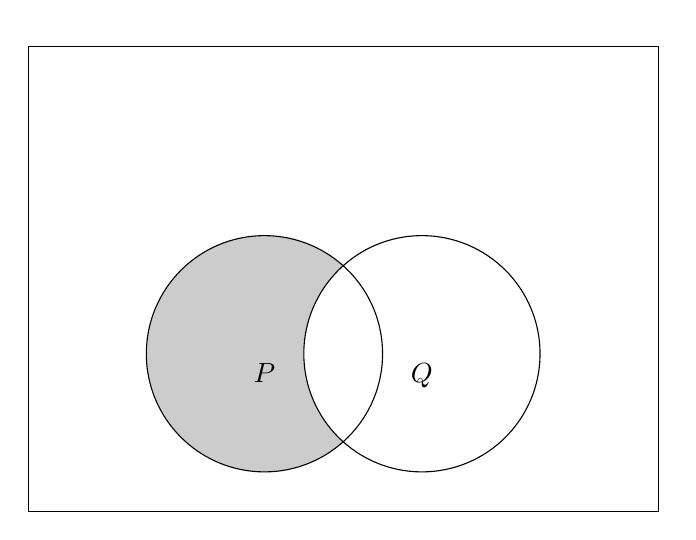
\begin{tikzpicture}
        \begin{scope}[even odd rule]% first circle without the second
        \clip \thirdcircle (-3,-2) rectangle (5,2);
        \fill[gray!40] \firstcircle;
        \end{scope}
        \draw \rectangle node[text=black,above] {};
        \draw \firstcircle node[text=black,below] {$P$};
        \draw \thirdcircle node [text=black,below] {$Q$};
\end{tikzpicture}
\\
$(P^C\uni Q)^C$
\end{figure}
%%%%%%%%%%%%%%%%%%%%%%%%%%%%%%%%%%%%%%%%%%%%%%%%%%%%%%%%%%%%%%%%%%%%%%%%%%%%%%%%%%%%

Entretanto,
\[
[\forall x\in D, p(x)]\to[\forall x\in D, q(x)]
\]
ser\'a verdade quando $P=Q=D$ ou quando $P\neq D$ ($Q$ pode ser qualquer coisa neste caso). $P\subseteq Q$ implica esta condi\caoi, logo a primeira proposi\cao \'e mais forte que a segunda (como observado na se\cao \ref{mquantificadores}).

\paragraph{Excerc\ih cios \ref{conjuntosverdade}}

\begin{enumerate}[{\bf 1.}]
%excercicio1
\item Sejam $D=\{1,2,3,4,5,6,7,8\}$, $p(x)$ ``x \'e par'', $q(x)$, ``$x$ \'e \ih mpar'' e $r(x)$ ``$x$ \'e um n\'umero primo.'' Encontre:
\begin{enumerate}[a)]
\item O conjunto verdade para $p(x)\ee q(x)$.
\item O conjunto verdade para $r(x)\to\nao p(x)$.
\item $P^C\uni Q$.
\item A fun\cao proposicional que tem $\{1,2,3,5,7\}$ como seu conjunto verdade.
\item O conjunto verdade de $\exists x \in D \ni r(x)\to p(x)$.
\item O conjunto verdade de $\forall x\in D, p(x)\ou q(x)$.
\item O conjunto verdade de $[\forall x\in D, p(x)]\ou[\forall x\in D, q(x)]$.
\item O conjunto verdade de $[\forall x\in D, q(x)]\to[\forall x\in D, r(x)]$.
\end{enumerate}

%excercicio2
\item Encontre o conjunto verdade para a fun\cao proposicional ``$x^2-x-2\leq 0$.'' Tome $\mathbb{R}$ como dom\ih nio.

%excercicio3
\item Considere os seguintes pares de proposi\cois. Para cada proposi\cao do par determine as condi\coes para $P,Q$ que garantam que ela seja verdade. E mostrar que sempre que a segunda (de cada par) seja verdade, a primeira dever\'a ser verdade. D\^e um exemplo para mostrar que a primeira pode ser verdade e a segunda falsa.
\begin{enumerate}[a)]
\item $[\forall x\in D, p(x)\ou q(x)]; [\forall x\in D, p(x) \ou \forall x \in D, q(x)]$.
\item $[\exists x\in D\ni p(x)\ee \exists x\in D\ni q(x)];[\exists x\in D\ni p(x)\ee q(x)]$.
\item $[\exists x\in D\ni p(x)\to q(x)];[\exists x\in D\ni p(x) \to \exists x\in D\ni q(x)]$.
\end{enumerate}

%excercicio4
\item {\bf Acredite se quiser:}  

\noindent \textit{\textbf{Conjectura:}} Sejam $A,B$ conjuntos com $B\subseteq A$ e $p$ uma fun\cao proposicional. Ent\ao $\forall x\in A, p(x)$ implica $\forall x\in B, p(x)$  

\noindent \textit{\textbf{``Demonstra\caoi'':}} Suponha que $A,B$ sejam conjuntos como acima e que a implica\cao seja falsa. Ent\ao existe um $z\in B$ tal que $p(z)$ seja falsa. Como $B\subseteq A, \espaco z\in A$. Mas isto significa $\forall x \in A, p(x)$ \'e falso, uma contradi\caoi. 

\noindent \textit{\textbf{``Contraexemplo'':}} Sejam $p(x)$ ``$x<2$,'' $A=\{1,2,3\}$ e $B=\varnothing$. Ent\ao $B\subseteq A$, $\forall x \in A, p(x)$ \'e falso e $\forall x \in B, p(x)$ \'e verdadeiro.
\end{enumerate}
%%%%%%%%%%%%%%%%%%%%%%%%%%%%%%%%%%%%%%%%%%%%%%%%%%%%%%%%%%%%%%%%%%%%%%%%%%%%%%%%%%%%%%%%%%%%

\section{Rela\cois}\label{relacoes}


Sabemos que um conjunto \'e determinado por seus elementos, isto \'e, $\{a,b\}=\{b,a\}$ e a ordem na qual os elementos s\ao listados n\ao faz diferen\cc a. \`As vezes, entretanto, gostar\ih amos de distinguir os elementos listados em ordem diferente. Para isso, introduzimos o conceito de um {\it par ordenado}.\index{Par Ordenado} \'E poss\ih vel definir pares ordenados em termos de conjuntos (veja os ecerc\ih cios no final da sse\caoi), mas esta defini\cao n\ao \'e muito \'util, assim iremos considerar par ordenado como um termo indefinido, em vez disso, definimos as principais propriedades que queremos que os pares ordenados tenham. Nossa nota\cao \'e padr\aoi: um par ordernado com primeiro elemento $a$ e segundo elemento $b$ ser\'a denotado por $(a,b)$. A propriedade na qual estamos interessados \'e:
\begin{definb}
Sejam $(a,b)$ e $(c,d)$ pares ordenados. Ent\ao $(a,b)=(c,d)$ se e somente se $a=c$ e $b=d$.
\end{definb}

Vemos que esta propriedade, de fato, distingue a ordem nos pares ordenados, pois $(a,b)\neq(b,a)$ a menos que $a=b$.  Com este coneito em m\~aos podemos definir uma nova opera\cao de conjuntos, o {\it produto cartesiano} (\`as vezes referido como produto cruzado ou simplesmente produto) de dois conjuntos:
\begin{definb}
Sejam $A,B$ conjuntos. O {\it produto cartesiano}\index{Produto Cartesiano} de $A$ com $B$, denotado por $A\times B$ \'e o conjunto de todos os pares ordenados com primeiro elemento em $A$ e segundo elemento em $B$. Em s\ih mbolos,
\[
A\times B = \{(a,b):\espaco a\in A \text{ e } b\in B\}.
\]
\end{definb}
Por exemplo, se $A=\{1,2,3\}$, $B=\{a,b\}$ e $C=\varnothing$ ent\ao
\begin{equation*}
 \begin{aligned}
A\times B=&\espaco \{(1,a),(1,b),(2,a),(2,b),(3,a),(3,b)\},\\
B\times A=&\espaco \{(a,1),(a,2),(a,3),(b,1),(b,2),(b,3)\},\\
A\times C=&\espaco \varnothing,\\
B\times A=&\espaco \varnothing.
 \end{aligned}
\end{equation*}
Podemos ilustrar $A\times B$ com um arranjo retangular:
\begin{table}[h]
\centering
\begin{tabular}{ccccccc}
\multicolumn{1}{c}{       } &  \multicolumn{1}{c|}{\textit{\textbf b}} & $(1,b)$ & \quad& $(2,b)$ &\quad & $(3,b)$  \\
\multicolumn{1}{c}{{\bf B}} &  \multicolumn{1}{c|}{                  } &         & \quad&         &\quad &          \\
\multicolumn{1}{c}{       } &  \multicolumn{1}{c|}{\textit{\textbf a}} & $(1,a)$ & \quad& $(2,a)$ &\quad & $(3,a)$  \\\cline{3-7}
                            &                               & {\bf 1} & \quad& {\bf 2} &\quad & {\bf 3}   \\
                            &                               &         & \quad& {\bf A} &\quad &           \\
\end{tabular}
\end{table}
Note que $A\times B\neq B\times A$ e que $A\times C=B\times C$ n\ao implica que $A=B$.

Muito frequentemente no Portugu\^es comum (que \'e diferente da linguagem que os matem\'aticos ``falam'') se refere a objetos relacionados a outros. Por exemplo, poder\ih amos dizer, ``Ela est\'a relacionada a mim, ela \'e minha tia'' ou ``A notas que obtenho est\ao relacionadas a quantidade de tempo que estudo.'' Em matem\'atica, rela\coes entre objetos s\ao muito importantes, por isoo queremos este conceito mais preciso. A seguinte defini\cao faz isso, embora provavelmente n\ao seja imediatamente \'obvio  que ela personifica nossa ideia de rela\caoi. 
\begin{definb}
Sejam $A,B$ conjuntos. Uma {\it rela\cao de $A$ em $B$}\index{Rela\caoi} \'e um subconjunto de $A\times B$. Se $R$ \'e uma rela\cao de $A$ em $B$ e $(a,b)\in R$ ser\'a denotada por $aRb$. O {\it dom\ih nio}\index{Rela\caoi!Dom\ih nio} de $R$, denotado por $\Dom(R)$, \'e o conjunto de todos os primeiros elementos dos elementos de $R$, em s\ih mbolos
\begin{equation*}
 \begin{aligned}
\Dom(R)=&\espaco \{a: (a,b)\in R\}\\
      =&\espaco \{a: aRb\}.
 \end{aligned}
\end{equation*}  
A {\it imagem}\index{Rela\caoi!Imagem} de $R$, denotado por $\Ima(R)$, \'e o conjunto de todos os segundos elementos dos elementos de $R$, em s\ih mbolos
\begin{equation*}
 \begin{aligned}
\Ima(R)=&\espaco \{b: (a,b)\in R\}\\
     =&\espaco \{b: aRb\}.
 \end{aligned}
\end{equation*}
Note que, $\Dom(R)\subseteq A$ e $\Ima(R)\subseteq B$. Se $A=B$ dizemos que $R$ \'e uma rela\cao em $A$. 
\end{definb}

Como um exemplo de rela\caoi, suponha que $A=\{1,2,3\}$ e $R$ \'e a rela\cao ``menor que'' em $A$, isto \'e, $aRb$ se e somente se $a<b$. Podemos ilustrar isso com um diagrama, com $\circ$ representando elementos de $A\times A$ e \frame{$\circ$} indicando aqueles pares em $R$:

\begin{table}[h]
\centering
\begin{tabular}{ccccccc}
\multicolumn{1}{c}{       } &  \multicolumn{1}{c|}{{\bf 3}} & \frame{$\circ$} & \quad& \frame{$\circ$} &\quad & $\circ$  \\
\multicolumn{1}{c}{{\bf B}} &  \multicolumn{1}{c|}{{\bf 2}} & \frame{$\circ$} & \quad& $\circ$         &\quad & $\circ$  \\
\multicolumn{1}{c}{       } &  \multicolumn{1}{c|}{{\bf 1}} & $\circ$         & \quad& $\circ$         &\quad & $\circ$  \\\cline{3-7}
                            &                               & {\bf 1} & \quad& {\bf 2} &\quad & {\bf 3}   \\
                            &                               &         & \quad& {\bf A} &\quad &           \\
\end{tabular}
\end{table}
Neste exemplo $\Dom(R)=\{1,2\}$ e $\Ima(R)=\{2,3\}$.

\paragraph{{\bf Exemplos}}
\quad\\[0.3cm]
Antes de procedermos adiante, alguns outros exemplos nos ajudar\ao a fixar as novas ideias em nossas mentes.

\begin{enumerate}[{\bf 1.}]

\item As rela\coes de $A$ em $B$ mais triviais s\ao o conjunto vazio e o produto cartesiano $A\times B$. Na primeira, nenhum elemento de $A$ \'e relacionado com elementos de $B$ e, na segunda, todos elementos de $A$ est\ao relacionados com todos os elementos de $B$. 

\item\label{relex1} Sejam $A$ o conjunto de todas as pessoas vivas no mundo e para $x,y\in A$ defina $xRy$ se e somente se $y$ \'e um dos pais de $x$. Ent\ao $R$ \'e uma rela\cao em $A$. Os pares ordenados pertencentes a $R$ s\ao da forma $(x,\textrm{um dos pais de $x$})$. $\Dom(R)=\{x: \textrm{ um dos pais de $x$ est\'a vivo}\}$ e $\Ima(R)=\{x: \textrm{ $x$ \'e um pai com uma crian\cc a viva.}\}$  

\item\label{relex2} Seja $A=\mathbb{R}$ (o conjunto dos n\'umeros reais) e para $x,y\in \mathbb{R}$ defina $xRy$ se e somente se $y=x^2$. Ent\ao $R$ \'e uma rela\cao em $\mathbb{R}$ e os pares ordenados de $R$ s\ao da forma $(x,x^2)$. De fato, os pares ordenados em $R$ s\ao apenas pares ordenados na fun\cao $y=x^2$, a par\'abola. Na verdade, todas as fun\coes de pr\'e-c\'alculo e c\'alculo s\ao rela\coes em $\mathbb{R}$. Neste exemplo, $\Dom(R)=\mathbb{R}$ e $\Ima(R)=\{x: x\leq 0\}$.

\item\label{relex3} Seja $A$ um conjunto qualquer e para $x,y\in A$ defina $xRy$ e e somente se $x=y$. Ent\ao $R$ \'e uma rela\cao em $A$. Os pares ordenados em $R$ s\ao da forma $(x,x)$. Aqui, $\Dom(R)=\Ima(R)=A$.

\item\label{relex4} Seja $A$ um conjunto qualquer. Se $B,C$ s\ao subconjuntos de $A$ dizemos que $BRC$ se e somente $B\subseteq C$. Ent\ao $R$ \'e uma rela\cao em $\mathbb{P}(A)$ e $\Dom(R)=\Ima(R)=\mathbb{P}(A)$. Em particular, se $A=\{1,2\}$ ent\ao
\[
R=\{(\varnothing,\varnothing),(\varnothing,\{1\}),(\varnothing,\{2\}),(\varnothing,A),(\{1\},\{1\}),(\{1\},A),(\{2\},\{2\}),(\{2\},A),(A,A)\}.
\]

\item\label{relex5} Seja $A$ o conjunto das pessoas do Brasil e seja $B$ o conjunto dos inteirosn positivos menores que $10^{10}$. Ent\ao para $x\in A$ e $y\in B$ dizemos que $xRy$ se e somente se $y$ \'e o n\'umero do CPF de $x$. Ent\ao $R$ \'e uma rela\cao de $A$ em $B$. Os pares ordenados de $R$ s\ao da forma (pessoa, CPF da pessoa).  $\Dom(R)=\{x: x \textrm{ tem CPF}\}$ e $\Ima(R)=\{x: x \textrm{ \'e o CPF de algu\'em}\}$. N\ao podemos listar todos os elementos de $R$ aqui, seria insano!

\item\label{relex6} Seja $A=\{1,2,3\}$ e seja $B=\{1,2\}$ Ent\ao $R=\{(3,1),(3,2)\}$, $S=\varnothing$ e $T=A\times B$ s\ao todos rela\coes de $A$ em $B$. $\Dom(R)=\{3\}$ e $\Ima(R)=\{1,2\}$, $\Dom(R)=\Ima(R)=\varnothing$, $\Dom(R)=A$ e $\Ima(R)=B$. Note que, as rela\coes n\ao precisam ``fazer sentido'' ou ter alguma regra especial ou ter algum padr\aoi. A defini\cao permite que qualquer subconjunto de $A\times B$ seja uma rel\cao de $A$ em $B$.

\item\label{relex7} Sejam $A,B$ conjuntos de proposi\coes e para $p\in A$ e $q\in B$ define-se $xRy$ se e somente se $p\to q$ \'e uma tautologia. Ent\ao $R$ \'e uma rela\cao de $A$ em $B$ e um par ordenado $(p,q)\in R$ se e somente se $q$ \'e uma consequ\^encia l\'ogica de $p$. Podemos pensar na $\Ima(R)$ como o conjunto de todas as conclus\oes que podem ser implicadas logicamente de elementos individuais de $A$ 

\item\label{relex8} Seja $A$ o conjunto de todos os tri\^angulos no plano. Se $s,t\in A$, diremos que $sRt$ se e somente se $s$ \'e similar a $t$ (uma nota\cao que j\'a vem do ensino m\'edio \'e $s\sim t$). Ent\ao $R$ \'e uma rela\cao em $A$ com $\Dom(R)=\Ima(R)=A$ (pois cada tri\^angulo \'e similar a si mesmo).

\item\label{relex9} Seja $\mathbb{R}$ o conjunto dos n\'umeros reais e para $x,y\in\mathbb{R}$ define-se $xRy$ se e somente se $x\leq y$ (note que: $x\leq y$ se e somente se $x<y$ ou $x=y$). Ent\ao $R$ \'e uma rela\cao em $\mathbb{R}$ com $\Dom(R)=\Ima(R)=\mathbb{R}$. Alguns elmentos t\ih picos pertencentes a $R$ s\ao $(2,3)$ $(2,2)$ $(3,\pi)$ $(\pi,4)$ $(2,e)$ ou $(e,3)$.
 
\item\label{relex10} Seja $\mathbb{Z}$ o conjunto dos n\'umeros inteiros e para $x,y\in\mathbb{Z}$ definimos $xRy$ se e somente se $x$ divide $y$, denotados por $x|y$ (note que: isto est\'a definido como: $x|y\leftrightarrow\exists z\in \mathbb{Z},\ni y=xz$. Assim, $3|6$, $2|8$, $-3|6$, $3|-9$ e $2|0$, enquanto que $2$ n\ao divide $9$, denotado por $2\not\vert\espaco 9$). Ent\ao $R$ \'e uma rela\cao em $\mathbb{Z}$ com $\Dom(R)=\Ima(R)=\mathbb{Z}$ (todo inteiro divide a si mesmo). Alguns elementos t\ih picos pertencentes a $R$ s\ao $(1,3)$, $(7,21)$, $(1001,1001)$, $(-1,3)$, $(-2,6)$, $(1001,2002)$ e $(3,0)$.

\item\label{relex11} Seja $\mathbb{N}$ o conjunto dos n\'umeros naturais e para $x,y\in\mathbb{N}$, define-se $xRy$ se e somente se $5|(x-y)$. Ent\ao $R$ \'e uma rela\cao em $\mathbb{N}$ com $\Dom(R)=\Ima(R)=\mathbb{N}$. Alguns exemplos t\ih picos pertencentes a $R$ s\ao $(10,5)$, $(5,10)$, $(3,43)$ e $(482,257)$. 
\end{enumerate}

Observe que nossa maneira de escrever rela\cois, $xRy$, que pode ter parecido um pouco estranho em um primeiro momento, \'e de fato a forma que usualmente escrevemos algumas ``rela\coes bem conhecidas'', como $=$ (igual a), $\leq$ (menor ou igual a), $subseteq$ (subconjunto de), $\sim$ (similar a), $|$ (divide), $\Leftrightarrow$ (logicamente equivalente a). Devemos tamb\'em notar que, muitos dos exemplo acima s\ao familiares a n\'os, s\'o n\ao sab\ih amos que eles eram chamados de rela\cois!

Existem certas propriedades que uma rela\cao me uma conjunto pode ou n\ao ter. Algumas das mais importantes s\ao definidas abaixo:
\begin{definb}\label{reldef1}
Seja $R$ uma rela\cao em um conjunto $A$. Ent\ao dizemos que:
\begin{enumerate}[{\bf a)}]
\item $R$ \'e {\it reflexiva}\index{Rela\caoi!Reflexiva} se e somente se $\forall a\in A,\espaco aRa$.
\item $R$ \'e {\it sim\'etrica}\index{Rela\caoi!Sim\'etrica} se e somente se $\forall a,b\in A,\espaco aRb\to bRa$.
\item $R$ \'e {\it transitiva}\index{Rela\caoi!Transitiva} se e somente se $\forall a,b,c\in A, (aRb\ee bRc)\to aRc$.
\item $R$ \'e {\it antisim\'etrica}\index{Rela\caoi!Antisim\'etrica} se e somente se $\forall a,b\in A, (aRb\ee bRa)\to a=b$.
\item $R$ \'e {\it irrelexiva}\index{Rela\caoi!Irreflexiva} se e somente se $\forall a\in A, \nao(aRa)$.
\item $R$ \'e {\it completa}\index{Rela\caoi!Completa} se e somente se $\forall a,b\in A, a\neq b \to (aRb\ou bRa)$.
\item $R$ \'e {\it assim\'etrica}\index{Rela\caoi!Assim\'etrica} se e somente se $\forall a,b\in A, aRb\to\nao(bRa)$.
\item $R$ \'e uma {\it rela\cao de equival\^encia}\index{Rela\caoi!de Equival\^encia} se e somente se $R$ \'e reflexiva, sim\'etrica e transitiva.
\item $R$ \'e uma {\it ordem parcial}\index{Ordem!Parcial} se e somente se $R$ \'e reflexiva, transitiva e antisim\'etrica. 
\item $R$ \'e uma {\it ordem parcial estrita}\index{Ordem!Parcial Estrita} se e somente se $R$ \'e irreflexiva e transitiva.
\item $R$ \'e uma {\it ordem total (ou ordem linear)}\index{Ordem!Total}\index{Ordem!Linear} se e somente se $R$ \'e uma ordem parcial completa.
\item $R$ \'e uma {\it ordem total estrita }\index{Ordem!Total Estrita} se e somente se $R$ \'e uma ordem parcial estrita completa.
\end{enumerate}
\end{definb}

Pode ser \'util  tentar caracterizar algumas destas propriedades de uma maneira informal para que elas n\ao parecessem t\ao estranhas. Se $R$ \'e reflexiva tudo em $A$ est\'a relacionado a si mesmo. Se $R$ \'e sim\'etrica, ent\ao sempre que $a$ estiver relacionada a $b$ devemos ter $b$ relacionada a $a$. Um exemplo comum de uma rela\cao transitiva \'e a ``prefer\^encia,'' isto \'e, se eu prefiro torta de ma\cc a ao bolo de chocolate e eu prefiro o bolo de chocolate \`a alface murcha, en\tao eu prefiro torta de ma\cc a \`a alface murcha. Se $R$ \'e uma rela\cao antissim\'etrica ent\ao a unica forma de termos ambos $aRb$ e $bRa$ \'e tendo $a=b$. um exemplo para este tipo de rela\cao \'e $\subseteq$, de fato, esta \'e a propriedade que usamos para demonstrar a igualdade de conjuntos. $R$ \'e irreflexiva se nenhum elemento de $A$ est\'a relacionado a si mesmo. A rela\cao ``ser pai de'' \'e irreflexiva. $R$ \'e completa se dados dois elementos distintos em $A$ o primeiro deve estar relacionado com o primeiro ou vice-versa. Um exemplo de uma rela\cao que n\ao \'e comleta \'e $\subseteq$ no conjunto pot\^encia de um conjunto com pelo menos dois elementos (tente encontrar dois subconjuntos que n\ao est\ao relacionados). Normalmente pensamos na prefer\^encia como sendo uma rela\cao assim\'etrica, se eu prefiro torta de ma\cc a ao bolo de chocolate ent\ao eu tamb\'em n\ao prefiro bolo de chocolate \`a torta de ma\cc a. Note que as rela\coes sim\'etricas e antissim\'etricas n\ao s\ao mutualmente exclusivas, uma rela\cao pode ter ambas as propriedades (ou nenhuma delas).

Este pode ser um bom momento para para fazer algums coment\'arios gerais sobre defini\coes matem\'aticas. \'E muito frequente o caso (como nos exemplos acima) que defini\coes d\ao nomes  a objetos que possuem uma certa propriedade. Isto significa que se um certo objeto tem tem a propriedade definida de ``qualquer coisa,'' ent\ao chamaremos isto de ``qualquer coisa,'' e se chamamos um objeto uma ``qualquer coisa'' ent\ao este tem a proriedade definida de ``qualquer coisa.'' Por isso usamos ``se e somente se.'' Se olharmos em muitos livros de matem\'atica (e possivelmente neste livro tamb\'em, por isso fique de olho) encontraremos definic\oes dadas usando apenas ``se-ent\aoi,'' ao inve\'es de ``se e somente se''. Esta \'e conven\cao e escritas matem\'aticas e deve ser entendida como ``se e somente se,'' mesmo quando o ``somente se'' n\ao aparecer explicitamente.

Existe outra caract\ih stica das defini\coes matem\'aticas que muitos estudantes podem achar deconcertantes. Quando vamos a um dicion\'ario para ver a defini\cao de uma nova palavra, esperamos sair com alguma ideia de que a palaravra significa. Por outro lado, uma defini\cao matem\'atica muito raramente d\'a muita ajuda de forma a entend\^e-la, usualmente ela diz de forma oculta a defini\cao das propriedades e as consequ\^encias destas propriedades (e portanto o ``significado'') s\ao desenvolvidas por teoremas e exemplos que seguem. Se pensarmos na defini\cao de derivada em c\'aculo, n\ao h\'a muito significado naquele limite, de fato o maior esfor\cc o em um primeiro curso de c\'aculo \'e direcionado a dar significado a esta defini\caoi. As defini\coes matem\'aticas s\ao importantes, mesmo se elas n\ao contribuem imediatamente ao nosso entendimento? A reposta \'e sim, elas s\ao muito importantes. Sem defini\coes precisas n\ao podemos executar qualquer demonstra\caoi, assim, n\ao devemos esperar sermos capazes de demonstrar que uma dada rela\cao \'e reflexiva sem sabermos a defini\cao de {\it reflexiva}. Devemos esperar obter muitos significados de uma defini\cao matem\'atica? A resposta \'e n\aoi, este n\ao \'e o prop\'osito de uma defini\cao matem\'atica. O significado de termos matem\'aticos \'e desenvolvido atrav\'es de teoremas e exemplos.  

Quando confrontado a uma nova defini\cao de um novo conceito, uma atividade \'util \'e tentar contruir exemplos de objetos apropriados que satisf\cc am a defini\cao e exemplos que n\ao satisfa\cc am. Isto ajuda a tornar algumas das consequ\^encias da defini\cao mais aparentes e ajuda a tornar os conceitos mais concretos. Para ajudar a estabelecer este bom h\'abito vamos come\cc ar olhando para alguns exemplos relacionados as adefini\coes acima (o leitor deve verificar que afirma\coes feitas e criar por si pr\'oprio alguns outros exemplos): com $A=\{1,2,3,4\}$, seja
\begin{equation*}
 \begin{aligned}
R=&\espaco\{(1,2),(2,3)\},\\
S=&\espaco\{(1,1),(2,2),(1,2),(2,1),(3,4)\},\\
T=&\espaco\{(1,1),(2,2),(3,3),(4,4)\}.
 \end{aligned}
\end{equation*} 
Ent\aoi, $R$ \'e n\ao reflexiva, n\ao sim\'etrica, antissim\'etrica, irreflexiva, n\ao completa e assim\'etrica. $S$ \'e n\ao reflexiva, n\ao sim\'etrica, transitiva, n\ao antissim\'etrica, n\ao irreflexiva, n\ao completa e n\ao assim\'etrica. $T$ \'e reflexiva, sim\'etrica, transitiva, antissim\'etrica, n\ao irreflexiva, n\ao completa e n\ao assim\'etrica.

Seria \'util ter algumas figuras destas propriedades. Com $A=\{1,2,3,4\}$, ent\ao se $R$ \'e reflexiva, a mesma deve conter pelo menos a diagonal principal (os quadrados na figura abaixo):

\begin{table}[h]
\centering
\begin{tabular}{ccccccccc}
\multicolumn{1}{c}{       } &  \multicolumn{1}{c|}{{\bf 4}} & $\circ$ & \qquad& $\circ$ &\quad & $\circ$ &\qquad & \frame{$\circ$} \\
\multicolumn{1}{c}{       } &  \multicolumn{1}{c|}{       } &         & \qquad&         &\quad &         &      &         \\
\multicolumn{1}{c}{       } &  \multicolumn{1}{c|}{{\bf 3}} & $\circ$ & \qquad& $\circ$ &\quad & \frame{$\circ$} &\qquad & $\circ$ \\
\multicolumn{1}{c}{{\bf A}} &  \multicolumn{1}{c|}{       } &         & \qquad&         &\quad &         &      &         \\
\multicolumn{1}{c}{       } &  \multicolumn{1}{c|}{{\bf 2}} & $\circ$ & \qquad& \frame{$\circ$} &\quad & $\circ$ &\qquad & $\circ$ \\
\multicolumn{1}{c}{       } &  \multicolumn{1}{c|}{       } &         & \qquad&         &\quad &         &      &         \\
\multicolumn{1}{c}{       } &  \multicolumn{1}{c|}{{\bf 1}} & \frame{$\circ$} & \qquad& $\circ$ &\quad & $\circ$ &\qquad & $\circ$ \\\cline{3-9}
                            &                               & {\bf 1} & \qquad& {\bf 2} &\quad & {\bf 3} &\qquad & {\bf 4} \\
                            &                               &         &      &         &{\bf A}&        &      &         \\
\end{tabular}
\end{table}

Se $R$ \'e sim\'etrica, ent\ao seu gr\'afico deve ser sim\'etrico com respeito a diagonal principal, isto \'e, se $(2,3)$ e $(4,2)$ s\ao elementos de $R$ ent\ao $(3,2)$ e $(2,4)$ devem pertencer a $R$ tamb\'em:

\begin{table}[h]
\centering
\begin{tabular}{ccccccccc}
\multicolumn{1}{c}{       } &  \multicolumn{1}{c|}{{\bf 4}} & $\circ$ & \qquad& \frame{$\circ$} &\quad & $\circ$ &\qquad & $\circ$ \\
\multicolumn{1}{c}{       } &  \multicolumn{1}{c|}{       } &         & \qquad&         &\quad &         &       &         \\
\multicolumn{1}{c}{       } &  \multicolumn{1}{c|}{{\bf 3}} & $\circ$ & \qquad& \frame{$\circ$} &\quad & $\circ$ &\qquad & $\circ$ \\
\multicolumn{1}{c}{{\bf A}} &  \multicolumn{1}{c|}{       } &         & \qquad&         &\quad &         &       &         \\
\multicolumn{1}{c}{       } &  \multicolumn{1}{c|}{{\bf 2}} & $\circ$ & \qquad& $\circ$ &\quad & \frame{$\circ$} &\qquad & \frame{$\circ$} \\
\multicolumn{1}{c}{       } &  \multicolumn{1}{c|}{       } &         & \qquad&         &\quad &         &       &         \\
\multicolumn{1}{c}{       } &  \multicolumn{1}{c|}{{\bf 1}} & $\circ$ & \qquad& $\circ$ &\quad & $\circ$ &\qquad & $\circ$ \\\cline{3-9}
                            &                               & {\bf 1} & \qquad& {\bf 2} &\quad & {\bf 3} &\qquad & {\bf 4} \\
                            &                               &         &      &         &{\bf A}&        &      &         \\
\end{tabular}
\end{table}

Vemos que os exemplos dados anteriormente tamb\'em satisfazem algumas destas propriedades. Por exemplo, $=$ e $\sim$ s\ao rela\coes de equival\^encia, $\leq$ e $\subseteq$ s\ao ordens parciais, $<$ e $\subset$ s\ao ordens parciais estritas, $\leq$ \'e uma ordem parcial total e $<$ \'e uma ordem prcial total estrita. De fato, podemos pensar em ``rela\cao de equival\^encia'' como uma abstra\cao da ideia de igualdade e ``ordem parcial'' como uma abstra\cao da ideia de ordenamento que temos nos n\'umeros reais. Isto da um bom exemplo do poder da abstra\caoi. Podemos pensar na rela\coes de equival\^encia como contendo a ``ess\^encia'' das ideias de igualdade (reflexiva, sim\'etrica e transitiva), qualquer coisa que fa\cc amos com isso pode pararecer uma ideia distante, mas n\ao \'e, lembre-se disso. Como podemos imaginar, mais a frente vamos demonstrar alguns fatos interessantes e \'uteis sobre rela\coes de equival\^encia. No meio tempo temos alguns exerc\ih cios para fazer eassim checar nosso entendimento sobre este assunto. Mas primeiro, um exemplo de teorema e demonstra\cao envolvendo algumas dessa ideias e uma discuss\ao das forma de demonstra\caoi.

\begin{teob}
Seja $A$ um conjunto n\ao vazio. Suponha que $R$ \'e uma rela\cao em $\mathbb{P}(A)$ definida por $BRC$ se e somente se $B\subset C$. Ent\ao $R$ \'e transitiva e irreflexiva, isto \'e, $\subset$ \'e uma ordem parcial estrita.
\end{teob}
\begin{proof}
Suponha que $B,C$ e $D$ sejam subconjuntos de $A$ com $B\subset C$ e $C\subset D$. Para mostrar que $\subset$ \'e transitiva devemos mostrar que $B\subset D$.  Seja $a\in B$. Ent\ao como $B\subset C$, $a\in C$.  Tamb\'em, como $C\subset D$, $a\in C\to a\in D$. Quase terminamos, como j\'a temos $B\subseteq D$, o que falta \'e mostrar que $B$ \'e um subconjunto pr\'oprio de $D$, isto \'e, $B\neq D$. Mas, como $B\subset C$, en\tao existe um $x\in C$ tal que $x\notin B$. Portanto, $x$ deve necessariamente ser um elemento de $D$, pois $C\subset D$. Assim $B\neq D$ e $\subset$ \'e transitiva. Para mostrar que $\subset$ \'e irreflexiva, seja $B\in \mathbb{P}(A)$. Ent\ao $B\not\subset B$, pois $B=B$, e portanto temos que $\forall B\in \mathbb{P}(A),\espaco\nao(B\subset B)$.
\end{proof}
\\

Vamos parar um momento para pensar sobre as formas de demonstra\cao para estas propriedades. Iremos considerar alguns tipos representativos, deixando alguns outros como exerc\ih cios. Suponha que $R$ seja uma rela\cao em um conjunto n\ao vazio $A$. Uma prova direta que $R$ \'e reflexivo teria a forma: Seja $a\in A$.
\\
\ldots
\\ 
``alguma coisa ou outra dependendo de $R$''
\\
\ldots
\\
portanto, $(a,a)\in R$ e $R$ \'e reflexiva.

Para demonstrar simetria: Sejam $a,b\in A$ com $(a,b)\in R$.
\\
\ldots
\\ 
``alguma coisa ou outra dependendo de $R$''
\\
\ldots
\\
portanto, $(b,a)\in R$ e $R$ \'e sim\'etrica.

Para transitividade: Sejam $a,b,c\in A$ com $(a,b)\in R$ e $(b,c)\in R$.
\\
\ldots
\\ 
``alguma coisa ou outra dependendo de $R$''
\\
\ldots
\\
portanto, $(a,c)\in R$ e $R$ \'e transitiva.

Para completude: Sejam $a,b\in A$ com $a\neq b$. Suponha que $(a,b)\notin R$.
\\
\ldots
\\ 
``alguma coisa ou outra dependendo de $R$''
\\
\ldots
\\
portanto, $(b,a)\in R$ e $R$ \'e completa.

Note que nesta \'ultima demonstra\cao usamos nossa t\'ecnica usual para a conclus\ao que \'e uma disjun\caoi. Assumimos que subproposi\cao era falsa e ent\ao provamos que a outra deve ser verdade. Vale tamb\'em a pena notar que em cada caso nosso ponto de partida foi determinado pela conclus\ao e n\ao pelas hip\'oteses que teria a ver com quaisquer propriedades que $R$ tivesse.

\paragraph{Excerc\ih cios \ref{relacoes}}

\begin{enumerate}[{\bf 1.}]
%excercicio1
\item Sejam $A=\{a,b,c\}$, $B=\{1,2\}$ e $C=\{4,5,6\}$
\begin{enumerate}[a)]
\item Liste os elementos de $A\times B$, $B\times A$, e $A\times C$.
\item D\^e exemplos de rela\coes de $A$ em $B$ e de $B$ em $A$, cada uma dos quais tem quatro elementos.
\item D\^e exemplo de uma rela\cao sim\'etrica em $C$ que tenha tr\^es elementos.
\end{enumerate}

%excercicio2
\item Suponha $A=\{1,2,3\}$. Para cada uma das rela\coes dadas abaixo, liste os elementos de $R$, encontre $\Dom(R)$ e $\Ima(R)$ de diga quais das propriedades da defini\cao \ref{reldef1} $R$ tem:
\begin{enumerate}[a)]
\item $R$ \'e a rela\cao $<$ em A. 
\item $R$ \'e a rela\cao $\geq$ em A.
\item $R$ \'e a rela\cao $\subset$ em $\mathbb{P}(A)$.
\end{enumerate}

%excercicio3
\item Suponha que $A,B,C,D$ sejam conjuntos. Prove ou d\^e contraexemplos para as seguintes conjecturas:
\begin{enumerate}[a)]
\item $A\times(B\uni C)= (A\times B)\uni(A\times C)$.
\item $A\times(B\inter C)=(A\times B)\inter(A\times C)$.
\item $(A\times B)\inter(A^C\times B)=\varnothing$.
\item $(A\subseteq B\ee C\subseteq D)\to A\times C\subseteq B\times D$.
\item $A\uni(B\times C)=(A\uni B)\times(A\uni C)$.
\item $A\inter(B\times C)=(A\inter B)\times(A\inter C)$.
\item $(A\times B)\inter(C\times D)=(A\inter C)\times(B\inter D)$.
\item $A\times(B-C)=A\times B-A\times C$.
\end{enumerate}

%excercicio4
\item Suponha que $R$ seja uma rela\cao em um conjunto n\ao vazio $A$. D\^e a forma de demonstra\cao direta para:
\begin{enumerate}[a)]
\item $R$ \'e antissim\'etrica.
\item $R$ \'e irreflexiva.
\item $R$ \'e assim\'etrica.
\end{enumerate}

%excercicio5
\item Sejam $A=\{1,2,3,4\}$ e $R$ uma rela\cao em $a$. D\^e um exemplo utilizando a representa\cao gr\'afica do que segue, assim como foi feito anteriormente para $R$ reflexiva e sim\'etrica.
\begin{enumerate}[a)]
\item Transitiva
\item Irreflexiva
\item Assim\'etrica
\item Rela\cao de equival\^encia
\end{enumerate}

%excercicio6
\item Sejam $A,B$ conjuntos com $R,S$ rela\coes de $A$ para $B$. Demonstre:
\begin{enumerate}[a)]
\item $\Dom(R\uni S)=\Dom(R)\uni \Dom(S)$.
\item $\Dom(R\inter S)\subseteq \Dom(R)\inter \Dom(S)$ e d\^e um exemplo para mostrar que a igualdade n\ao \'e v\'alida.
\item $\Ima(R\uni S)=\Ima(R)\uni \Ima(S)$
\item $\Ima(R\inter S)\subseteq \Ima(R)\inter \Ima(S)$ e d\^e um exemplo para mostrar que a igualdade n\ao \'e v\'alida.
\end{enumerate}

%excercicio7
\item Seja $A$ um conjunto n\ao vazio. Mostre que
\begin{enumerate}[a)]
\item Se $R=A\times A$ ent\ao $R$ \'e reflexiva, sim\'etrica, transitiva e completa. O que poderia se dizer se $R$ fosse assim\'etrica ou antissim\'etrica? 
\item Se $R=\varnothing$ ent\ao $R$ \'e sim\'etrica, transitiva, assim\'etrica, antissim\'etrica, irreflexiva mas n\ao reflexiva.
\item Se $R=\{(a,a):a\in A\}$ ent\ao $R$ \'e uma rela\cao de equival\^encia e tamb\'em \' antissim\'etrica mas n\ao assim\'etrica.
\end{enumerate}

%excercicio8
\item Referente aos exemplos dados anteriormente nessa se\caoi, mostre que:
\begin{enumerate}[a)]
\item Exemplo \ref{relex1} \'e assim\'etrico mas n\ao reflexiva. 
\item Exemplos \ref{relex3}, \ref{relex11} s\ao rela\coes de equival\^encia.
\item Exemplo \ref{relex3}, \ref{relex4}, \ref{relex9} s\ao ordens parciais.
\item Exemplo \ref{relex2}, \ref{relex10} n\ao s\ao completas.
\item Exemplo \ref{relex9} \'e uma ordem total.
\end{enumerate}

%excercicio9
\item Seja $R$ a rela\cao de equival\^encia dada no exemplo \ref{relex11} acima. Determine todos os elementos nestes conjuntos:
\begin{enumerate}[a)]
\item $\{x:xR1\}$.
\item $\{x:xR2\}$.
\item $\{x:xR7\}$.
\end{enumerate}

%excercicio10
\item Seja $R$ a rela\cao $|$ em $\mathbb{Z}$ descrita no exemplo \ref{relex10} acima.
\begin{enumerate}[a)]
\item Liste tr\^es elementos de $\mathbb{Z}\times\mathbb{Z}$ que n\ao sejam elementos de $R$.
\item Quais dos elementos $(0,0),(0,1),(1,0)$ s\ao elementos de $R$?
\item Prove o seguinte:
\begin{enumerate}[i)]
\item $\forall n\in \mathbb{Z}, n|0$.
\item $\forall n\in \mathbb{Z}, 0|n\to n=0$.
\item $\forall a,b,c\in \mathbb{Z}, (a|b\ee a|c)\to a|(b+c)$.
\item $\forall a,b,c\in \mathbb{Z}, a|b\to a|bc$.
\end{enumerate}
\end{enumerate}

%excercicio11
\item Sejam $R,S$ rela\coes em um conjunto n\ao vazio $A$. Demonstre ou d\^e contraexemplos para as seguintes conjecturas:
\begin{enumerate}[a)]
\item $R$ \'e completa $\to$ $R$ \'e reflexiva.
\item $R$ \'e transitiva e irreflexiva $\to$ $R$ \'e assim\'etrica.
\item $R$ \'e reflexiva $\to$ $R$ n\ao \'e assim\'etrica. 
\item $R$ \'e assim\'etrica $\to$ $R$ n\ao \'e reflexiva.
\item $\Dom(R)\inter \Ima(R)=\varnothing\to$ $R$ \'e transitiva, antissim\'etrica, irreflexiva e assim\'etrica.
\item $R$ uma rela\cao de ordem parcial estrita $\to$ $R$ \'e antissim\'etrica e assim\'etrica. 
\item $R$ n\ao reflexiva $\to$ $R$ \'e irreflexiva.
\item $R$ e $S$ sim\'etrica $\to$ $R\inter S$ sim\'etrica. 
\item $R$ ou $S$ sim\'etrica $\to$ $R\inter S$ sim\'etrica.
\item $R$ e $S$ sim\'etrica $\to$ $R\uni S$ sim\'etrica.
\item $R$ ou $S$ reflexiva $\to$ $R\uni S$ reflexiva.
\item $R$ e $S$ transitiva $\to$ $R\uni S$ transitiva.
\item $R$ e $S$ transitiva $\to$ $R\inter S$ transitiva.
\end{enumerate}

%excercicio12
\item D\^e exemplos (se poss\ih vel) de rela\coes que sejam:
\begin{enumerate}[a)]
\item Reflexiva e sim\'etrica mas n\ao transitiva.
\item Sim\'etrica e transitiva mas n\ao reflexiva.
\item Assim\'etrica mas n\ao antissim\'etrica.
\item Sim\'etrica e antissim\'etrica.
\item Nem reflexiva, nem irreflexiva.
\end{enumerate}

%excercicio13
\item\label{relexer13} Se $R$ \'e uma rela\cao de $A$ para $B$ e $C\subseteq A$, definimos {\it restri\cao de $R$ em $C$},\index{Rela\caoi!Restri\caoi} denotada por $R|_C$, como
\[
\{(x,y)\in R: x\in C\}.
\]
\begin{enumerate}[a)]
\item Sejam $A=B=\{1,2,3,4\}$ e $C=\{2,4\}$. Seja $R$ a rela\cao $<$ de $A$ em $B$. Encontre $R$ e $R|_C$. 
\item Se $R$ \'e uma rela\cao de $A$ em $B$ e $C\subseteq A$, mostre que $\Dom(R|_C)=\Dom(R)\inter C$.
\item Se $R$ \'e uma rela\cao de $A$ em $B$ e $B\subseteq A$, $R|_B$ \'e uma rela\cao em $B$? Prove ou de um contraexemplo. 
\end{enumerate}

%excercicio14
\item (Continua\cao do exerc\ih cio \ref{relexer13}) Suponha que $R$ seja uma rela\cao em $A$ com as propriedades listadas abaixo. Se $B\subseteq A$ e $R|_B$ \'e considerada como uma rela\cao em $A$, quais destas propriedades $R|_B$ deve tamb\'em ter? Prove ou d\^e contraexemplos.
\begin{enumerate}[a)]
\item Sim\'etrica 
\item Transitiva
\item Antisim\'etrica
\end{enumerate}

%excercicio15
\item Suponha que tiv\'essemos definido o par ordenado $(a,b)$ pot
\[
(a,b)=\{\{a\},\{a,b\}\}.
\]
Mostre que com essa defini\cao temos
\[
(a,b)=(c,d)\leftrightarrow(a=c\ee b=d).
\]


%excercicio16
\item Suponha que tiv\'essemos definido ``tripla ordenada'' usando pares ordenados como
\[
(a,b,c)=((a,b),c).
\]
Mostre que a mesma tem a propriedade de ordena\cao desejada, isto \'e:
\[
(a,b,c)=(d,e,f)\textrm{ se e somente se }a=d,b=e,c=f.
\]


%excercicio17
\item Seja $R$ uma ordem total estrita em um conjunto n\ao vazio $A$. Mostre que $R$ tem a propriedade da ``tricotomia,'' isto \'e,
\[
\forall a,b\in A, \textrm{ exatamente um dos seguintes \'e verdade } a=b, aRb, bRa.
\]


%excercicio18
\item\label{relexer17} Seja $R$ uma rela\cao em um conjunto n\ao vazio $A$. O {\it fecho transitivo}\index{Rela\caoi!Fecho Transitivo} de $R$ \'e a menor rela\cao transitiva contendo $R$, isto \'e, se $S$ \'e o fecho transitivo de $R$, e $T$ \'e uma rela\cao qualquer contendo $R$, ent\ao
\[
R\subseteq S\subseteq T.
\]
Criamos defini\coes similares para os fechos reflexivos e sim\'etricos. Vamos denotar estes fechos por $R_{trans}$, $R_{sim}$ e $R_{ref}$. 
\begin{enumerate}[a)]
\item Se $A$=\{1,2,3,4\} e $R=\{(1,2),(1,4),(2,3)\}$, encontre $R_{trans}$, $R_{sim}$ e $R_{ref}$. 
\item Demonstre ou d\^e contraexemplo para as seguintes conjecturas ($R,S$ s\ao rela\coes em um conjunto n\ao vazio $A$):
\begin{enumerate}[i)]
\item $(R\uni S)_{trans}=R_{trans}\uni R_{trans}$.
\item $(R\inter S)_{trans}=R_{trans}\inter R_{trans}$.
\item $(R\uni S)_{sim}=R_{sim}\uni R_{sim}$.
\item $(R\inter S)_{sim}=R_{sim}\inter R_{sim}$.
\item $(R\uni S)_{ref}=R_{ref}\uni R_{ref}$.
\item $(R\inter S)_{ref}=R_{ref}\inter R_{ref}$.
\end{enumerate}
\item O que pode ser dito sobre os correpondentes conceitow de fechos antissim\'etrico e assim\'etrico?
\end{enumerate}

%excercicio19
\item Seja $R$ uma rela\cao em um conjunto n\ao vazio $A$. Suponha que $R$ \'e assim\'etrica e tamb\'em satifaz a condi\cao (\`as vezes tamb\'em chamada de {\it transitividade negativa}\index{Rela\caoi!Transitividade Negativa}):
\[
\forall x,y\in A, xRz\to (xRy\ou yRz).
\]
\begin{enumerate}[a)]
\item Mostre $R$ \'e transitiva. Tais rela\coes s\ao \`as vezes chamadas de {\it ordens fracas}.\index{Ordem!Fraca}
\item Se $R$ fosse transitiva e assim\'etrica, ela tamb\'em deveria satifazer a condi\cao dada acima? Prove ou d\^e um contraexemplo.
\end{enumerate}


%excercicio20
\item Seja $R$ uma rela\cao em um conjunto n\ao vazio $A$. Seja $x\in A$. Definimos uma {\it R-classe}\index{R-classe} de $x$, denotada por $<x>_R$, como
\[
<x>_R:=\{y:yRx\}.
\]
O s\ih mbolo $:=$ significa ``por defini\caoi.''
\begin{enumerate}[a)]
\item Seja $A=\{1,2,3,4\}$ e
\[
R=\{(1,2), (1,3), (2,1), (1,1), (2,3), (4,2)\}.
\] 
Encontre $<1>_R$, $<2>_R$, $<3>_R$ e $<4>_R$. 
\item Mostre que $R$ \'e reflexiva se e somente se $\forall x\in A, x\in <x>_R\espaco$.
\item Mostre que $R$ \'e sim\'etrica se e somente se $\forall x,y\in A, x\in <y>_R\espaco\to\espaco y\in <x>_R$.
\item Mostre que $\forall x\in A, <x>_R\espaco\neq\espaco\varnothing$ se e somente se $\Ima(R)=A$.
\item Suponha que $\Dom(R)=A$ e que $R$ seja sim\'etrica e transitiva. Mostre que
\[
\forall x,y\in A, <x>_R\espaco\subseteq\espaco<y>_R\espaco\to\espaco xRy.
\]
Mostre tamb\'em que,
\[
<x>_R\espaco\subseteq\espaco<y>_R\espaco\to\espaco <x>_R\espaco=\espaco<y>_R.
\]
\item Suponha que $R$ seja sim\'etrica e transitiva. Mostre que:
\[
\forall x,y\in A, <x>_R\espaco\inter <y>_R\espaco\neq\espaco\varnothing\to\espaco <x>_R\espaco=<x>_R.
\]
\end{enumerate}

%excercicio21
\item {\bf Acredite se quiser:}  

\noindent \textit{\textbf{Conjectura:}} Suponha que $A$ e $B$ sejam conjuntos tais que $A\times B=B\times A$. Ent\ao $A=B$.

\noindent \textit{\textbf{``Demonstra\caoi'':}} Suponha $A\times B=B\times A$. Seja $a\in A$, com $b\in B$ tais que $(a,b)\in A\times B$. Como $A\times B=B\times A$, $(a,b)\in B\times A$. Assim $a\in B$ e portanto $A\subseteq B$. Um argumentos similar mostra que $B\subseteq A$.

\noindent \textit{\textbf{``Contraexemplo'':}} Sejam $A=\{1,2,3\}$ e $B=\varnothing$. En\tao $A\times B=B\times A=\varnothing$, mas $A\neq B$. 

%excercicio22
\item {\bf Acredite se quiser:}  

\noindent \textit{\textbf{Conjectura:}} Suponha que $R$ seja uma rela\cao em um conjunto n\ao vazio $A$. Se $R$ \'e n\ao sim\'etrica ent\ao $R$ \'e assim\'etrica. 

\noindent \textit{\textbf{``Demonstra\caoi'':}} Seja $R$ uma rela\cao em um conjunto n\ao vazio $A$. Suponha $a,b\in A$ com $(a,b)\in R$. Como $R$ n\ao \'e sim\'etrica, $(b,a)\notin R$ logo $R$ \'e assim\'etrica.

\noindent \textit{\textbf{``Contraexemplo'':}} Sejam $A=\{1,2,3\}$ e $R=\{(1,2),(2,1),(1,3)\}$. Ent\ao $R$ n\ao \'e sim\'etrica nem assim\'etrica.

%excercicio23
\item {\bf Acredite se quiser:}  

\noindent \textit{\textbf{Conjectura:}} Suponha que $R$ seja uma rela\cao em um conjunto n\ao vazio $A$. Se $R$ \'e sim\'etrica e transitiva ent\ao $R$ \'e reflexiva. 

\noindent \textit{\textbf{``Demonstra\caoi'':}} Suponha que $R$ seja uma rela\cao sim\'etrica e transitiva em um conjunto n\ao vazio $A$. Sejam $a,b\in A$ com $(a,b)\in R$. Como $R$ \'e sim\'etrica, $(b,a)\in R$. Mas $R$ tamb\'em \'e transitiva, logo temos que $(a,a)\in R$ e consequentemente $R$ \'e reflexiva.

\noindent \textit{\textbf{``Contraexemplo'':}} Sejam $a=\{a,b,c\}$ e $R=\{(a,b), (b,a), (a,c), (b,c), (a,a)\}$. Ent\ao $R$ \'e sim\'etrica e transitiva, mas n\ao \'e reflexiva pois $(b,b)\notin R$.
\end{enumerate}
%%%%%%%%%%%%%%%%%%%%%%%%%%%%%%%%%%%%%%%%%%%%%%%%%%%%%%%%%%%%%%%%%%%%%%%%%%%%%%%%%%%%%%%%%%%%

\section{Mais rela\coes}\label{mrelacoes}

Nunca satisfeitos com o que j\'a temos, continuaremos com a tradi\cao estabelecida para ambas proposi\coes e conjuntos e fazer novas revela\coes do passado. Naturalmente precisamos de algumas defini\cois:
\begin{definb}
Seja $R$ uma rela\cao de $A$ em $B$. $R$ {\it inversa},\index{Rela\caoi!Inversa} denotada por $R^{-1}$, \'e a rela\cao de $B$ em $A$ dada por $xR^{-1}y$ se e somente se $yRx$. Em s\ih mbolos,
\[
R^{-1}=\{(x,y):(y,x)\in R\}.
\]
\end{definb}

Observe que, $\Dom(R^{-1})=\Ima(R))$ e $\Ima(R^{-1})=\Dom(R)$. Isto \'e os dom\ih nios e imagens de $R$ e $R^{-1}$ est\ao relacionados pelo fato que o dom\ih nio de um \'e a imagem do outro e vice-versa.

Por exemplo, se $R$ \'e a rela\cao ``pai/m\~ae'' (exemplo \ref{relex1} da se\cao \ref{relacoes}, $xRy\to y$ \'e o pai/m\~ae de $x$) ent\ao $R^{-1}$ \'e a rela\cao ``filho,'' $xR^{-1}y$ se e somente se $y$ \'e ``filho'' de $x$. En\tao se ($x$, pai/m\~ae de $x$)$\in R$ en\tao (pai/m\~ae de $x$, $x$)$\in R^{-1}$. Como outro exemplo disso, se $R$ \'e uma relacao em $\mathbb{N}$ dada por $xRy$ se e somente se $x<y$ en\tao $xR^{-1}y$ se e somente se $y<x$.  

Embora possamos usar opera\coes de conjuntos para obter novas rela\coes de antigas (pois rela\coes s\ao conjuntos) podemos tamb\'em ter uma opera\cao particular para rela\coes chamadas composi\cois:
\begin{definb}
Seja $R$ uma rela\cao de $A$ em $B$ e seja $S$ uma rela\cao de $B$ em $C$. Ent\ao $R$ {\it composta com}\index{Rela\caoi!Composta} $S$, denotada por $S\circ R$, \'e a rela\cao de $A$ em $C$ dada por 
\[
S\circ R=\{(x,z): \exists y\in B\ni [(x,y)\in R\ee (y,z)\in S]\}.
\]
\end{definb}

A raz\ao para a aparente ordem reversa de $S$ e $R$ na nota\cao acima \'e porque esta \'e a forma que escreveremos fun\coes mais a frente (que vem a ser a forma que escrevemos fun\coes tamb\'em, $f(x)$). Observe tamb\'em que, de fato, $S\bola R$ \'e uma rela\cao de $A$ em $C$ pois se $(x,y)\in R$ ent\ao $x\in A$ se e somente se $(y,z)\in S$ ent\ao $z\in C$, logo $S\bola R\subseteq A\times C$.

Um exemplo de como ``construir'' $S\bola R$ a partir de $S$ e $R$ \'e: Sejam $A=\{1,2,3,4\}$, $B=\{a,b,c\}$ e $C=\{4,5,6\}$ e, $R=\{(1,a),(1,b),(3,a)\}$ e $S=\{(a,5),(b,4),(a,6),(c,6)\}$. Ent\ao podemos pensar: ``Quais das segundas coordenadas dos elementos de $R$ coincidem com as primeiras coordenadas dos elementos de $S$?'' Estes elementos ser\ao combinados para produzir os elementos de $S\bola R$. Assim, $(1,a)\in R$ e $(a,5)\in S$ nos d\'a $(1,5)\in S\bola R$. Continuando, obtemos
\begin{center}
$(1,4)\in S\bola R$, pois $(1,b)\in R$ e $(b,4)\in S$.\\
$(3,5)\in S\bola R$, pois $(3,a)\in R$ e $(a,5)\in S$.\\
$(1,6)\in S\bola R$, pois $(1,a)\in R$ e $(a,6)\in S$.\\
$(3,6)\in S\bola R$, pois $(3,a)\in R$ e $(a,6)\in S$.
\end{center}
Logo, $S\bola R=\{(1,5),(1,4),(3,5),(1,6),(3,6)\}$.

Agora enunciaremos mais uma defini\cao e ent\ao estaremos prontos para ver mais exemplos:
\begin{definb}
Seja $A$ um conjunto. A {\it rela\cao identidade}\index{Rela\caoi!Identidade} em $A$, denotada por $I_A$, \'e dada por
\[
I_A=\{(x,x):x\in A\}.
\]
\end{definb}
Reconhecemos isso com a velha amiga relacional, a ``igualdade'', em um novo casaco de respeitabilidade. Assim $aI_Ab$ se e somente se $a=b$.

Exemplo: Seja $A=\{1,2,3\}$ e seja $R$ a rela\cao em $A$ tal que $R=\{(1,2),(1,3),(2,3)\}$. Ent\aoi:
\begin{enumerate}[{\bf a)}]
\item $R^{-1}=\{(2,1),(3,1),(3,2)\}$.
\item $I_A=\{(1,1),(2,2),(3,3)\}$.
\item $R^{-1}\bola R=\{(1,1),(1,2),(2,2),(2,1)\}$.
\item $R\bola R^{-1}=\{(2,2),(2,3),(3,3),(3,2)\}$.
\item $R\bola R=\{(1,3)\}$.
\item $R^{-1}\bola R^{-1}=\{(3,1)\}$.
\item $R\bola I_A=I_A\bola R=\{(1,2),(1,3),(2,3)\}$.
\item $R^{-1}\bola I_A=I_A\bola R^{-1}\{(2,1),(3,1),(3,2)\}$. 
\end{enumerate}
Algumas observa\coes podem ser feitas sobre este exemplo, $R\bola R^{-1}\neq R^{-1}\bola R$, logo a composi\cao de rela\coes n\ao \'e comutativa. Tamb\'em vemos que $R\bola I_A=I_A\bola R=R$ talvez seja verdade para qualquer rela\cao $R$ em um conjunto $A$.

Outro exemplo: Sejam $A=\{1,2,3\}$, $B=\{4,5,6\}$ e $C=\{2,3,4\}$ com $R=\{(1,4),(1,5),(2,6),(3,4)\}$ uma rela\cao de $A$ em $B$ e $S=\{(4,2),(4,3),(6,2)\}$ uma rela\cao de $B$ em $C$. Seria \'util ilustrar o que foi mencionado nestes exemplo com um diagrama:
\begin{figure}[h]
\begin{center}
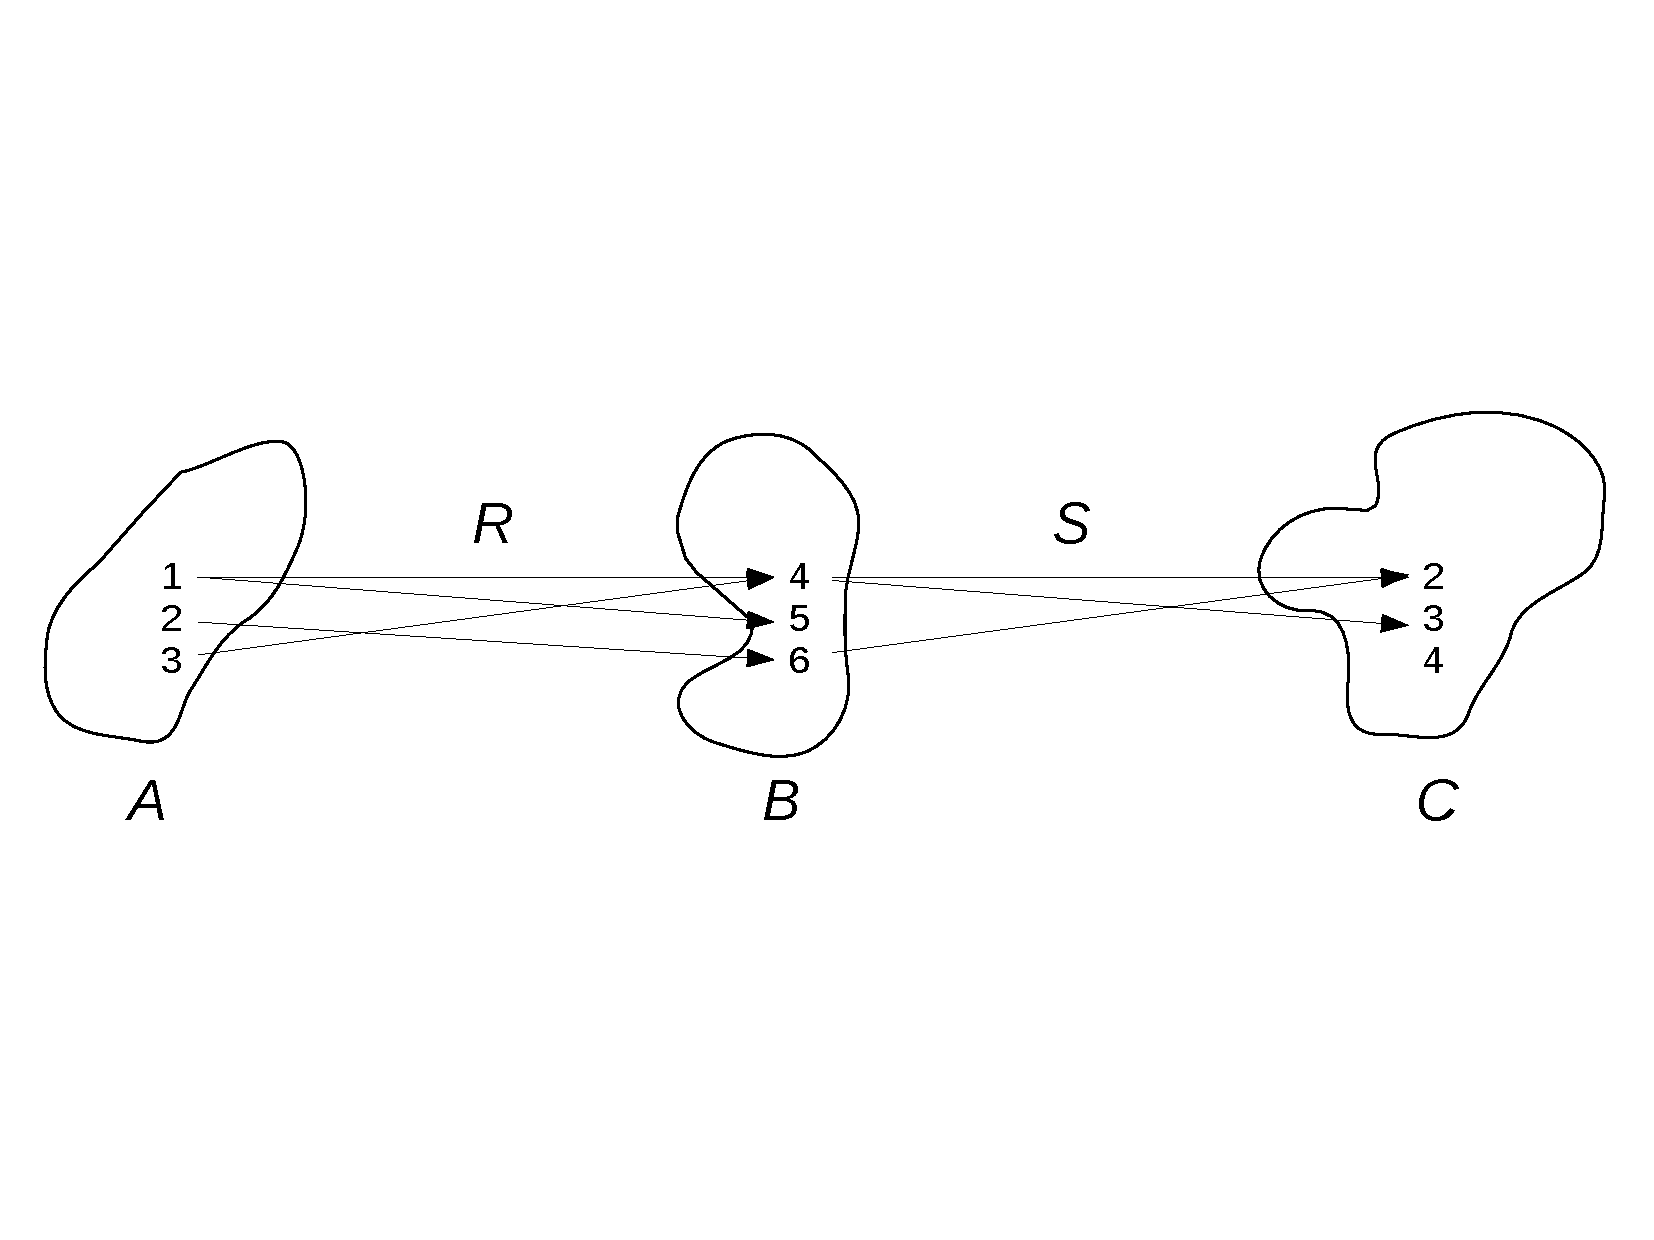
\includegraphics[width=15cm,trim={0.5cm 7cm 0.5cm 6.8cm},clip]{./figuras/figure21.pdf}
\end{center}
\end{figure}

Alguns c\'alculos revelam: 
\begin{enumerate}[{\bf a)}]
\item $S\bola R=\{(1,2),(1,3),(3,2),(3,3),(2,2)\}$.
\item $R^{-1}=\{(4,1),(5,1),(6,2),(4,3)\}$.
\item $S^{-1}=\{(2,4),(3,4),(2,6)\}$.
\item $R^{-1}\bola S^{-1}=\{(2,1),(3,1),(2,3),(2,2),(3,3)\}$.
\item $(S\bola R)^{-1}=\{(2,1),(3,1),(2,3),(3,3),(2,2)\}$.
\end{enumerate}
Note que, $R\bola S$ e $S^{-1}\bola R^{-1}$ n\ao est\ao definidos e que $R^{-1}\bola S^{-1}=(S\bola R)^{-1}$.

Para um pouco mais de pr\'atrica em demonstra\cao de teoremas vamos mostrar que esta ultima igualdade sempre vale:
\begin{teob}
Sejam $A,B,C$ conjuntos, $R$ uma rela\cao de $A$ em $B$ e $S$ uma rela\cao de $B$ em $C$. Ent\ao $(S\bola R)^{-1}=R^{-1}\bola S^{-1}$.
\end{teob}
\begin{proof}
Para esta demonstra\caoi, considere a figura abaixo para manter em mente os v\'arios conjuntos e rela\coes involvidas.
\begin{figure}[h]
\begin{center}
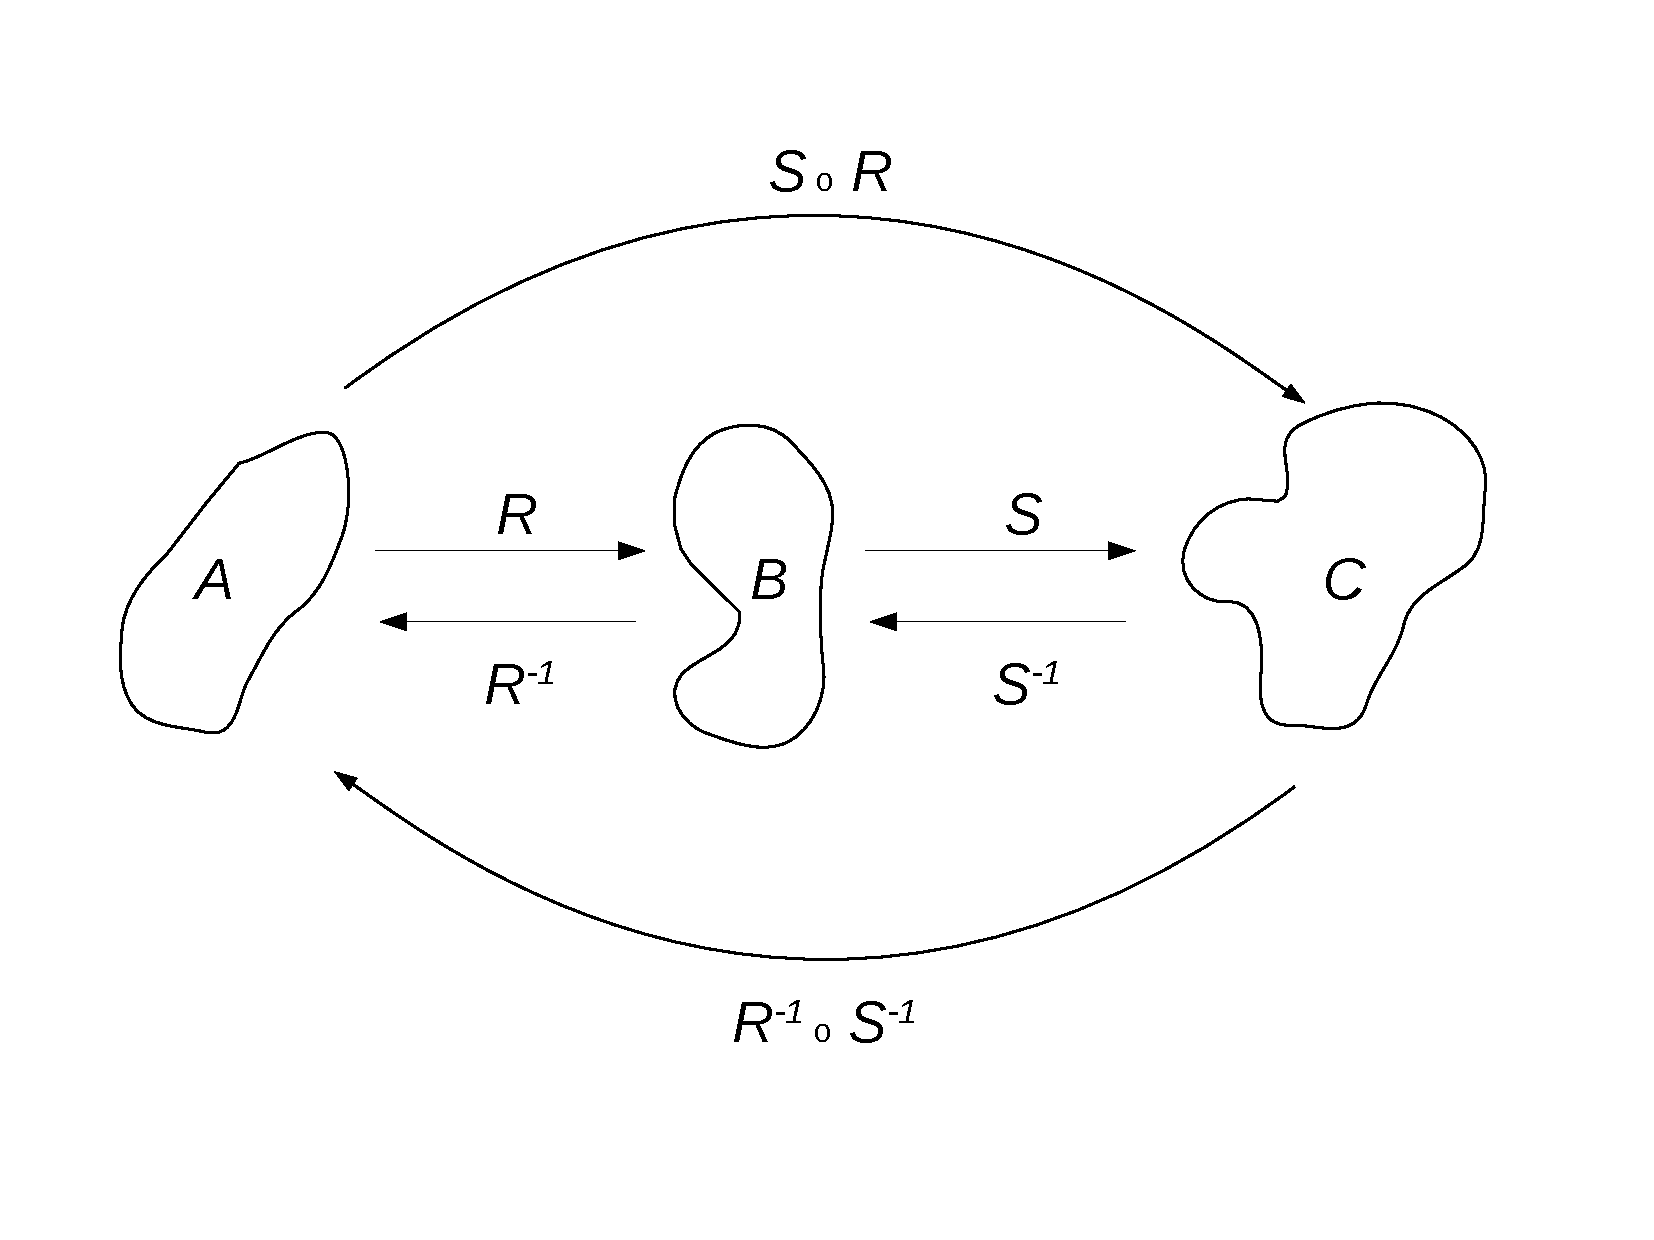
\includegraphics[width=13cm,trim={2cm 2.5cm 2cm 2.5cm},clip]{./figuras/figure22.pdf}
\end{center}
\end{figure}
Primeiro, observe que $(S\bola R)^{-1}$ \'e uma rela\cao de $C$ em $A$ assim como $(S\bola R)^{-1}$, isso diz que estas rela\coes t\^em a chance de serem iguais. Lembrando que rela\coes s\ao conjuntos, portanto para mostrar que duas rela\coes s\ao iguais, devemos mostrar que elas s\ao iguais como conjuntos. Para come\cc ar, seja $(x,z)\in (S\bola R)^{-1}$. Ent\ao $(z,x)\in S\bola R$, logo existe um $y\in B$ tal que $(z,y)\in R$ e $(y,x)\in S$. Consequentemente, $(y,z)\in R^{-1}$ e $(x,y)\in S^{-1}$. Portanto, $(x,z)\in R^{-1}\bola S^{-1}$, assim $(S\bola R)^{-1}\subseteq R^{-1}\bola S^{-1}$.

Agora para mostrar a outra inclus\ao, seja $(x,z)\in R^{-1}\bola S^{-1}$. Ent\ao existem um $y\in B$, tal que $(x,y)\in S^{-1}$ e $(y,z)\in R^{-1}$. Consequentemente, $(y,z)\in S$ e $(z,y)\in R$, portanto temos $(z,x)\in S\bola R$, logo $(x,z)\in (S\bola R)^{-1}$ como desejado.
\end{proof}
\\

Embora a demonstra\cao anterior possa parecer um pouco complicado, mas cada passo apenas envolveu tradu\cao para linguagem de conjuntos uando as defini\cois, por exemplo $(x,y)\in S^{-1}$ significa que $(y,x)\in S$. Em outras palavras, este resultado nos diz que a inversa de uma composi\cao de rela\coes \'e acomposi\cao das inversas na ordem oposta.

Agora apresentamos um exemplo envolvendo composi\caoi. Seja $A=\{1,2,3\}$, $B=\{4,5,6\}$, $C=\{6,7,8\}$ e $D=\{1,4,6\}$ com
\begin{equation*}
 \begin{aligned}
R=&\espaco\{(1,4),(3,5),(3,6)\} \textrm{ uma rela\cao de $A$ em $B$},\\
S=&\espaco\{(4,6),(6,8)\} \textrm{ uma rela\cao de $B$ em $C$},\\
T=&\espaco\{(6,1),(8,6),(6,4)\} \textrm{ uma rela\cao de $C$ em $D$}.
 \end{aligned}
\end{equation*} 
Estas rela\coes est\ao ilustradas na figura abaixo:
\begin{figure}[h]
\begin{center}
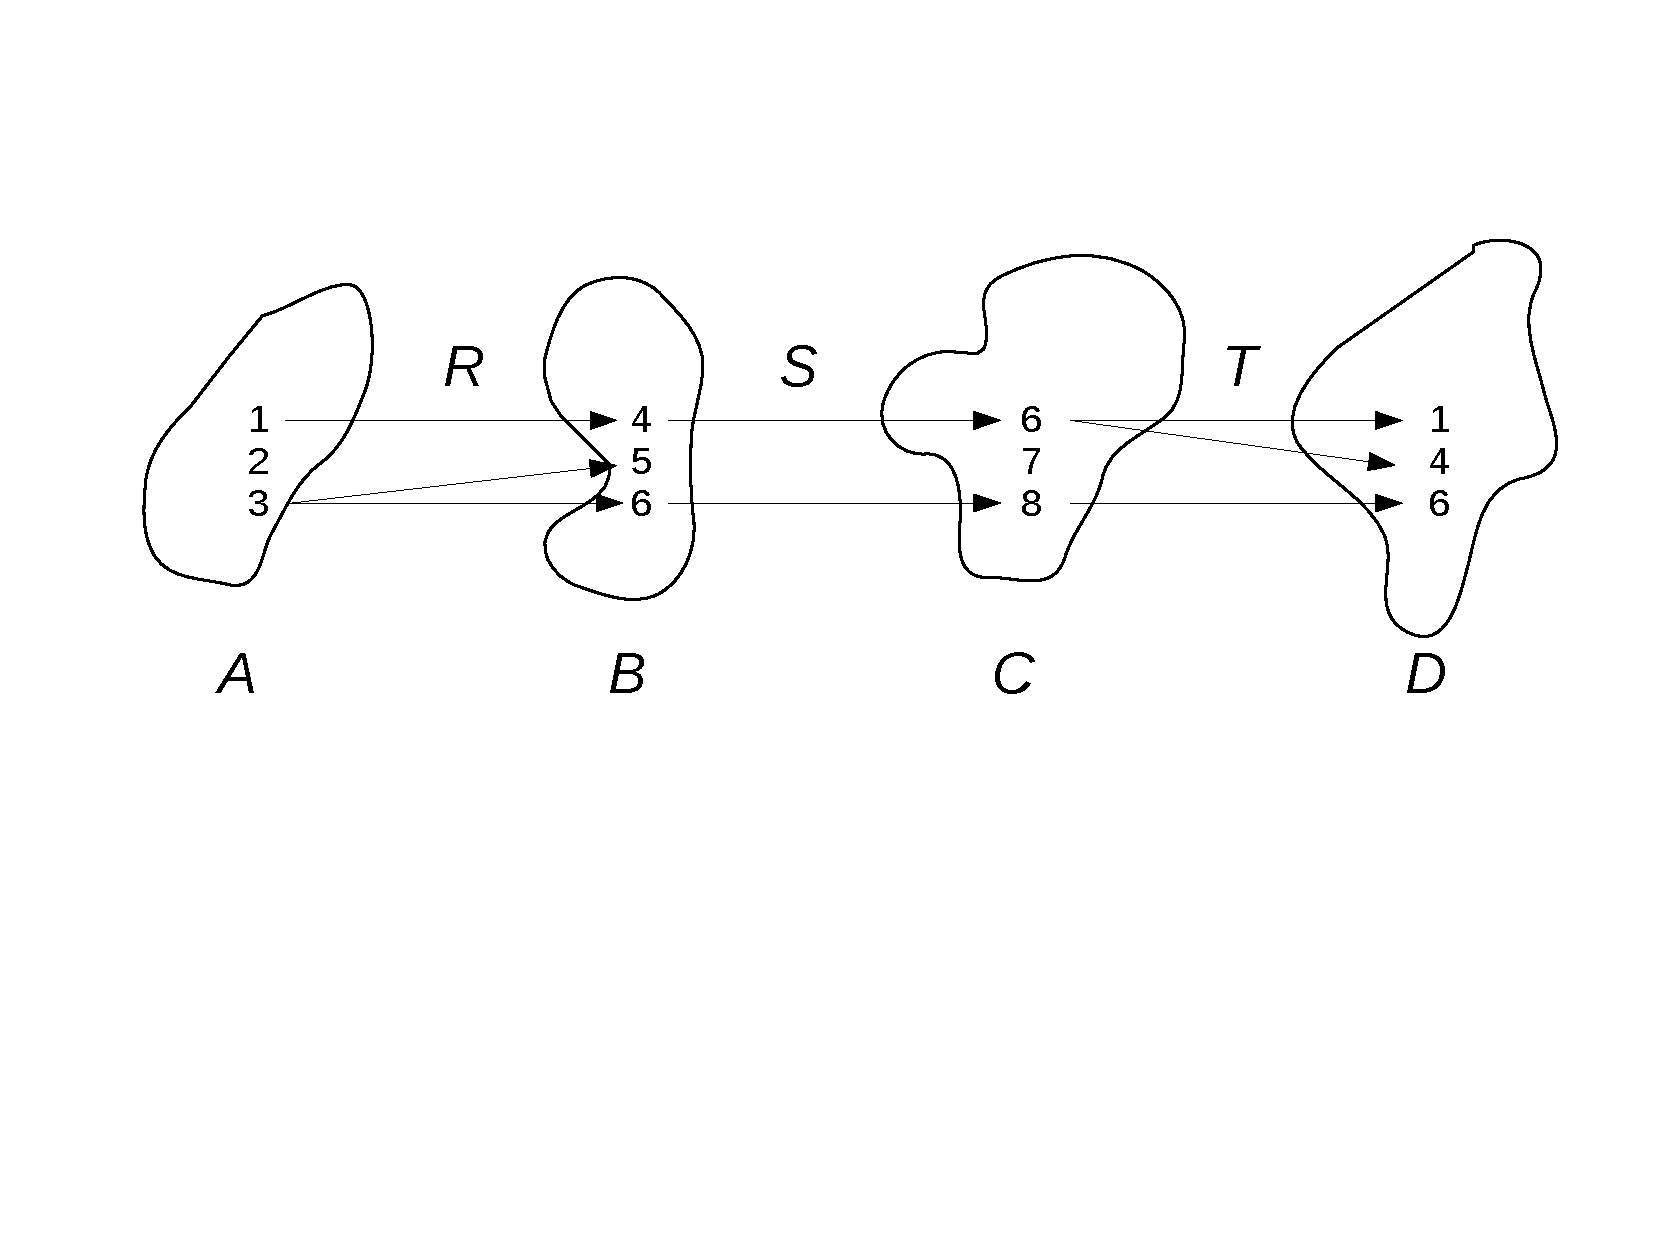
\includegraphics[width=15cm,trim={1.5cm 10cm 1.5cm 4cm},clip]{./figuras/figure23.pdf}
\end{center}
\end{figure}

Ent\ao podemos formar
\begin{equation*}
 \begin{aligned}
S\bola R=&\espaco\{(1,6),(3,8)\} \textrm{ uma rela\cao de $A$ em $C$},\\
T\bola S=&\espaco\{(4,1),(4,4),(6,6)\} \textrm{ uma rela\cao de $B$ em $D$}.
 \end{aligned}
\end{equation*}
Agora, estas podem ser compostas com $T$ e $R$ para obter:
\begin{equation*}
 \begin{aligned}
T\bola(S\bola R)=&\espaco\{(1,1),(1,4),(3,6)\} \textrm{ uma rela\cao de $A$ em $C$},\\
(T\bola S)\bola R=&\espaco\{(1,1),(1,4),(3,6)\} \textrm{ uma rela\cao de $B$ em $D$}.
 \end{aligned}
\end{equation*}

Incrivelmente, estas duas igualdades s\ao iguais! N\ao somos excepcionalmente sortudos em nossas escolhas de $R$, $S$ e $T$. Entretanto, esta igualdade \'e sempre v\'alida. Matem\'aticos expressam isto dizendo ``a composi\cao de rela\coes \'e associativa.''\index{Rela\caoi!Associatividade} Agora apresentamos a demonstra\cao disso:
\begin{teob}\label{relto1}
Sejam $A,B,C$ e $D$ conjuntos com $R$ uma rela\cao de $A$ em $B$, $S$ uma rela\cao de $B$ em $C$ e $T$ uma rela\cao de $C$ em $D$. Ent\ao
\[
T\bola(S\bola R)=(T\bola S)\bola R.
\]
\end{teob}
\begin{proof}
A figura abaixo nos ajudar\'a a ver as v\'arias rela\coes envolvidas:
\begin{figure}[h]
\begin{center}
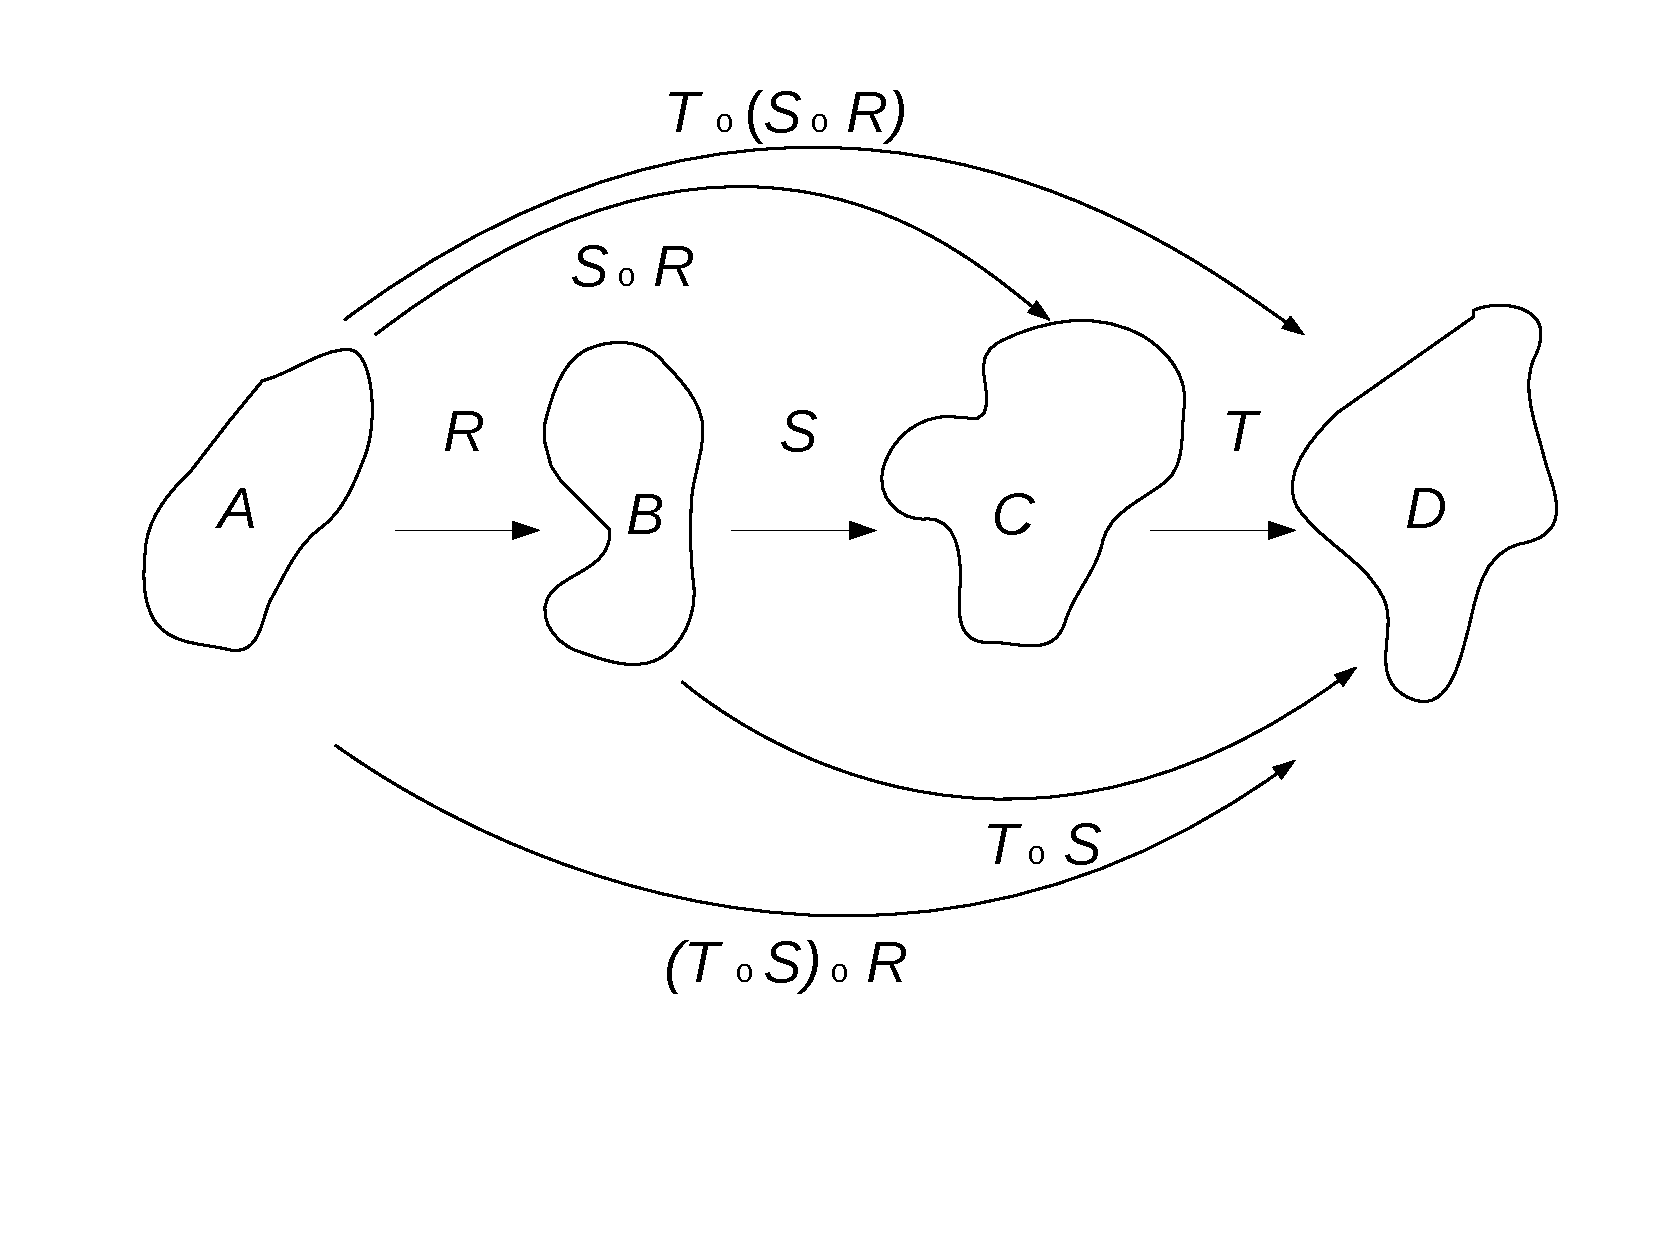
\includegraphics[width=13cm,trim={1cm 1.5cm 1cm 1.5cm},clip]{./figuras/figure24.pdf}
\end{center}
\end{figure}

Precisamos mostras a inclus\ao de conjuntos em ambos os lados. Primeiro, para ver que $T\bola(S\bola R)\subseteq(T\bola S)\bola R$, seja $(x,y)\in T\bola(S\bola R)$. En\tao $x\in A$ e $y\in D$ e exsite $z\in C$ tal que $(x,z)\in S\bola R$ e $(z,y)\in T$. Como, $(x,z)\in S\bola R$, existe $w\in B$ tal que $(x,w) \in R$ e $(w,z)\in S$. Agora, $(w,z)\in S$ e $(z,y)\in T$ implicam que $(w,y)\in T\bola S$. Mas $(x,w) \in R$, assim $(x,y)\in (T\bola S)\bola R$. A demonstra\cao de que a outra inclus\ao \'e v\'alida fica como excerc\ih cio.
\end{proof}
\\

Podemos tambem combinar algumas das propriedades especiais de rela\coes com estas opera\cois. Por exemplo, temos:
\begin{teob}
Seja $R$ uma rela\cao em $A$. Ent\ao $R$ \'e transitiva se e somente se $R\bola R\subseteq R$
\end{teob}
\begin{proof}
Como este teorema \'e uma equival\^encia, temos que demostrar duas implica\cois. Come\cc aremos mostrando que $R$ transitiva implica $R\bola R\subseteq R$. Seja $(x,y)\in R\bola R$. Ent\ao existe $z\in A$ tal que $(x,z)\in R$ e $(z,y)\in R$. Mas, como $R$ \'e transitiva temos que $(x,y)\in R$. Portanto, $R\bola R\subseteq R$.

Agora, mostremos que $R\bola R\subseteq R$ implica que $R$ seja transitiva. Suponha que $(x,y)$ e $(y,z)$ sejam elementos de $R$. Ent\aoi, $(x,z)\in R\bola R$ e como $R\bola R\subseteq R$, $(x,z)$ deve necessariamente ser um elemento de $R$ e assim, $R$ \'e transitiva. 
\end{proof}
\\

N\ao podemos abster-nos de notar mais uma vez qua a forma de demonstra\cao aqui foi determinada pela conclus\ao de cada implica\caoi. Para a primeira, a conclus\ao era $R\bola R\subseteq R$, postanto usamos a t\'ecnica usual de subconjunto para come\cc ar com elemento fixo mas arbitr\'ario em um conjunto e mostrando que este era um elemento do outro conjunto. Na segunda implica\cao, a conclus\ao era que $R$ seria transitiva, neste caso, mostramos que $R$ stisfazia a defini\cao de transitividade. Em ambos os casos as hip\'oteses vieram durante a demonstra\cao e n\ao no come\cc o.

\paragraph{Excerc\ih cios \ref{mrelacoes}}

\begin{enumerate}[{\bf 1.}]

%excercicio1
\item Sejam $A=\{1,2,4\}$ e $B=\{1,3,4\}$. Sejam $R=\{(1,3),(1,4),(4,4)\}$ uma rela\cao de $A$ em $B$, $S=\{(1,1),(3,4),(3,2)\}$ uma rela\cao de $B$ em $A$ e $T=\varnothing$ uma rela\cao de $A$ em $B$. Encontre:
\begin{enumerate}[a)]
\item $\Dom(R)$.
\item $\Dom(S)$.
\item $\Dom(T)$.
\item $\Ima(R)$.
\item $\Ima(S)$.
\item $\Ima(T)$.
\item $S\circ R$.
\item $R\circ S$.
\item $\Dom(S\circ R)$.
\item $\Ima(S\circ R)$.
\item $\Dom(R\circ S)$.
\item $\Ima(R\circ S)$.
\item $R^{-1}$.
\item $S^{-1}$.
\item $I_A$.
\item $I_B$.
\item $R^{-1}\circ S^{-1}$.
\item $S^{-1}\circ R^{-1}$.
\item $(R\circ S)^{-1}$.
\item $(S\circ R)^{-1}$.
\item $T^{-1}$.
\item $I_B^{-1}$.
\item $(R\bola S)\bola R$.
\item $R\bola(S\bola R)$. 
\end{enumerate}

%excercicio2
\item Seja $R$ uma rela\cao em um conjunto n\ao vazio $A$. Mostre que:
\begin{enumerate}[a)]
\item $(R^{-1})^{-1}=R$
\item $I_A^{-1}-I_A$
\item $R$ \'e reflexiva se e somente se $I_A\subseteq R\subseteq R\bola R$.
\item $R$ \'e sim\'etrica se e somente se $R=R^{-1}$.
\item $R$ \'e transitiva se e somente se $R^{-1}$ \'e transitiva.
\item $R$ \'e uma rela\cao de equival\^encia e se somente se $R^{-1}$ \'e uma rela\cao de equival\^encia.
\item Suponha que $\Dom(R)=A$. $R$ \'e uma rela\cao de equival\^encia se e somente se $R=R^{-1}=R\bola R$.
\item $R$ \'a assim\'etrica se e somente se $R\inter R^{-1}=\varnothing$.
\item $R\uni R^{-1}=A\times A$ implica que $R$ \'e completa.
\item $R$ sim\'etrica implica $R\bola R$ \'e sim\'etrica.
\item $I_{\Dom(R)}\subseteq R^{-1}\bola R$.
\item $R$ \'e uma ordem parcial se e somente se $R^{-1}$ \'e uma ordem parcial.
\item $R$ \'e uma ordem parcial se e somente se $R\inter R^{-1}=I_A$ e $R\bola R=R$.
\item $R$ \'e uma ordem parcial estrita se e somente se $R^{-1}$ \'e uma ordem parcial estrita.
\end{enumerate}

%excercicio3
\item Seja $A$ um conjunto n\ao vazio com $R,S$ rela\coes em $A$. Considere as seguintes conjecturas. Prove as verdadeiras e d\^e exemplos para aquelas que s\ao falsas.
\begin{enumerate}[a)]
\item $R$ \'e sim\'etrica implica $R\bola R$ sim\'etrica.
\item $R\bola S^{-1}=S\bola R^{-1}$ implica que $R\bola S^{-1}$ seja sim\'etrica.
\end{enumerate}

%excercicio4
\item Seja $R$ uma rela\cao de $A$ em $B$ e $S$ uma rela\cao  de $B$ em $C$. Mostre que:
\begin{enumerate}[a)]
\item $\Dom(S\bola R)\subseteq \Dom(R)$.
\item $\Ima(S\bola R)\subseteq \Ima(S)$.
\item $\Ima(R)\subseteq \Dom(S)$ implica $\Dom(S\bola R)=\Dom(R)$. A rec\ih proca \'e verdadeira? 
\end{enumerate}

%excercicio5
\item Complete a demonstra\cao do teorema \ref{relto1}.

%excercicio6
\item Suponha que $R$ e $S$ sejam rela\coes de equival\^encia em um conjunto n\ao vazio $A$. Considere as seguintes conjecturas. Prove as verdadeiras e d\^e exemplos para aquelas que s\ao falsas. 
\begin{enumerate}[a)]
\item $R\uni S$ \'e uma rela\cao de equival\^encia implica que $R\bola S=S\bola R$.
\item $R\uni S= R\bola S$ implica que $R\uni S$ \'e uma rela\cao de equival\^encia.
\item $R\uni S= R\bola S$ implica que $R\bola S=S\bola R$.
\end{enumerate}

%excercicio7
\item Seja $R$ a rela\cao $<$ nos inteiros. Mostre que $R$ \'e uma ordem parcial estrita. Tamb\'em mostre que $R\uni I_{\mathbb{Z}}$ (que \'e $\leq$) \'e uma ordem parcial.

%excercicio8
\item Seja $R$ uma ordem parcial em um conjunto n\ao vazio $A$. Mostre que $R-I_A$ \'e uma ordem parcial estrita em $A$.

%excercicio9
\item Seja $R$ uma rela\cao em um conjunto n\ao vazio $A$. Prove ou d\^e contraexemplos (refira-se ao excerc\ih cio \ref{relexer17}, da se\cao \ref{relacoes}):
\begin{enumerate}[a)]
\item $R_{ref}=R\uni I_A$. 
\item $R_{sim}=R\uni R^{-1}$.
\item $R_{trans}=R\uni (R\bola R)$.
\end{enumerate}

%excercicio10
\item Sejam $R,S$ e $T$ rela\coes entre conjuntos. Determine algumas condi\coes sobre $R,S$ e $T$ para garantir as seguintes conclus\ois. Demonstre que suas conjecturas est\ao corretas.
\begin{enumerate}[a)]
\item $R\bola S=R\bola T$ implica $S=T$.
\item $S\bola R=T\bola R$ implica $S=T$.
\end{enumerate}

%excercicio11
\item {\bf Acredite se quiser:}  

\noindent \textit{\textbf{Conjectura:}} Seja $R$ uma rela\cao em um conjunto n\ao vazio $A$. Se $R$ \'e transitiva ent\ao $R\bola R$ \'e transitiva.

\noindent \textit{\textbf{``Demonstra\caoi'':}} Seja $R$ uma rela\cao transitiva em $A$. Sejam $a,b,c\in A$ com $(a,b),(b,c)\in R\bola R$. Ent\ao existem $d,e\in A$ tais que $(a,d),(d,b),(b,e),(e,c)\in R$. Como $R$ \'e transitiva $(a,b),(b,c)\in R$, isso implica que $(a,c)\in R\bola R$, logo $R\bola R$ \'e transitiva.

\noindent \textit{\textbf{``Contraexemplo'':}} Seja, $A=\{1,2,3\}$ $R=\{(1,2),(2,2),(2,3),(1,3)\}$. Assim,
\[
R\bola R=\{(1,3),(1,2),(2,3),(2,2)\},
\]
logo temos $R$ transitiva e $R\bola R$ n\aoi.

%excercicio12
\item {\bf Acredite se quiser:}  

\noindent \textit{\textbf{Conjectura:}} Sejam $R,S$ rela\coes de equival\^encia em um conjunto n\ao vazio $A$. Se $R\bola S=S\bola R$ ent\ao $R\uni S$ \'e uma rela\cao de equival\^encia.

\noindent \textit{\textbf{``Demonstra\caoi'':}} Sejam $R,S$ como acima. Claramente, $R\uni S$ \'e reflefiva. Se $(a,b)\in R\uni S$ ent\ao $(a,b)\in R$ ou $(a,b)\in S$. Se $(a,b)\in R$, e como $R$ \'e sim\'etrica, $(b,a)\in R$, logo $(b,a)\in R\uni S$. Por argumentos semelhantes, se $(a,b)\in S$ ent\ao $(b,a)\in S$, isto demonstra que $R\uni S$ \'e sim\'trica. Aogra, sejam $(a,b),(b,c)\in R\uni S$. Se ambos pertencem a $R$, ou se ambos pertencem a $S$, a transitividade de cada um implica que $R\uni S$ \'e transitiva. Portanto, suponha que $(a,b)\in R$ e $(b,c)\in S$. Como $R\bola S=S\bola R$ e $(a,c)\in S\bola R$, $(a,c)\in R\bola S$. Assim existe $d\in A$ tal que $(a,d)\in S$ e $(d,c)\in R$. Mas, ambos $R$ e $S$ s\ao sim\'etricos, portanto $(c,d)\in R$ e $(d,a)\in S$. Logo, $(c,a)\in R$. Mas $R$ \'e sim\'etrica, assim temos $(a,c)\in R$ e consequentemente $R\uni S$ \'e transitiva. Argumentos similares podem ser utilizados no caso $(a,b)\in S$ e $(b,c)\in R$.

\noindent \textit{\textbf{``Contraexemplo'':}} Sejam 
\begin{equation*}
 \begin{aligned}
A=&\{a,b,c,d\},\\
R=&I_A\uni\{(a,b),(b,a),(a,c),(c,a)\},\\
S=&I_A\uni\{(c,d),(d,c),(a,c),(c,a),(d,a),(a,d)\}.
 \end{aligned}
\end{equation*}
Ent\ao $R,S$ s\ao rela\coes de equival\^encia com $R\bola S=S\bola R$, mas $R\uni S$ cont\'em $(b,a)$ e $(a,d)$ mas n\ao $(b,d)$ e assim n\ao \'e transitiva.

%excercicio13
\item {\bf Acredite se quiser:}  

\noindent \textit{\textbf{Conjectura:}} Seja $R$ uma ordem total estrita em um conjunto n\ao vazio $A$. Ent\ao $S=(A\times A)-R$ \'e uma ordem total em $A$. 

\noindent \textit{\textbf{``Demonstra\caoi'':}} Como $R$ \'e irreflexiva, $I_A\inter R=\varnothing$ portanto $I_A\subseteq S$ e $S$ \'e reflexiva. Agora suponha que $(a,b),(b,c)\in S$. $R$ \'e completa, assim como $(a,b),(b,c)\in S$, temos que $(b,a),(c,b)\in R$. A trnasitividade de $R$ implica que $(c,a)\in R$. Se $(a,c)\in R$ ent\ao $(a,a)\in R$, que \'e imposs\ih vel, consequentemente $(a,c)\in S$ e $S$ \'e transitiva. Agora, suponha que $(a,b),(b,a)\in S$. Ent\ao devemos ter $a=b$, caso contr\'ario $R$ n\ao seria completa. Assim $S$ \'e uma ordem parcial. Se $a,b\in A$, $a\neq b$ e $(a,b)\notin S$, ent\ao $(a,b)\in R$, e como notado anteriormente, isto implica $(b,a)\in S$ e consequentemente $S$ \'e completa e assim uma ordem total.

\noindent \textit{\textbf{``Contraexemplo'':}} Sejam $A=\{1,2,3\}$ e $R=\{(1,2),(2,3),(3,1)\}$. Ent\ao
\[
S=\{(1,1),(2,2),(3,3),(2,1),(1,3),(3,2)\}
\]
n\ao \'e uma ordem total pois n\ao \'e transitiva ($(1,3),(3,2)\in S$, mas $(1,2)\notin S$).
\end{enumerate}
%%%%%%%%%%%%%%%%%%%%%%%%%%%%%%%%%%%%%%%%%%%%%%%%%%%%%%%%%%%%%%%%%%%%%%%%%%%%%%%%%%%%%%%%%%%%

\section{Rela\coes de Equival\^encia e Parti\cois}\label{equivalencia}

Vamos dar uma olhada mais de perto nas rela\coes de equival\^encia $R$ que estavam no exemplo \ref{relex11} da se\cao \ref{relacoes} (lembremos que $R$ era uma rela\cao em $\mathbb{N}$ dada por $xRy$ se e somente se $5|(x-y)$). Se definirmos $S_i=\{x: xRi\}$, vemos que:
\begin{equation*}
 \begin{aligned}
S_1&=\{x: xR1\}=\{1,6,11,16,\ldots\},\\
S_2&=\{x: xR2\}=\{2,7,12,17,\ldots\},\\
S_3&=\{x: xR3\}=\{3,8,13,18,\ldots\},\\
S_4&=\{x: xR4\}=\{4,9,14,19,\ldots\},\\
S_5&=\{x: xR5\}=\{5,10,15,20,\ldots\},\\
S_6&=\{x: xR6\}=\{1,6,11,16,\ldots\}=S_1,\\
S_7&=S_2,\\
S_8&=S_3,\\
& \vdots\\
 \end{aligned}
\end{equation*}
ou melhor graficamente:

\begin{figure}[h]
\begin{center}
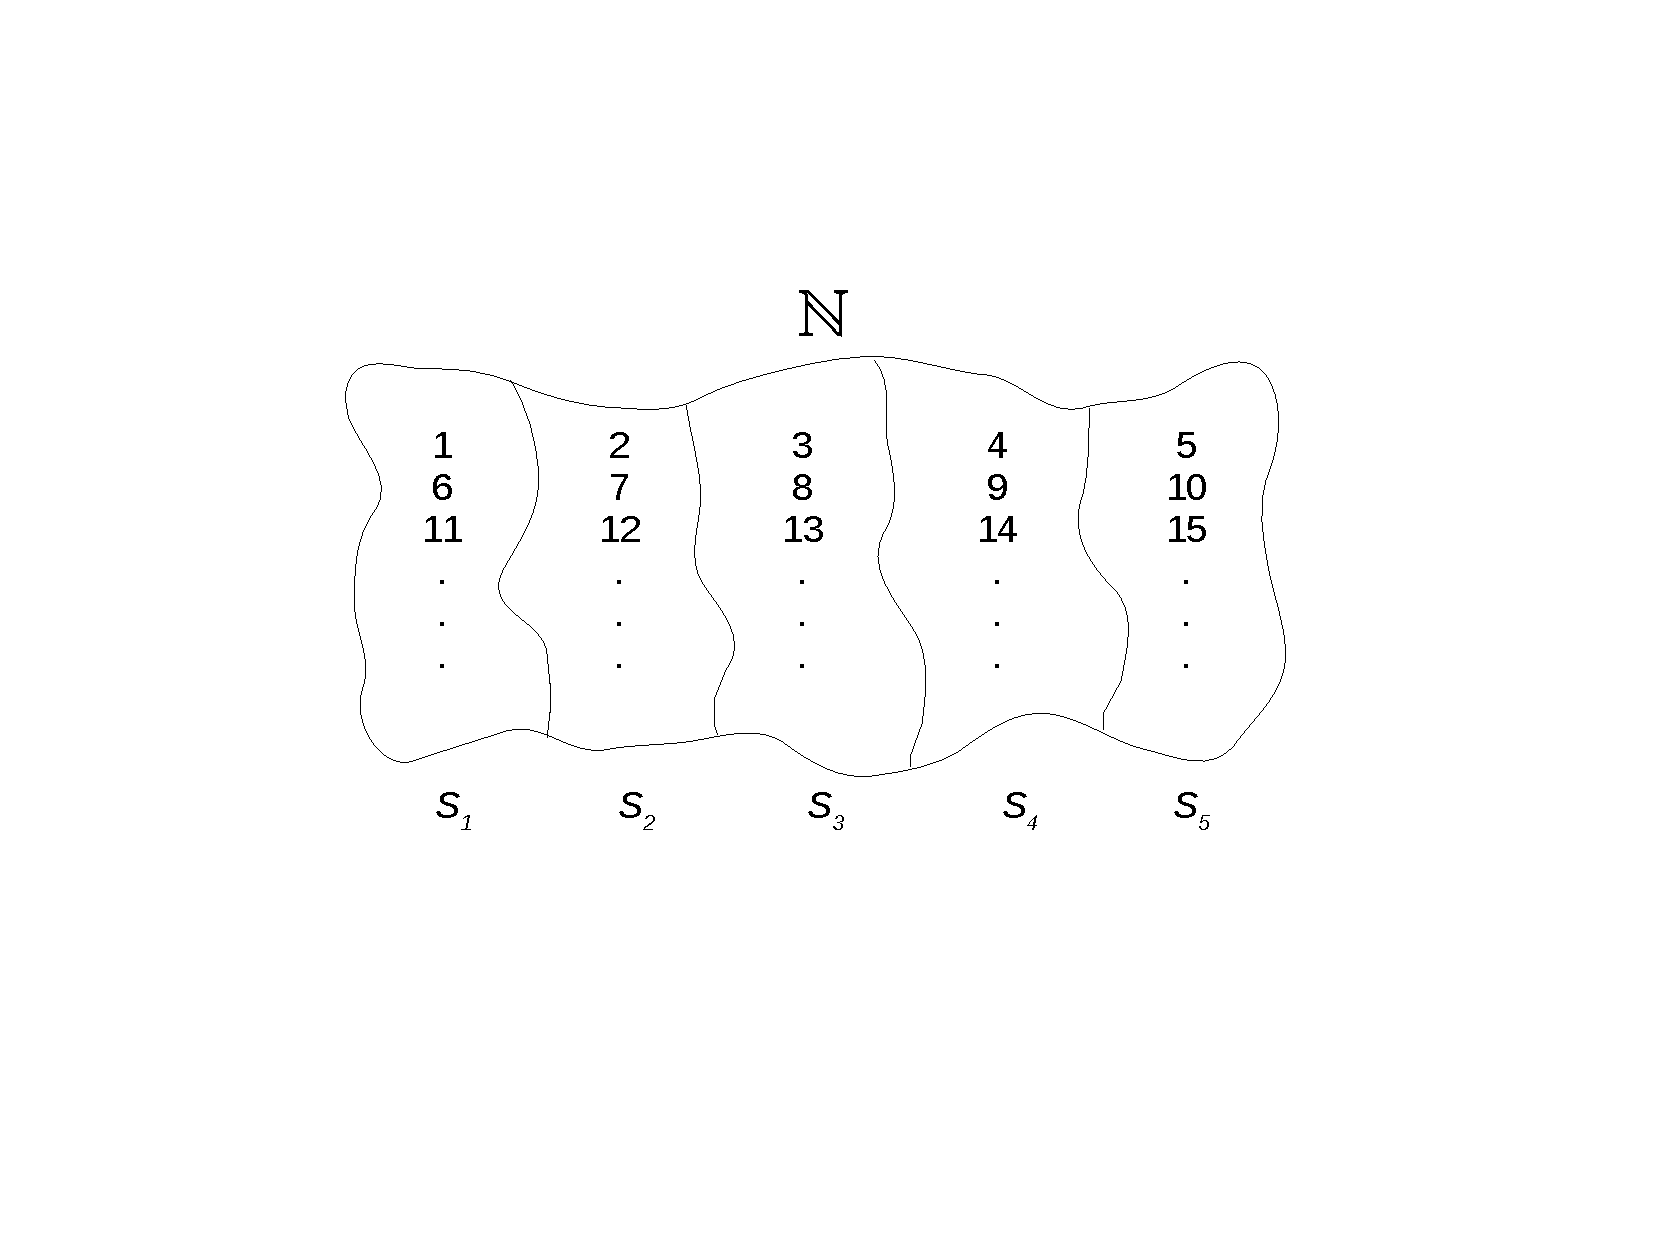
\includegraphics[width=13cm,trim={3cm 6.5cm 3cm 4cm},clip]{./figuras/figure25.pdf}
\end{center}
\end{figure}

Existem muitas coisas interessantes sobre estes conjunto para serem notadas. Enquanto em um primeiro momento algu\'em poderia supor que existe um n\'umero infinito deles, mas existem apenas cinco. Tamb\'em, a uni\ao destes cinco conjuntos \'e todo o $\mathbb{N}$, isto \'e dado um elemento $y\in\mathbb{N}$, $y$ \'e um elemento de um destes cinco conjuntos. Para ser mais preciso, existe exatamente um destes conjuntos que tem $y$ como elemento. Isto significa (ceja exemplo \ref{eqexe2} abaixo) que, dados quaisquer dois destes conjuntos, ou eles s\ao iguais, ou eles s\ao disjuntos. Veremos em breve que toda rela\cao de equival\^encia gera conjuntos com essas propriedades, mas primeiro precisamos de algumas defini\cois. 
\begin{definb}
Seja $A$ um conjunto n\ao vazio. Uma {\it parti\cao}\index{Parti\caoi} $\Pi$ de $A$ \'e uma cole\cao de subconjuntos n\ao vazios de $A$ tais que cada elemento de $A$ \'e elemento de exatamente um destes conjuntos.
\end{definb}

Note que se $\Pi$ \'e uma parti\cao de $A$, en\tao os elementos de $\Pi$ s\ao subconjuntos de $A$, chamamaremos eles de os {\it blocos}\index{Parti\caoi!Blocos} de $\Pi$. Vemos ent\aoi, devido a defini\caoi, que se $B$ e $C$ s\ao blocos de $\Pi$, ent\ao ou $B=C$ ou $B\inter C=\varnothing$. Tamb\'em, a uni\ao de todos os elementos de $\Pi$ \'e $A$. Assim, podemos pensar que uma parti\cao de um conjunto como uma separa\cao do conjunto em partes disjuntas, por exemplo, podemos considerar as tr\^es classes de ensino (fundamental, m\'edio e superior) como uma parti\cao do corpo de estudantes. Agora apresentamos alguns exemplos de parti\cois:

\paragraph{{\bf Exemplos}}
\begin{enumerate}[{\bf 1.}]
\item\label{eqexe1} Seja $A$ n\ao vazio. En\tao $\Pi_1=\{\{x\}:x\in A\}$ e $\Pi_2=\{A\}$ s\ao parti\coes de $A$. Em certo senso, $\Pi_1$ \'e aparti\cao mais ``fina'' de $A$ equanto $\Pi_2$ \'e a mais grossa (veja o exerc\ih cio \ref{eqrexcerc3} desta se\caoi).
\item\label{eqexe2} Seja $A=\{1,2,3,4\}$. En\tao $\Pi_1=\{\{1\},\{2,3\},\{4\}\}$ e $\Pi_2=\{\{1,4\},\{2,3\}\}$ s\ao parti\cois de $A$.
\item\label{eqexe3} Referindo-se aos conjuntos $S_i$ mencionados no come\cc o desta se\caoi, vemos que $\{S_1,S_2,S_3,S_4,S_5\}$ \'e uma parti\cao de $\mathbb{N}$.
\end{enumerate}

Exsite uma rela\cao pr\'oxima entre parti\coes e classes de equival\^encia, de fato, dada uma rela\cao de equival\^envia em um conjunto podemos gerar uma parti\caoi (como fizemos com $\mathbb{N}$ acima) e dada uma parti\cao podemos gerar uma rela\cao de equival\^encia. Para ver como isto realmente funciona, precisamos de mais uma defini\caoi:
\begin{definb}
Seja $R$ uma rela\cao de equival\^encia em um conjunto n\ao vazio $A$. Seja $x\in A$. A {\it classe de equival\^encia}\index{Classe de Equiva\^encia} de $x$ m\'odulo $R$, denotada por $[x]_R$ (ou \`as vezes $x/R$), \'e o conjunto de todos os elementos de $A$ que s\ao R-relacionados a $x$. Em s\ih mbolos,
\[
[x]_R=\{y\in A: yRx\}.
\]
O conjunto de tais classes de equival\^encia \'e denotado por $[A]_R$ (ou \`as vezes A/R) e \'e chamado $A$ m\'odulo R. Em s\ih mbolos,
\[
[A]_R=\{[x]_R: x\in A\}.
\]
\end{definb}
Referindo-se mais uma vez ao exemplo do come\cc o da se\caoi, temos:
\begin{equation*}
 \begin{aligned}
{[2]}_R=&\espaco S_2 = \{2,7,12,17,\ldots\},\\
[4]_R=&\espaco [9]_R = [14]_R,\\
[\mathbb{N}]_R=&\espaco \{[1]_R,[2]_R,[3]_R,[4]_R,[5]_R\} = \{[6]_R,[12]_R,[18]_R,[9]_R,[25]_R\}.
 \end{aligned}
\end{equation*}
Para dois exemplos extremos, seja $A$ um conjunto n\ao vazio e seja $R$ a igualdade (isto \'e, $xRy$ se e somente se $x=y$) e seja $S=A\times A$ (tamb\'em uma rela\cao de equival\^encia). En\tao
\begin{equation*}
 \begin{aligned}
&\forall x\in A, [x]_R=\{x\} \textrm { e } [x]_S=A,\\
&[A]_R=\{\{x\}:x\in A\},\\
&[A]_S=\{A\}.
 \end{aligned}
\end{equation*}
No caso de $R$ temos cada classe de equival\^encia contendo exatamente um elemento enquanto que no caso de $S$ existe apenas uma grande classe de equivl\^encia consistindo de todo o conjunto $A$.

Talvez por agora o leitor pensou que $[A]_R$ \'e uma parti\cao de $A$, com as classes de quival\^encia formando os blocos da parti\caoi. Isto \'e, de fato, o caso que demonstraremos em breve, mas antes vamos estabelecer algumas propriedades das classes de equival\^encia.
\begin{teob}\label{relteo1}
Seja $R$ uma rela\cao de equival\^encia em um conjunto n\ao vazio $A$. En\tao
\begin{enumerate}[{\bf a)}]
\item $\forall x\in A, [x]_R\neq\varnothing$.
\item $\forall x,y\in A, [x]_R\inter[y]_R\neq\varnothing$ se e somente se $xRy$.
\item $\forall x,y\in A,[x]_R=[y]_R$ se e somente se $xRy$.
\item $\forall x,y\in A, [x]_R\neq[y]_R$ se e somente se $[x]_R\inter[y]_R=\varnothing.$
\end{enumerate}
\end{teob}
\begin{proof}
 \begin{enumerate}[{\bf a)}]
\item Como $R$ \'e reflexiva, $xRx$ para todo $x\in A$, logo $x\in[x]_R$ e assim $\forall x\in A, [x]_R\neq\varnothing$.
\item Suponha que $z\in [x]_R\inter [y]_R$. Ent\ao $xRz$ e $yRz$. Como $R$ \'e sim\'etrica, $zRy$ e como $R$ \'e tamb\'em transitiva, temos $xRy$ como desejado. Agora, suponha que $xRy$. Ent\ao $y\in[x]_R$. Mas $y\in[y]_R$ tamb\'em, portanto, $[x]_R\inter[y]_R\neq\varnothing$. 
\item Se $[x]_R=[y]_R$ entao $y\in[x]_R$, logo $xRy$. Agora suponha $xRy$ e seja $z\in[x]_R$. Ent\ao $xRz$. Pela simetria de $R$ temos que $yRx$ e pela transitividade de $R$ obtemos $yRz$, logo $z\in[y]_R$ e consequentemente, $[x]_R\subseteq[y]_R$. Um argumento similar (apenas trocar os papeis de $x$ e $y$) mostra que $[y]_R\subseteq[x]_R$, que completa a demonstra\caoi.
\item Segue diretamente dos partes b) e c).
\end{enumerate}
\end{proof}
\\

Terminamos a maior parte do trabalho para mostrar que $[A]_R$ \'e uma parti\caoi de $A$, o que resta est\'a na demonstra\cao do teorema abaixo.
\begin{teob}
Sejam $A$ um conjunto n\ao vazio e $R$ uma rela\cao de equival\^encia em $A$. Ent\ao $[A]_R$ \'e uma parti\cao de $A$.
\end{teob}
\begin{proof}
Devemos mostrar que $[A]_R$ \'e uma cole\cao de subconjuntos n\ao vazios de $A$ que tem a propriedade que cada $x\in A$ \'e um elemento de exatamente uma dos conjuntos de $[A]_R$. Como $[A]_R=\{[x]_R: x\in A\}$ e $x\in[x]_R$ para casa $x\in A$, cada membro de $[A]_R$ \'e n\ao vazio. Isto tamb\'em mostra que cada $x\in A$ \'e um elemento de pelo menos um conjunto, chamado sua pr\'opria classe de equival\^encia. Suponha que existe $y\in A$ tal que $y$ \'e um elemento de dois conjuntos de $[A]_R$. Mas, o teorema anterior \ref{relteo1} mostrou que distintos elementos de $[A]_R$ s\ao disjuntos, o que contradiz o fato de $y$ pertencer a ambas classes de equival\^encia. Portanto, cada elemento de $A$ \'e um elemento de exatamente uma das classes de equival\^encia.
\end{proof}
\\

Assim, vemoa que uma rela\cao de equival\^encia em um conjunto induz uma parti\cao deste conjunto. Este processo tamb\'em funciona a rec\ih proca, isto \'e uma parti\cao de um conjunto induz uma rela\cao de equival\^encia no conjunto. Antes de mostrar este fato precisamos dar um nome para tal rela\caoi. 
\begin{definb}
Seja $\Pi$ uma parti\cao de um conjunto $A$. Definimos a rela\cao $A/\Pi$ (l\^e-se ``$A$ m\'odulo $\Pi$'') em $A$ por $(x,y)\in A/\Pi$ se e somente se existe $B\in\Pi$ tal que $\{x,y\}\subseteq B$. Em palavras, $x$ \'e relacionado a $y$ se e somente se $x$ e $y$ s\ao ambos elementos do mesmo bloco da parti\caoi.
\end{definb}

Referindo-se a $\Pi_2$ do exemplo \ref{eqexe2} dado anteriormente nesta se\caoi, temos
\[
A/\Pi_2=\{(1,1),(1,4),(2,2),(2,3),(3,2),(3,3),(4,1),(4,4)\}.
\]
Uma r\'apida olhada revela que $A/\Pi$ \'e uma rela\cao de equival\^encia, embora, claramente, devemos provar que isto \'e sempre o caso.
\begin{teob}
Seja $\Pi$ uma parti\cao de um conjunto n\ao vazio $A$. Ent\ao $A/\Pi$ \'e uma rela\cao de equival\^encia em $A$.
\end{teob}
\begin{proof}
Seja $\Pi$ uma parti\cao de $A$ e para conveni\^encia de nota\cao vamos escrever $A/\Pi$ como $R$. Devemos mostrar que $R$ \'e reflexiva, sim\'etrica e transitiva. Seja $x\in A$. Como $x$ \'e elemento de algum bloco de $\Pi$, temos $xRx$, logo $R$ \'e reflexiva. Se $xRy$ ent\ao $x$ e $y$ s\ao ambos pertencentes ao mesmo bloco de $\Pi$, ent\ao claramente $y$ e $x$ est\ao no mesmo bloco de $\Pi$ que implica que $yRx$, logo $R$ \'e sim\'etrica. Agora, suponha que $xRy$ e $yRz$. Ent\ao existem $B,C\in\Pi$ tais que $\{x,y\}\subseteq B$ e $\{y,z\}\subseteq C$. Ent\ao vemos que $y\in B\inter C$, logo $B\inter C\neq\varnothing$ e assim $B=C$. Portanto $\{x,z\}\subseteq B$ e $xRz$, logo $R$ \'e transitiva e consequentemente uma rela\cao de equival\^encia. 
\end{proof}
\\

Fechamos agora o c\ih rculo. Uma parti\cao induz uma rela\cao de equival\^encia $A/\Pi$ e uma rela\cao de equival\^encia induz uma parti\cao $[A]_R$. Podemos ainda ver que a parti\cao induzida por uma rel\cao de equival\^encia induz a parti\cao original e vice-versa. Em s\ih mbolos,
\[
[A]_{A/\Pi}=\Pi \textrm{ e } A/[A]_R=R
\]
A demonstra\cao deste fato interessante ser\'a deixada como excerc\ih cio.

\paragraph{Excerc\ih cios \ref{equivalencia}}

\begin{enumerate}[{\bf 1.}]

%excercicio1
\item Sejam $A=\{1,2,3,4,5,6\}$ e $\Pi=\{\{2,4,6\},\{1,5\},\{3\}\}$. Liste os elementos de $A/\Pi$. Encontre $[2]_{A/\Pi}$. 

%excercicio2
\item Seja $\Pi$ uma parti\cao de $A$ e sejam $B,C\in\Pi$. Mostre que se $B\inter C=\varnothing$ ent\ao $B=C$

%excercicio3
\item\label{eqrexcerc3} Sejam $\Pi_1$ e $\Pi_2$ parti\coes de $A$. Dizemos que $\Pi_1$ \'e {\it mais fina}\index{Parti\cao Mais Fina} que $\Pi_2$ e escrevemos $\Pi_1\preceq\Pi_2$ se e somente se $\forall B\in \Pi_1, \exists C\in \Pi_2 \ni B\subseteq C$.
\begin{enumerate}[a)]
\item Se $A=\{1,2,3,4\}$, d\^e exemplos de parti\coes $\Pi_1$ e $\Pi_2$ tais que:
\begin{enumerate}[i.]
\item $\Pi_1\preceq\Pi_2$
\item $\Pi_1$ n\ao \'e mais fino que $\Pi_2$ e $\Pi_2$ n\ao \'e mais fino que $\Pi_1$
\end{enumerate}
\item Sejam $\Pi_1$ e $\Pi_2$ como no exemplo \ref{eqexe1} desta se\cao e seja $\Pi$ qualquer outra parti\cao de $A$. Mostre que $\Pi_1\preceq\Pi\preceq\Pi_2$.
\end{enumerate}

%excercicio4
\item Seja $R$ uma rela\cao de equival\^encia em $A$. Mostre que $A/[A]_R=R$.

%excercicio5
\item Seja $\Pi$ uma parti\cao de $A$. Mostre que $[A]_{A/\Pi}=\Pi$.

%excercicio6
\item Sejam $R_1,R_2$ rela\coes de equival\^encia em A. Dizemos que $R_1$ \'e {\it mais fina}\index{Rela\caoi!Mais fina} que que $R_2$ e escrevemos $R_1\preceq R_2$ se e somente se $R_1\subseteq R_2$.
\begin{enumerate}[a)]
\item Seja $A=\{1,2,3,4\}$. D\^e exemplos de rela\coes de equival\^encia $R_1,R_2$ tais que:
\begin{enumerate}[i)]
\item $R_1\preceq R_2$.
\item $R_1$ n\ao \'e mais fino que $R_2$ e $R_2$ n\ao \'e mais fino que $R_1$. 
\end{enumerate}
\item Seja $A$ um conjunto n\ao vazio e seja $\Omega=\{R: R \textrm{ uma rela\cao de equival\^encia em $A$}\}$. Mostre que $\preceq$ \'e uma ordem parcial em $\Omega$. O que pode ser dito sobre $\preceq$ ser ou n\ao completa?
\item Se $R_1$ e $R_2$ s\ao rela\coes de equival\^encia em uma conjunto n\ao vazio $A$ com $R_1\preceq R_2$, a parti\cao induzida por $R_1$ \'e mais fina que a parti\cao induzida por $R_2$? A rec\ih proca? Ou nada?
\end{enumerate}

%excercicio7
\item\label{eqexcer7} Seja $\Psi$ e $\Pi$ parti\coes de um conjunto n\ao vazio $A$. Definimos
\[
\Psi\star\Pi=\{C\inter D: C\in\Psi, D\in\Pi,C\inter D\neq\varnothing\}.
\]
\begin{enumerate}[a)]
\item Seja $A=\{1,2,3,4,5\}$, $\Psi=\{\{1,2,3\},\{4,5\}\}$ e $\Pi=\{\{1,2\},\{3,4\},\{5\}\}$. Encontre $\Psi\star\Pi$.
\item Mostre que se $\Psi$ e $\Pi$ s\ao parti\coes de um conjunto n\ao vazio $A$, ent\ao $\Psi\star\Pi$ \'e uma parti\cao de $A$.
\item Mostre que $\Psi\star\Pi$ \'e mais fina que $\Psi$ e $\Pi$.
\end{enumerate}

%excercicio8
\item\label{equivalenciaex8} Vamos generalizar a rela\cao de equival\^encia dada no exemplo \ref{relex11} sa se\cao \ref{relacoes} e discutido no come\cc o desta se\caoi. Seja $m\in\mathbb{N}$. Se $x,y\in\mathbb{Z}$, dizemos que $x\equiv y(mod \espaco m)$ se e somente se $m|(x-y)$. [Note que: $x\equiv y(mod \espaco m)$ \'e lido como ``$x$ \'e congruente a $y$ m\'odulo $m$.''] Assim, a rela\cao de equival\^encia mencionada anteiriormente era a congru\^encia m\'odulo $5$. Mais uma nota\caoi, escreveremos as classes de equival\^encia de congru\^encia m\'odulo $m$ como $[x]_m$ e denotaremos o conjunto de todas as classe de equival\^encia m\'odulo $m$ por $\mathbb{Z}_m$. Assim, $\mathbb{Z}_5=\{[1]_5,[2]_5,[3]_5,[4]_5,[5]_5\}$.
\begin{enumerate}[a)]
\item Encontre $[3]_3,[2]_3,[5]_1,$.
\item Encontre duas solu\coes para cada uma das seguintes:
\begin{enumerate}[i)]
\item $x\equiv 3(mod \espaco 14)$.
\item $x^2\equiv 2(mod \espaco 7)$.
\item $x^2\equiv 3(mod \espaco 7)$.
\end{enumerate}
\item Sejam $m,n\in\mathbb{N}$. Mostre que se $m|n$ ent\ao $\mathbb{Z}_n$ \'e mais fina que $\mathbb{Z}_m$.
\item Seja $m\in\mathbb{N}$. Mostre que $\forall x,y,z\in\mathbb{Z}$, $x\equiv y(mod \espaco m)$ implica $x+z\equiv y+z(mod \espaco m)$ e $xz\equiv yz(mod \espaco m)$.
\end{enumerate}

%excercicio9
\item Seja $R$ e $S$ rela\coes de equival\^encia de um conjunto n\ao vazio $A$. Sabemos que $R\inter S$ \'e tamb\'em uma rela\cao de equival\^encia em $A$.
\begin{enumerate}[a)]
\item Seja $x\in A$. Mostre que $[x]_{R\inter S}=[x]_R\inter[y]_S$. 
\item Mostre que $[A]_{R\inter S}=[A]_R\star[A]_S$, onde $\star$ \'e a opera\cao definida no excerc\ih cio \ref{eqexcer7}.
\end{enumerate}

%excercicio10
\item Se $p,q\in\mathbb{N}$, sabemos do excerc\ih cio \ref{eqexcer7} que $\mathbb{Z}_p\star\mathbb{Z}_q$ \'e uma parti\cao de $\mathbb{Z}$.  Existe $n\in\mathbb{N}$ tal que $\mathbb{Z}_p\star\mathbb{Z}_q=\mathbb{Z}_n$? Se for verdade, demonstre o resultado. Se for falso, d\^e um contraexemplo para mostrar que esta parti\cao n\ao \'e desta forma.

%excercicio11
\item {\bf Acredite se quiser:}  

\noindent \textit{\textbf{Conjectura:}} Seja $A$ um conjunto n\ao vazio e $\Pi,\Psi$ parti\coes de $A$. Se $\Pi\preceq\Psi$ e $\Psi\preceq\Pi$ ent\ao $\Pi=\Psi$.

\noindent \textit{\textbf{``Demonstra\caoi'':}} Sejam $\Pi,\Psi$ como acima e seja $B\in\Pi$. Como $\Pi\preceq\Psi$, existe $C\in\Psi $ tal que $B\subseteq C$. Mas como $\Psi\preceq\Pi$, $C\subseteq B$, e portanto $B=C$, logo $B\in\Psi$. Um argumento parecido mostra que $\Psi\subseteq\Pi$ e consequentemente temos $\Pi=\Psi$. 

\noindent \textit{\textbf{``Contraexemplo'':}} Seja $A=\{1,2,3\}$.
\begin{equation*}
 \begin{aligned}
A=&\{1,2,3,4,5\},\\
\Pi=&\{\{1,2\},\{3\},\{4,5\}\},\\
\Psi=&\{\{1\},\{2,3,4\},\{5\}\},\\
 \end{aligned}
\end{equation*}
Ent\ao $\Pi\preceq\Psi$ $(\{3\}\subseteq\{2,3,4\})$ e $\Psi\preceq\Pi$ $(\{1\}\subseteq\{1,2\})$, mas claramente $\Psi\neq\Pi$.
\end{enumerate}
%%%%%%%%%%%%%%%%%%%%%%%%%%%%%%%%%%%%%%%%%%%%%%%%%%%%%%%%%%%%%%%%%%%%%%%%%%%%%%%%%%%%%%%%%%%%

\section{Fun\cois}\label{funcoes}

Uma das ideias mais predominantes em matem\'atica \'e o de fun\caoi. Sem d\'uvida, fomos expostos \`as fun\coes no ensino m\'edio, al\'em disso fun\coes t\^em o papel mais importante c\'aculo. Embora as fun\coes sejam objetos familiares em nosso repert\'orio matem\'atico, o leitor pode se sentir um pouco embara\cc ado para dar uma defini\cao precisa delas. Vamos remediar esta situa\cao imediatamente e descobrir que fun\coes s\ao rela\coes especiais.
\begin{definb}
Seja $f$ uma rela\cao de $A$ em $B$. Ent\ao $f$ \'e uma {\it fun\cao de $A$ em $B$}\index{Fun\caoi} (denotada por $f:A\to B$, se l\^e ``$f$ \'e uma fun\cao de $A$ em $B$'') se e somente se
\begin{enumerate}[{\bf a)}]
\item $\Dom(f)=A$.
\item $\forall x\in A, \forall y,z\in B, [(x,y)\in f\ee (x,z)\in f]\to y=z$.
\end{enumerate}
\end{definb}

Em palavras, a defini\cao acima diz que se $f$ \'e uma rela\cao de $A$ em $B$ tal que para todos $x\in A$ existe exatamente um $y\in B$ tal que $(x,y)\in f$ ent\ao $f$ \'e uma fun\caoi. Condi\cao a) garante que para cada $x\in A$ existe pelo menos um $y$, e a condi\cao b) garante que existir\'a no m\'aximo um, portanto tomadas juntas obtemos ``exatamente uma.''

Se $f$ \'e uma fun\cao de $A$ em $B$ ent\ao a ``propriedade funcional'' de cada $x\in A$ estando relacionado a exatamente um $y\in B$ nos permite usar a nota\cao funcional familiar $y=f(x)$. Se $f$ fosse qualquer das rela\coes ``antigas'' poderia existir v\'arios (ou mesmo nenhum) elementos em $B$ para cada elemento de $A$ e a not\cao $f(x)$ n\ao se referiria a um elemento de $B$, mas ter\ih amos que referir a um subconjunto de $B$.

Como exemplo de algumas rela\coes que s\ao fun\coes e algumas que n\ao s\aoi, sejam
\begin{equation*}
 \begin{aligned}
A=&\{1,2,3,4\},\\
B=&\{1,2,3,4,5\},\\
f=&\{(1,2),(2,3),(3,4),(4,5)\},\\
g=&\{(1,2),(1,3),(2,4),(3,5),(4,5)\},\\
h=&\{(1,1),(2,2),(3,3)\}.
 \end{aligned}
\end{equation*}
Ent\aoi, $f$, $g$ e $h$ s\ao todas rela\coes de $A$ em $B$, mas apenas $f$ \'e uma fun\caoi, $g$ n\ao \'e uma fun\cao pois ambos $(1,2)$ e $(1,3)$ s\ao elementos de $g$ e $h$ n\ao \'e uma fun\cao pois $\Dom(h)=\{1,2,3\}\neq A$. $f$ tem uma forma particularmente simples para a qual podemos descrever com a f\'ormula: $\forall x\in A, f(x)=x+1$. Embora a maioria das fun\coes de pr\'e-c\'aculo e c\'aculo s\ao dadas de uma maneira parecida, n\ao \'e necess\'ario que fun\coes sejam descritas desta forma. De fato, a maioria das fun\coes n\ao podem especificadas em tal forma simples.

Vamos utilizar a seguinte nota\cao e nomes quando estivermos trabalhando com fun\cois. Se $f:A\to B$ e $(x,y)\in f$ ent\ao esvrevemos $y=f(x)$. Note que, o nome da fun\cao \'e $f$ e que $f(x)$ n\ao \'e o nome da fun\cao mas \'e um elemento de $B$, \'e este elemento particular que est\'a relacionado com um certo elemento de $A$, chamado $x$. Se $y=f(x)$ ent\ao dizemos que $y$ \'e a {\it imagem de $x$}\index{Fun\caoi!Imagem} e $x$ \'e a {\i pr\'e-imagem de $y$.}\index{Fun\caoi!Pr\'e-imagem} Tamb\'em observe que devemos dizer ``a'' quando falamos de imagem, mas devemos usar ``uma'' quando falamos de pr\'e-imagens como um elemento de $B$ pode ter v\'arios elementos de $A$ relacionados ao elemento da pr\'e-imagem. Como $f$ \'e uma rela\caoi, podemos trat\'a-la como uma rela\cao e falar de seu dom\ih nio e imagem, composta dela com outras fun\coes e falar de sua inversa. Note tamb\'em que, embora $\Dom(f)=A$ n\ao precisamos que $\Ima(f)=B$, portanto seria conveniente ter um nome para $B$, chamaremos a $B$ de {\it codom\ih nio de $f$}.\index{Fun\caoi!Codom\ih nio} 

Considere o seguinte exemplo: sejam $A=\{1,2,3,4,5\}$ e $B=\{a,b,c,d\}$ e defina $f:A\to B$ como $f(1)=b$, $f(2)=b$, $f(3)=a$, $f(4)=d$ e $f(5)=a$ (veja a figura abaixo):

\begin{figure}[h]
\begin{center}
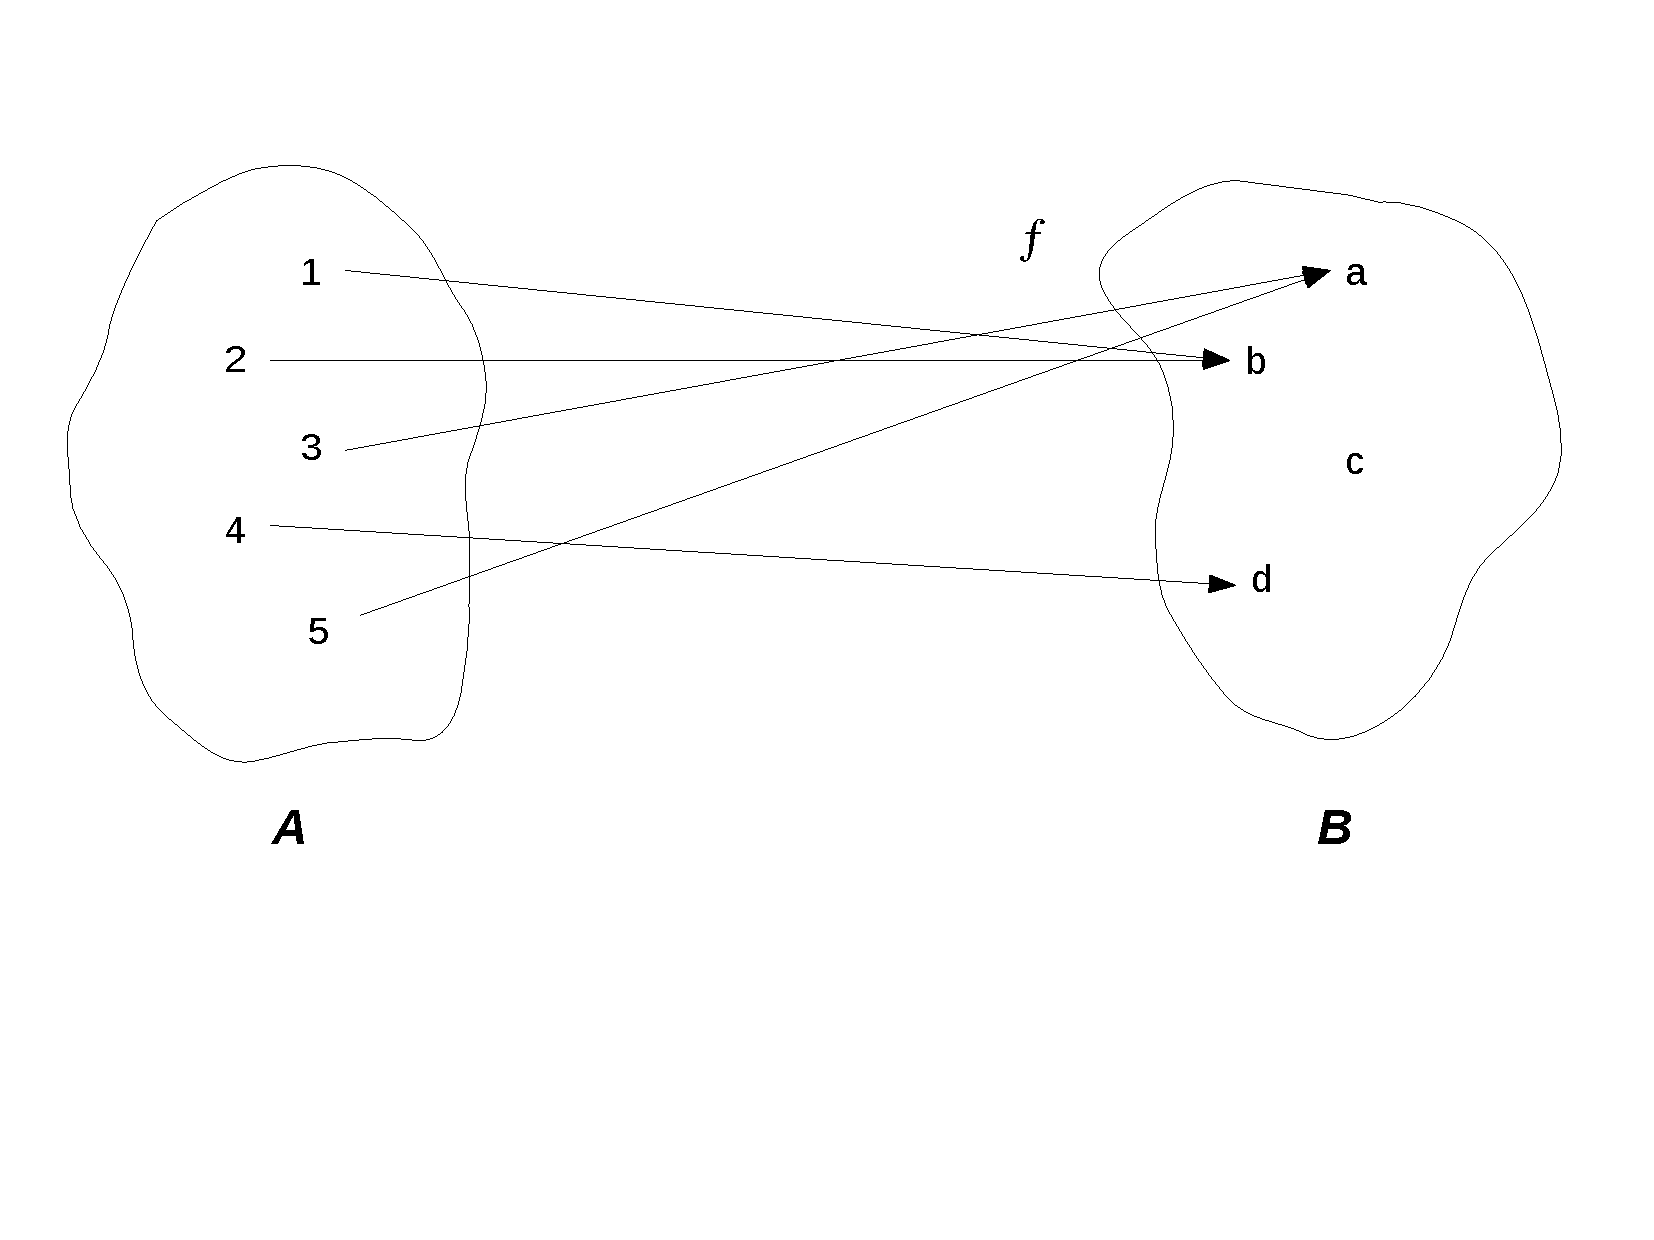
\includegraphics[width=12cm,trim={0.9cm 6.4cm 0.9cm 2.7cm},clip]{./figuras/figure26.pdf}
\end{center}
\end{figure}

Ent\ao a imagem de $2$ \'e $b$, a pr\'e-imagem de $a$ \'e $5$ (outra pr\'e-imagem de $5$ \'e $3$), $c$ n\ao tem pr\'e-imagem.

O seguinte teorema \'e \'util para determinar quando duas fun\coes s\ao iguais:
\begin{teob}
Sejam $f:A\to B$ e $g:A\to B$. Ent\ao $f=g$ se e somente se $\forall x\in A, f(x)=g(x)$.
\end{teob}
\begin{proof}
Primeiro, suponha que $f=g$ e seja $z\in A$. Ent\ao $\exists y\in B\ni (z,y)\in f$. Mas como $f=g$, $(z,y)\in g$. Assim $y=g(z)$ portanto $f(z)=g(z)$.

Agora, suponha que $\forall x\in A, f(x)=g(x)$. Como fun\coes s\ao rela\coes e rela\coes s\ao conjuntos de pares ordenados, para mostrar que $f=g$ devemos mostrar que s\ao iguais como conjuntos de pares ordenados. Para este fim, seja $(w,z)\in f$. Ent\ao $z=f(w)=g(w)$, portanto $(w,z)\in g$ e assim temos que $f\subseteq g$. Trocando $f$ por $g$ no argumento acima, mostramos que $g\subseteq f$. Assim segue que $f=g$. 
\end{proof}
\\

Existem certas propriedades que fun\coes podem ou n\ao ter que aparecem com frequ\^encia suficiente para terem um nome. Algumas destas s\ao dadas abaixo.
\begin{definb}
Seja $f:A\to B$. Ent\ao
\begin{enumerate}[{\bf a)}]
\item Dizemos que $f$ \'e injetora\index{Fun\caoi!Injetora} se e somente se $\forall w,z\in A, f(w)=f(z)$ implica $w=z$. 
\item Dizemos que $f$ \'e sobrejetora\index{Fun\caoi!Sobrejetora} se e somente se $\Ima(f)=B$.
\item Dizemos que $f$ \'e bijetora\index{Fun\caoi!Bijetora} (ou uma correspond\^encia um a um) se e somente se $f$ \'e injetora e sobrejetora.
\end{enumerate}
\end{definb}
A figuras abaixo ilustram as v\'arias possibilidades:

%
%
%
%
%
%
%
%
%
%

Recorde que como fun\coes s\ao rela\cois, elas t\^em inversas que s\ao rela\cois. Assim, podemos falar de inversa de qualquer fun\caoi, mas n\ao h\'a nenhuma raz\ao para esperar que a inversa de uma fun\cao ser\'a uma fun\caoi. Acontece que correspond\^encias um a um (bije\cois) s\ao particularmente importantes porque elas s\ao aquelas fun\coes cujas inversas tamb\'em s\ao fun\cois. Abaixo enunciamos e demonstramos este fato:
\begin{teob}\label{functeo13}
Seja $f:A\to B$. Ent\ao $f^{-1}:B\to A$ se e somente se $f$ \'e uma bije\cao (correspond\^encia um a um).
\end{teob}
\begin{proof}
Primeiro, suponha que $f^{-1}$ seja uma fun\cao de $B$ em $A$. Devemos mostrar que $f$ \'e injetora e sobrejetora. Suponha que $f(x)=f(y)=z$. Isto significa $(x,z)\in f$ e $(y,z)\in f$. Consequentemente, $f^{-1}(z)=x$ e $f^{-1}(z)=y$. Mas $f^{-1}$ \'e uma fun\caoi, portanto $x=y$ e assim $f$ \'e injetora. Para mostrar que $f$ \'e sobrejetora, seja $y\in B$. En\tao como $\Dom(f^{1})=B$, existe $x\in A$ tal que $f^{-1}(y)=x$. Assim $(y,x)\in f^{-1}$ que significa que $(x,y)\in f$ portanto $\Ima(f)=B$.

Agora, suponha que $f$ seja injetora e sobrejetora. Devemos mostrar que $f^{-1}$ \'e uma fun\cao de $B$ em $A$, isto \'e, devemos mostrar que $\Dom(f^{-1})=B$ e que se $(y,x)\in f^{-1}$ e $(y,z)\in f^{-1}$, ent\ao $x=z$. Primeiro, seja $y\in B$. Ent\ao como $f$ \'e sobrejetora, existe $x\in A$ tal que $f(x)=y$ ou $(x,y)\in f$. Assim $(y,x)\in f^{-1}$ portanto $\Dom(f^{-1})=B$. Aogra, suponha qye $(y,x)\in f^{-1}$ e $(y,z)\in f^{-1}$. Ent\ao $f(x)=y$ e $f(z)=y$. Mas como $f$ \'e injetora, isto implica que $x=z$ e consequentemente $f^{-1}$ \'e uma fun\caoi. 
\end{proof}
\\

Vale a pena mencionar que foi a injetividade de $f$ que deu a $f^{-1}$ a propriedade de fun\cao e a sobrejetividade de $f$ gerou o fato que $\Dom(f^{-1})=B$. Devemos ser um pouco cudadosos sobre exatamente o que o teorema diz. Suponha que $f:A\to B$ \'e uma fun\cao injetora mas n\ao uma fun\cao sobrejetora. Ent\ao $f^{-1}$ \'e uma funcaoi, mas n\ao de $B$ em $A$ e sim $f^{-1}:\Ima(f)\to A$.

Poder\ih amos, de fato, ter mostrado um pouco mais sobre $f^{-1}$ no teorema \ref{functeo13}, que $f^{-1}$ \'e tamb\'em uma bije\caoi. Uma demonstra\cao direta \'e poss\ih vel seguindo a demonstra\cao aicma, mas para checar nosso entendimento da nota\cao funcional, considere a seguinte demosntra\caoi:
\begin{teob}\label{functeo14}
Se $f:A\to B$ \'e injetora e sobrejetora ent\ao $f^{-1}:B\to A$ \'e uma bije\caoi.
\end{teob}
\begin{proof}
Usaremos o teorema acima duas vezes: primeiro, o teorema nos diz que $f^{-1}$ \'e uma fun\cao de $B$ em $A$. Agora, trocando os pap\'eis de $f$ e $f^{-1}$, o teorema tamb\'em diz que $(f^{-1})^{-1}$ \'e uma fun\caoi, ent\ao $f^{-1}$ deve ser injetora e sobrejetora. Mas $(f^{-1})^{-1}=f$.
\end{proof}
\\

No excerc\ih cio \ref{funcexerc3} abaixo, o leitor ir\'a demonstrar que a composi\cao de fun\coes \'e novamente uma fun\caoi. Usando este fato, se $f:A\to B$ e $g:B\to C$ ent\ao $(g\bola f):A\to C$. Para ver como nossa nota\cao funcional pode ser usada com a composi\cao de fun\cois, regressemos a deifni\cao de composi\cao de rela\cois. Se $(g\bola f)(x)=z$, ent\ao $(x,z)\in (g\bola f)$ que significa que existe um $y\in B$ tal que $(x,y)\in f$ e $(y,z)\in g$. Consequentemente, $f(x)=y$ e $g(y)=z$. Portanto, $z=g(y)=g(f(x))$ ou $(g\bola y)(x)=g(f(x))$, a nota\cao de composi\cao que usamos em c\'aculo. Agora o leitor pode ver porque escrevemos a composi\cao de rela\coes na ordem que fazemos, de mode que quando escrevemos composi\cao de fun\coes a ordem est\'a de acordo com nossa nota\cao funcional usual. (Digress\aoi: algumas pessoas (principalmente algebristas) contornam esta dificuldade traçando suas nota\coes funcionais, ao inv\'es de $f(x)$, eles escrevem $xf$, que resolve este problema, mas gera outros. Mesmo o mundo inventado das nota\coes matem\'aticas n\ao est\'a livre de dificuldades!)

Como fun\coes s\ao rela\coes podemos compor-las e os resultados que demonstramos para rela\coes continuam v\'alidos. Se $f,g$ s\ao fun\coes com dom\ih nios e imagens adequados, $(g\bola f)^{-1}=f^{-1}\bola g^{-1}$, embora $(g\bola f)^{-1}$, $f^{-1}$ e $g^{-1}$ possam n\ao serem fun\cois. O teorema \ref{functeo14} nos diz que se $f,g$ s\ao bije\cois, ent\ao $f^{-1}$ e $g^{-1}$ ser\ao fun\cois. Para completar nossa vis\ao sobre esse tema, provaremos mais dois teoremas sobre composi\cao de inversas de fun\cois.
\begin{teob}\label{functeo15}
Sejam $f:A\to B$ e $g:B\to C$ bije\cois. Ent\ao $g\bola f:A\to C$ \'e uma bije\caoi. 
\end{teob}
\begin{proof}
Contando com os resultados do excerc\ih cio \ref{funcexerc3} abaixo, assumiremos que $g\bola f$ \'e uma fun\cao de $A$ a $C$, portanto precisamos apenas mostrar que \'e uma bije\caoi. Primeiro, suponha que exista $x,y\in A$ tais que $g\bola f(x)=g\bola f(y)$. Assim, $g(f(x))=g(f(y))$. Mas $g$ \'e injetora, portanto $f(x)=f(y)$. Agora, o fato que $f$ \'e injetora nos diz que $x=y$, logo $g\bola f$ \'e injetora. Para mostrar que $g\bola f$ \'e sobrejetora, seja $z\in C$. Como $g$ \'e sobrejetora, existe $y\in B$ tal que $g(y)=z$. Mas $f$ \'e sobrejetora ent\ao existe $x\in A$ tal que $f(x)=y$. Assim, $z=g(y)=g(f(x))=g\bola f(x)$, logo $g\bola f$ \'e sobrejetora.
\end{proof}
\\

A demonstra\cao acima \'e uma t\ih pica demosntra\cao que mostra que uma certa fun\cao \'e injetora e sobrejetora. Para ter certeza que entendemos a forma deste tipo de demonstra\caoi, vamos dar uma olhada mais de perto. Suponha que $f:A\to B$. Uma demonstra\cao direta para mostrar que $f$ \'e injetora seria tomar a forma: Seja $x,y\in A$, com $f(x)=f(y)$.
\\
\ldots
\\ 
``alguma coisa ou outra dependendo de $f$''
\\
\ldots
\\
portanto $x=y$ e assim $f$ \'e injetora.

A demonstra\cao por contrapositiva seria da forma: Sejam $x,y\in A$, com $x\neq y$.
\\
\ldots
\\ 
``alguma coisa ou outra dependendo de $f$''
\\
\ldots
\\
portanto $f(x)\neq f(y)$ e assim $f$ \'e injetora.

A demonstra\cao direta para mostrar que $f$ \'e sobrejetora se pareceria como: Seja $y\in B$.
\\
\ldots
\\ 
``alguma coisa ou outra dependendo de $f$''
\\
\ldots
\\
portanto existe $x\in A$ tal que $f(x)=y$ e $f$ \'e sobrejetiva.

Resumo: para mostrar que $f$ \'e injetora, devemos mostrar que elementos distintos em um dom\ih nio t\^em imagens distintas e para mostrar que $f$ \'e sobrejetora, devemos mostrar que todos elementos de $B$ t\^em uma pr\'e-imagem.

Como exemplo, vamos mostrar que $f:\mathbb{R}\to\mathbb{R}$ dada por $f(x)=ax+b$, com $a\neq 0$ \'e uma bije\caoi. Primeiro, uma demonstra\cao direta que $f$ \'e injetora. Sejam $x,y\in\mathbb{R}$ com $f(x)=f(y)$. Ent\ao $ax+b=ay+b$ que implica que $ax=ay$. Como $a\neq 0$, temos $x=y$ e portanto $f$ \'e injetora. A demonstra\cao por contrapositiva deste fato seria: Sejam $x,y\in\mathbb{R}$ com $x\neq y$. Ent\ao como $a\neq 0$, $ax\neq ay$ portanto temos que $ax+b\neq ay+b$, logo $f(x)\neq f(y)$. Para mostrar que $f$ \'e sobrejetora, seja $z\in\mathbb{R}$. Ent\ao $(z-b)/a$ \'e tamb\'em um elemento de $\mathbb{R}$ (pois $a\neq 0$) e
\[
f\left(\frac{z-b}{a}\right)= a\left(\frac{z-b}{a}\right)+b=z-b+b=z.
\] 
portanto $f$ \'e sobrejtora. Devemos notar que a escolha de $(z-b)/a$ n\ao veio do nada, foi o resultado de resolver d equa\cao $f(x)=ax+b=z$ para $x$.
\begin{teob}\label{functeo16}
Sejam $f:A\to B$ e $g:B\to C$ bije\cois. Ent\ao $(g\bola f)^{-1}:C\to A$ e $\forall x\in C$, $(g\bola f)^{-1}(x)=(f^{-1}\bola g^{-1})(x)=f^{-1}(g^{-1}(x))$. 
\end{teob}
\begin{proof}
J\'a fizemos a maior parte do trabalho, assim devemos apenas fazer algumas observa\cois. Primeiro, como $f$ e $g$ s\ao bije\cois, $g\bola f$ tamb\'em \'e uma bije\caoi, portanto $(g\bola f)^{-1}$ \'e uma fun\cao de $C$ em $A$. Das rela\coes sabemos que, $(g\bola f)^{-1}=(f^{-1}\bola g^{-1}$ e como $f^{-1}$ e $g^{-1}$ s\ao fun\coes tamb\'em, o resultado segue.
\end{proof}
\\

Note que a rela\cao identidade em $A$, $I_A$, \'e uma fun\cao de $A$ em $A$ a qual chamaremos de {\it fun\cao identidade}.\index{Fun\caoi!Identidade} Usando nossa nota\cao funcional, $I_A(x)=x$ para todo $x\in A$. A raz\ao para este nome (e para o nome inversa) ficar\'a mais claro no r\'oximo teorema.
\begin{teob}\label{functeo17}
Seja $f:A\to B$. Ent\aoi
\begin{enumerate}[{\bf a)}]
\item $f\bola I_A=f$. 
\item $I_B\bola f=f$.
\item Se $f$ \'e uma bije\cao ent\ao $f^{1}\bola f=I_A$ (ou $\forall x\in A, f^{1}(f(x))=x$) e $f\bola f^{1}=I_B$ (or $\forall x\in B, f(f^{1}(x))=x$).
\end{enumerate}
\end{teob}
\begin{proof}
Itens a) e b) seguem facilmente, para isso suponha que $x\in A$. Ent\ao $f\bola I_A(x)=f(I_A(x))=f(x)$ e $I_B\bola f(x)=I_B(f(x))=f(x)$. Para c), primeiro observe que como $f$ \'e uma bije\caoi, $f^{-1}$ \'e uma fun\caoi, logo $f(x)=y$ se e somente se $f^{-1}(y)=x$. Agora, seja $x\in A$ e suponha que $f(x)=y$. En\tao $(f^{-1}\bola f)(x)=f^{-1}(f(x))=f^{-1}(y)=x=I_A(x)$. Para a segunda asser\caoi, seja $x\in B$ e suponha que $f^{-1}(x)=y$. Assim, $(f\bola f^{-1})(x)=f(f^{-1}(x))=f(y)=x=I_B(x)$.
\end{proof}
\\

\paragraph{Excerc\ih cios \ref{funcoes}}

\begin{enumerate}[{\bf 1.}]

%excercicio1
\item Seja $A=\{1,2,3,4,5,6\}$ e seja $f:A\to A$ dada por 
\begin{equation*}
 f(x)=\left\{ \begin{array}{lc}
x+1, & \textrm{ se $x\neq 6$;} \\
1,    & \textrm{ se $x=    6$.} \\
\end{array}\right.   
\end{equation*}
\begin{enumerate}[a)]
\item Encontre $f(3)$, $f(6)$, $f\bola f(3)$, $f(f(2))$. 
\item Encontre a pr\'e-imagem de $2$ e $1$.
\item Mostre que $f$ \'e bijetora.
\end{enumerate}

%excercicio2
\item Mostre que $f:\mathbb{R}\to\mathbb{R}$ dad por $f(x)=x^3$ \'e injetora e sobrejetora, enquanto que $g:\mathbb{R}\to\mathbb{R}$ dada por $g(x)=x^2-1$ n\ao \'e injetora nem sobrejetora. 

%excercicio3
\item\label{funcexerc3} Suponha $f:A\to B$ e $g:B\to C$. Mostre que $g\bola f:A\to C$.

%excercicio4
\item \begin{enumerate}[a)]
\item Sejam $A,B$ e $f:A\to B$ dados por:
\begin{equation*}
 \begin{aligned}
A=&\{1,2,3,4\},\\
B=&\{1,2,3,\},\\
f=&\{(1,3),(2,1),(3,1),(4,2)\}.
 \end{aligned}
\end{equation*}
Encontre $f^{-1}\bola f$.
\item Sejam $A,B$ conjuntos n\ao vazios e $f:A\to B$. Mostre que $f^{-1}\bola f$ \'e uma rela\cao de equival\^encia em $A$. (Note que $f^{-1}$ pode ou n\ao ser uma fun\caoi). Tamb\'em mostre que $[x]_{f^{-1}\bola f}=\{y: f(x)=f(y)\}$.
\end{enumerate}

%excercicio5
\item Seja $f:A\to B$. Prove que
\begin{enumerate}[a)]
\item $f$ \'e injetora se e somente se existe $g:B\to A$ tal que $g\bola f=I_A$.
\item $f$ \'e sobrejetora se e somente se existe $g:B\to A$ tal que $f\bola g=I_B$.
\item $f$ \'e sobrejetora se e somente se $f\bola f^{-1}=I_B$.
\end{enumerate}

%excercicio6
\item Sejam $f:A\to B$ e $g:B\to A$. Mostre que se $g\bola f=I_A$ e $f\bola g=I_B$ ent\ao $f$ \'e uma bije\cao e $g=f^{-1}$

%excercicio7
\item Seja $R$ uma rela\cao de equival\^encia em um conjunto n\ao vazio $A$. Definimos a rela\cao $\alpha$ de $A$ em $[A]_R$ por
\[
\alpha=\{(x,[x]_R): x\in A\}.
\]
\begin{enumerate}[a)]
\item Mostre que $\alpha:A\to [A]_R$.
\item Mostre que $\alpha$ \'e sobrejetora.
\item Sob quais condi\coes $\alpha$ ser\'a injetora?
\end{enumerate}

%excercicio8
\item Seja $f:A\to A$. Suponha que $f$ tamb\'em seja uma rela\cao de equival\^encia. O que podemos dizer sobre $f$? 

%excercicio9
\item Sejam $f:A\to B$ e $g:A\to B$. Demonstre ou d\^e contraexemplos para as seguintes conjecturas:
\begin{enumerate}[a)]
\item $f\uni g:A\to B$.
\item $f\inter g:A\to B$.
\item $f\uni g:A\to B$ implica $f=g$.
\item $f\inter g:A\to B$ implica $f=g$.
\end{enumerate}

%excercicio10
\item Seja $f:A\to B$ e $g:C\to D$, com $A\inter C=\varnothing$. [Para refrescar sua mem\'oria sobre restri\cois, veja o excerc\ih cio \ref{relexer13} da se\cao \ref{relacoes}]. 
\begin{enumerate}[a)]
\item Mostre que $f\uni g:A\uni C\to B\uni D$.
\item Mostre que $f\uni g|_A=f$ e $f\uni g|_C=g$. 
\end{enumerate}

%excercicio11
\item Seja $f:\mathbb{R}\to\mathbb{R}$ definida por $f(x)=\textrm{sen}(x).$
\begin{enumerate}[a)]
\item Mostre que $f$ n\ao \'e injetora.
\item Mostre que $f|_{[\pi/2,\pi/2]}$ \'e injetora.
\end{enumerate}

%excercicio12
\item Seja $A$ um conjunto n\ao vazio e seja 
\[
\Psi=\{\phi: \phi \textrm{ \'e uma parti\cao de } A\}.
\] 
Lembre-se que $\preceq$ (mais fino que) \'e uma rela\cao de ordem parcial em $\Psi$. Seja
\[
\Re=\{R: R \textrm{ \'e uma rela\cao de equival\^encia em } A\}.
\]
Sabemos que existe uma bije\cao entre os elementos de $\Psi$ e $\Re$, assim denotemos a rela\cao de equival\^encia associada com a parti\cao $\theta$ por $R_{\theta}$. Definimos s rela\cao $\sqsubseteq$ em $\Re$ por
\[
R_{\phi}\sqsubseteq R_{\theta} \textrm{ se e somente se } \phi \preceq \theta.
\]
\begin{enumerate}[a)]
\item Mostre que $\sqsubseteq$ \'e uma ordem parcial em $\Re$.
\item Mostre (ou d\^e um contraexemplo):
\[
R_{\phi}\sqsubseteq R_{\theta} \textrm{ se e somente se } R_{\phi}\subseteq R_{\theta}.
\]
\end{enumerate}

%excercicio13
\item Suponha que $f:A\to B$ e $g:B\to C$, onde $A,B$ e $C$ s\ao conjuntos n\ao vazios. Demonstre ou d\^e contraexemplos para as seguintes conjecturas:
\begin{enumerate}[a)]
\item $g\bola f$ bije\cao implica que $f$ \'e injetora. 
\item $g\bola f$ bije\cao implica que $f$ \'e sobrejetora.
\item $g\bola f$ bije\cao implica que $g$ \'e sobrejetora.
\item $g\bola f$ bije\cao implica que $g$ \'e injetora.
\end{enumerate}

%excercicio14
\item Seja $f:A\to B$, com $R$ uma ordem total estrita em $A$ e $S$ uma ordem total estrita em $B$. Dizemos que $f$ \'e {\it monot\^onica}\index{Fun\caoi!Monot\^onica} se e somente se $\forall x,y\in A,$ $xRy$ implica $f(x)Sf(y)$.
\begin{enumerate}[a)]
\item Com a ordem usual ($<$) em $\mathbb{R}$, de um exemplo de uma fun\cao que seja monot\^onica.
\item Com a ordem usual ($<$) em $\mathbb{R}$, de um exemplo de uma fun\cao que n\ao seja monot\^onica.
\item Se $f:A\to B$ \'e monot\^onica, mostre que $f$ \'e injetora.
\end{enumerate}

%excercicio15
\item {\bf Acredite se quiser:}  

\noindent \textit{\textbf{Conjectura:}} Seja $f:A\to B$ e seja $R$ uma ordem total estrita em $A$. Definimos a rela\cao $S$ em $B$ por
\[
xSy \leftrightarrow \exists a,b\in A \ni aRb\ee f(a)=x,f(b)=y.
\]
Ent\ao $S$ \'e uma ordem parcial estrita.

\noindent \textit{\textbf{``Demonstra\caoi'':}} Suponha que $f$ e $ R$ s\ao como acima e $S$ \'e definida como indicado. Seja $x\in B$ com $xSx$. Mas isto significa que existe $a\in A$ tal que $f(a)=x$. Assim $aRa$, que \'e imposs\ih vel, pois $R$ \'e irreflexiva, portanto $S$ \'e irreflexiva. Agora, suponha $x,y,z\in B$ com $xSy$, $ySz$. Ent\ao existem $a,b,c\in A$ tais que $f(a)=x$, $f(b)=y$ e $f(c)=z$ e $aRb$ e $bRc$. Como $R$ \'e transitiva, $aRc$ e portanto $xSz$, logo $S$ \'e transitiva.

\noindent \textit{\textbf{``Contraexemplo'':}} Sejam $A=\{1,2,3\}$, $B=\{1,2,3,4\}$ e $f:A\to B$ dada por $f(1)=1$, $f(2)=1$ e $f(3)=4$. Suponha,
\[
R=\{(1,2),(2,3),(1,3)\}
\]
Ent\ao $S=\{(1,2),(1,4)\}$, que \'e transitiva mas n\ao irreflexiva.

%excercicio16
\item {\bf Acredite se quiser:}  

\noindent \textit{\textbf{Conjectura:}} Seja $f:A\to B$ e $g:B\to A$. Se $g\bola f=I_A$ ent\ao $g=f^{-1}$.

\noindent \textit{\textbf{``Demonstra\caoi'':}} Sejam $f,g$ como acima e seja $x\in B$. Suponha que $y\in A$ \'e tal que $(x,y)\in g$. Seja $x\in B$ tal que $(y,z) \in f$. Como $g\bola f=I_A$, $(x,y)\in g$. Mas $(x,y)\in g$ e $g$ \'e uma fun\caoi, portanto $x=z$. Assim, $(x,y)\in f^{-1}$, logo $g\subseteq f^{-1}$. Agora suponha que $(x,y)\in f^{-1}$. Ent\ao $(y,x)\in f$. Como $g\bola f=I_A$, $(x,y)\in g$, logo $f^{-1}\subseteq g$ e portanto temos que $g=f^{-1}$.

\noindent \textit{\textbf{``Contraexemplo'':}} Sejam $A=\{1,2,3\}$, $B=\{1,2,3,4\}$ com
\[
f=\{(1,2),(2,1),(3,3)\}
\]
\[
g=\{(2,1),(1,2),(3,3),(4,3)\}
\]
Ent\ao $g\bola f=I_A$ mas $g\neq f^{-1}$, pois $(4,3)\in g$.

%excercicio17
\item {\bf Acredite se quiser:}  

\noindent \textit{\textbf{Conjectura:}} Seja $f:A\to B$. Se $f^{-1}\bola f=I_A$ ent\ao $f$ \'e injetora.

\noindent \textit{\textbf{``Demonstra\caoi'':}} Suponha que $f$ \'e como descrito acima e $x,y\in A$ com $f(x)=f(y)=z$. Ent\ao $f^{-1}(z)=x$ e $f^{-1}(z)=y$. Mas $f^{-1}$ \'e uma fun\caoi, portanto $x=y$ e assim $f$ \'e injetora.

\noindent \textit{\textbf{``Contraexemplo'':}} Sejam $A=\{a,b,c\}$ e $B=\{1,2,3\}$ com $f(a)=1$, $f(b)=2$ e $f(c)=2$. En\tao $f^{-1}=\{(1,a),(2,b),(2,c)\}$ mas $f$ n\ao \'e injetora.
\end{enumerate}
%%%%%%%%%%%%%%%%%%%%%%%%%%%%%%%%%%%%%%%%%%%%%%%%%%%%%%%%%%%%%%%%%%%%%%%%%%%%%%%%%%%%%%%%%%%%

\section{Mais Fun\cois}\label{mfuncoes}

Podemos extender a ideia de fun\cao de uma forma natural de elementos individuais do dom\ih nio em subconjuntos do dom\ih nio, isto \'e, $f:A\to B$ pode ser extendido para $f:\mathbb{P}(A)\to \mathbb{P}(B)$.
\begin{definb}
Seja $f:A\to B$. Se $C\subseteq A$ ent\ao definimos $f(C)=\{f(x): x\in C\}$. Se $D\subseteq B$ en\tao $f^{-1}(D)=\{x: f(x)\in D\}$. $f(C)$ \'e chamada a imagem de $C$ e $f^{-1}(D)$ \'e chamada a pr\'e-imagem de $D$.
\end{definb}

Por exemplo, seja $f:A\to B$ onde $A=\{1,2,3,4\}$, $B=\{1,3,5\}$ e $f$ dada por $f(1)=1$, $f(2)=1$, $f(3)=5$ e $f(4)=5$. Ent\ao
\begin{equation*}
 \begin{aligned}
f(\{1,3\})=&\{1,5\},\\
f(\{1,2\})=&\{1\},\\
f^{-1}(\{1\})=&\{1,2\},\\
f^{-1}(\{4\})=&\varnothing.
 \end{aligned}
\end{equation*}
Note que at\'e agora definimos alguns conjuntos: com $A,B,f,C,D$ como acima, $f(C)$ \'e um subconjunto de $B$ e $f^{-1}(D)$ \'e um subconjunto de $A$. Entretanto, podemos utilizar estas defini\coes de uma forma natural para definir algumas fun\coes (com o mesmo nome)
\[
f:\mathbb{P}(A)\to \mathbb{P}(B),
\]
\[
f^{-1}:\mathbb{P}(B)\to \mathbb{P}(A).
\]
Estas duas fun\coes induzidas por conjuntos t\^em muitas propriedades importantes (incluindo o fato de que elas s\ao fun\cois!), que em sua maioria ser\ao deixadas para os excerc\ih cios, mas provaremos uma aqui para dar uma dica de como s\ao estas demonstra\cois.
\begin{teob}
Seja $f:A\to B$ e sejam $C\subseteq D \subseteq B$. Ent\ao
\[
f^{-1}(C)\subseteq f^{-1}(D).
\]
\end{teob}
\begin{proof}
Seja $x\in f^{-1}(C)$. Ent\ao $x\in A$ e $f(x)\in C$. Como $C\subseteq D$, $f(x)\in D$. Mas isto significa que $x\in f^{-1}(D)$.
\end{proof}
\\

Todas as nossas familiares opera\coes aritm\'eticas ($+$, $-$, $\cdot$ e $\div$) s\ao funcois, assim como todos os conectivos l\'ogicos ($\ee$, $\ou$, $\rightarrow$ e $\leftrightarrow$) e todas opera\coes de conjuntos ($\inter$, $\uni$ e $-$). Temos um nome especial para fun\coes deste tipo:
\begin{definb}
Seja $A$ um conjunto. $\bullet$ \'e chamada {\it opera\cao bin\'aria}\index{Opera\cao Bin\'aria} em $A$ se e somente se 
\[
\bullet :A\times A\to A.
\]
\end{definb}

Assim vemos que a oper\cao bin\'aria em $A$ associa cada par de elementos de $A$ a um elemento de $A$. Por causa disso iremos nos afastarde nossa nota\cao funcional usual e escrever:
\[
a\cdot b=c \textrm{ ao inv\'es de } \cdot((a,b))=c.
\]

Por exemplo, com $+:\mathbb{R}\times\mathbb{R}\to\mathbb{R}$ (adi\cao de n\'umeros reais), escrevemos $2+3=5$ ao inv\'es de $+((2,3))=5$.

Existem muitas propriedades que as opera\coes bin\'arias podem ou n\ao ter:
\begin{definb}
Seja $\bullet$ uma opera\cao bin\'aria em um conjunto $A$. Ent\aoi:
\begin{enumerate}[{\bf a)}]
\item Dizemos que $\bullet$ \'e {\it comutativa}\index{Opera\cao Bin\'aria!Comutativa} se e somente se $\forall a,b\in A, a\bullet b=b\bullet a$.
\item Dizemos que $\bullet$ \'e {\it associativa}\index{Opera\cao Bin\'aria!Associativa} se e somente se $\forall a,b,c\in A, a\bullet(b\bullet c)=(a\bullet b)\bullet c$.
\item Dizemos que $e\in A$ \'e uma {\it identidade}\index{Opera\cao Bin\'aria!Identidade} para $\bullet$ se e somente se $\forall a\in A, a\bullet e=e\bullet a=a$.
\item Se $e$ \'e uma identidade para $\bullet$ e $x\in A$, dizemos que $x$ \'e {\it invert\ih vel}\index{Opera\cao Bin\'aria!Elemento Inverso} se e somente se $\exists y\in A \ni x\bullet y=y\bullet x=e$. Tal $y$ \'e chamado um {\it inverso} de $x$.
\item Dizemos que $a\in A$ \'e {\it idempotente}\index{Opera\cao Bin\'aria!Elemento Idempotente} para $\bullet$ se e somente se $a\cdot a=a$.
\end{enumerate}
\end{definb}

Alguns exemplos destas propriedades, $+$ em $\mathbb{R}$ \'e comutativa, associativa, tem $0$ como identidade e todo elemento \'e invert\ih vel (o inverso de $x$ \'e $-x$). O \'unico elemento idempotente \'e $0$. Por outro lado, $-$ em $\mathbb{R}$ n\ao \'e comutativo, n\ao \'e associativo, n\ao tem identidade e o \'unico elemento idempotente \'e $0$. $\uni$ em $\mathbb{P}(A)$ para algum conjunto $A$ \'e comutativo, associativo, $\varnothing$ \'e a identidade e cada elemento \'e idempotente.

Vamos demonstrar alguns poucos teoremas envolvendo oper\coes bin\'arias e deixar alguns outros para os ecerc\ih cios.
\begin{teob}
Seja $\bullet$ uma opera\cao bin\'aria em $A$. Ent\ao existe no m\'aximo uma identidade para $\bullet$.
\end{teob}
\begin{proof}
Suponha que $e$ e $e'$ s\ao ambos identidades para $\bullet$. Ent\ao
\[
e=e\bullet e'=e'
\]
Assim $e=e'$ e $\bullet$ pode ter no m\'aximo uma identidade.

\noindent [Nota: A primeira igualdade \'e v\'alida pois $e'$ \'e uma identidade e a segunda \'e v\'alida porque $e$ \'e uma identidade.] 
\end{proof}
\\

\begin{teob}\label{functeo20}
Se $\bullet$ \'e uma opera\cao bin\'aria associativa com identidade $e$ em $A$ e $x\in A$, ent\ao $x$ tem no m\'aximo um inverso.
\end{teob}
\begin{proof}
Suponha que $x\in A$ tem dois inversos, que chamaremos de $y$ e $y'$. Ent\ao
\[
x\bullet y=y\bullet x=e
\]
e
\[
x\bullet y'=y'\bullet x=e
\]
Assim,
\[
y=y\bullet e=y\bullet(x\bullet y')=(y\bullet x)\bullet y'=e\bullet y'=y'.
\]
\end{proof}
\\

Em virtude dos teoremas acima podemos falar em ``a'' identidade e ``o'' inverso de um elemento (se tais existem).

A \'ultima ideia que gostar\ih amos de introduzir nesta se\cao pode, de alguma forma, ser sutil, mas o esfor\cc o para entende-la ser\'a recompensado no futuro (por exemplo, quando o leitor estiver estudando em \'algebra o ``teorema fundamental de homomorfismos de grupos'').
\begin{teob}\label{functeo21}
Seja $f:A\to B$. Definimos a rela\cao $R$ em $A$ por $xRy$ se e somente se $f(x)=f(y)$. Ent\ao $R$ \'e uma rela\cao de equival\^encia em $A$ e consequentemente $[A]_R$ \'e uma parti\cao de $A$. Definimos duas novas fun\cois:
\begin{equation*}
 \begin{aligned}
&\alpha:A\to[A]_R \textrm{ por } \alpha(x)=[x]_R,\\
&f^{\ast}:[A]_R\to B \textrm{ por } f^{\ast}([x]_R)=f(x). 
 \end{aligned}
\end{equation*}
Ent\ao $f^{\ast}$ \'e injetora e $f=f^{\ast}\bola\alpha.$
\end{teob}
\begin{proof}
Ser\'a \'util manter a figura abaixo na mente durante nosso trabalho na demonstra\caoi.

\begin{figure}[h]
\begin{center}
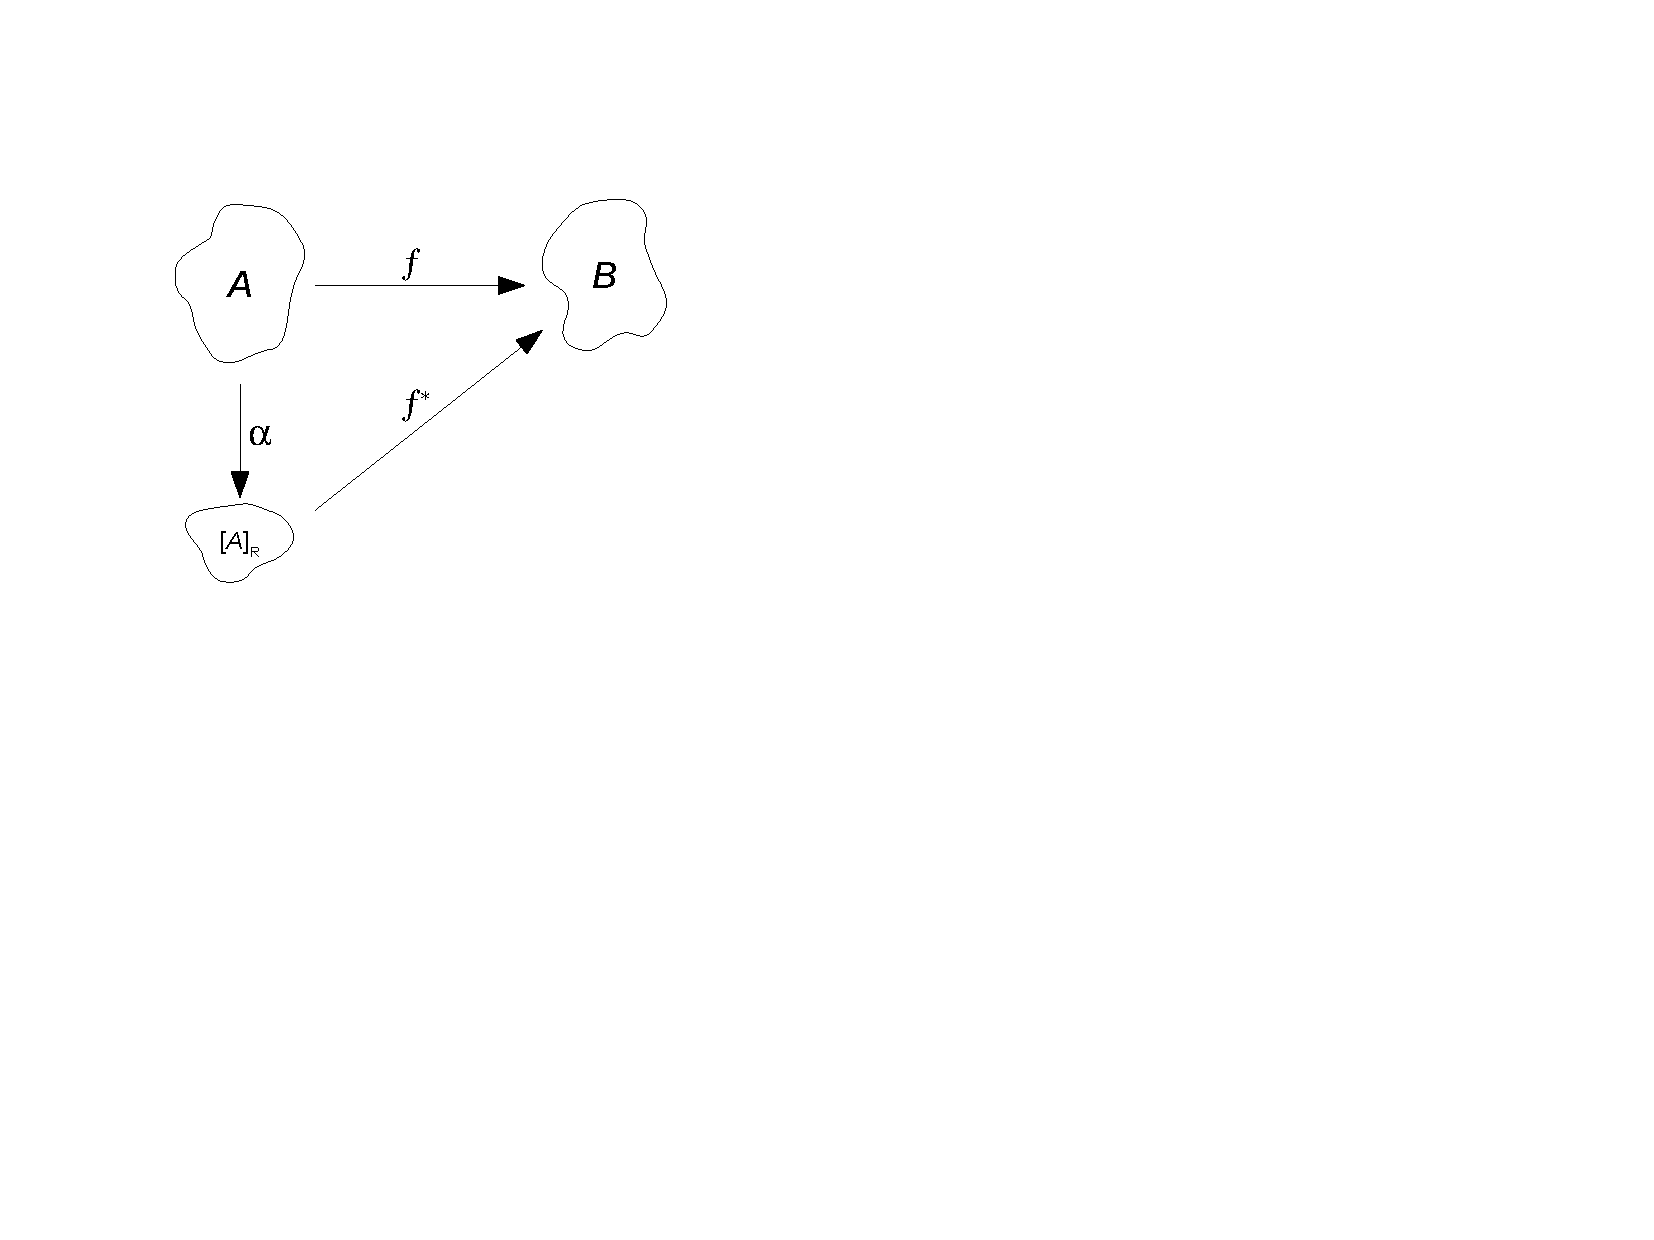
\includegraphics[width=15cm,trim={1.3cm 11.1cm 16cm 2.3cm},clip]{./figuras/figure28.pdf}
\end{center}
\end{figure}

Devemos observar que h\'a quatro coisas que devem ser provadas:
\begin{enumerate}[{\bf a)}]
\item $R$ \'e uma rela\cao de equival\^encia.
\item $f^{\ast}$ \'e uma fun\caoi.
\item $f^{\ast}$ \'e injetora.
\item $f=f^{\ast}\bola\alpha$. 
\end{enumerate}

Que $R$ \'e uma rela\cao de equival\^encia segue facilmente do fato que $=$ \'e uma rela\cao de equival\^encia em $B$, os detalhes s\ao deixados como excerc\ih cio. Que $f^{\ast}$ \'e uma fun\cao \'e um ponto mais sutil porque classes de equival\^encia est\ao envolvidas e $f^{\ast}$ est\'a definida de um representante da classe de equival\^encia. Para explicar isso um pouco mais, suponha $[x]_R=[y]_R$ com $x\neq y$. Para $f^{\ast}$ ser uma fun\cao e n\ao apenas uma rela\cao, necessitar\ih amos que $f^{\ast}([x]_R)=f^{\ast}([y]_R)$ (pois $[x]_R=[y]_R$) mas nossa defini\cao de $f^{\ast}$ \'e dada em termos dos representantes das classes de equival\^encia, isto \'e $f^{\ast}([x]_R)=f(x)$ enquanto $f^{\ast}([y]_R)=f(y)$. Obviamente, nossa \'unica esperan\cc a de livra-nos com sucesso desta dificuldade \'e ter $f(x)=f(y)$. Mas se lembrarmos que $xRy$ se e somente se $f(x)=f(y)$, vemos que $[x]_R=[y]_R$ implica que $f(x)=f(y)$ e $f^{\ast}$ \'e de fato uma fun\cao (\`as vezes dizemos que tal fun\cao definida em um conjunto de classe de equival\^encia est\'a ``bem definida''). Assim, tudo que resta demonstrar sobre $f^{\ast}$ \'e que $f^{\ast}$ \'e injetora. Suponha que, $f^{\ast}([x]_R)=f^{\ast}([y]_R)$. Ent\ao $f(x)=f(y)$ (da defini\cao de $f^{\ast}$), logo $xRy$ que significa $[x]_R=[y]_R$, portanto, $f^{\ast}$ \'e injetora. Para completar a demosntra\cao precisamos mostrar que $f=f^{\ast}\bola\alpha$. Seja $x\in A$. Ent\ao $(f^{\ast}\bola\alpha)(x)=f^{\ast}(\alpha(x))=f^{\ast}([x]_R)=f(x)$.
\end{proof}
\\

Para melhor entender o que est\'a acontecendo aqui, pode ajudar a perceber que a classe de equival\^encia $[x]_R$ \'e o conjunto de todos os elementos cuja imagem por $f$ \'e o mesmo de $x$. Assim podemos pensar na parti\cao $[A]_R$ como juntando todos estes elementos que t\^em a mesma imagem por $f$. Como um exemplo simples disso, considere $f:A\to B$ onde $A=\{1,2,3,4\}$, $B=\{1,3,5\}$ e $f$ \'e dada por $f(1)=1$, $f(2)=1$, $f(3)=5$ e $f(4)=5$. Neste caso (o leitor pode verificar)
\[
R=\{(1,1),(1,2),(2,2),(2,1),(3,3),(3,4),(4,4),(4,3)\}
\] 
logo $[1]_R=[2]_R=\{1,2\}$, $[3]_R=[4]_R=\{3,4\}$. Portanto, $[A]_R=\{[1]_R,[3]_R\}$ e $f^{\star}([1]_R)=1$ e $f^{\star}([3]_R)=5$.


\paragraph{Excerc\ih cios \ref{mfuncoes}}

\begin{enumerate}[{\bf 1.}]

%excercicio1
\item Sejam $A=\{1,2,3,4,5,6\}$, $B=\{2,3,4,5\}$ e $f:A\to B$ dada por $f(1)=f(4)=f(6)=3$; $f(2)=5$ e $f(3)=f(5)=4$. Encontre:
\begin{enumerate}[a)]
\item $f(\{1,2,3\})$, $f(A-\{2\})$ e $f(A)-\{2\}$.
\item $f^{-1}(\{3\})$, $f^{-1}(\{4,5\})$ e $f^{-1}(\{2\})$.
\item $f(\{1,2\}\inter \{2,6\})$ e $f(\{1,2\})\inter f(\{2,6\})$. 
\end{enumerate}

%excercicio2
\item Seja $f:A\to B$. Mostre que:
\begin{enumerate}[a)]
\item $C\subseteq D\subseteq A$ implica $f(C)\subseteq f(D)$.
\item $C\subseteq A$ e $D \subseteq A$ implica que $f(C\uni D)=f(C)\uni f(D)$. 
\item $C\subseteq B$ e $D \subseteq B$ implica que $f^{-1}(C\uni D)=f^{-1}(C)\uni f^{-1}(D)$.
\item $C\subseteq B$ e $D \subseteq B$ implica que $f^{-1}(C\inter D)=f^{-1}(C)\inter f^{-1}(D)$.
\item $C\subseteq A$ implica $C\subseteq f^{-1}(f(C))$ e d\^e um exemplo para mostrar que a igualdade n\ao vale.
\item $C\subseteq B$ implica $f(f^{-1}(C))\subseteq C$ e d\^e um exemplo para mostrar que a igualdade n\ao vale. 
\end{enumerate}

%excercicio3
\item Seja $f:A\to B$. Para distinguir entre $f$ e a extens\ao de $f$ para subconjuntos de $A$, vamos definir $f^{\ast}$ a rela\cao de $\mathbb{P}(A)$ em $\mathbb{P}(B)$ por
\[
f^{\ast}=\{(C,f(C)): C\in \mathbb{P}(A)\},
\]
e $(f^{-1})^{\ast}$ a rela\cao de $\mathbb{P}(B)$ em $\mathbb{P}(A)$ por
\[
(f^{-1})^{\ast}=\{(C,f^{-1}(C)): C\in \mathbb{P}(B)\}.
\]
\begin{enumerate}[a)]
\item Mostre que $f^{\ast}:\mathbb{P}(A)\to\mathbb{P}(B)$.
\item Mostre que $(f^{-1})^{\ast}:\mathbb{P}(B)\to\mathbb{P}(A)$.
\item Mostre que $f$ injetora se e somente se $f^{\ast}$ injetora.
\item Mostre que $f$ sobrejetora se e somente se $f^{\ast}$ sobrejetora.
\item Quando $(f^{-1})^{\ast}=(f^{\ast})^{-1}$?  
\end{enumerate}

%excercicio4
\item Seja $A$ um conjunto n\ao vazio e seja $F=\{f: f:A\to A\}$. Ent\ao $\bola$ (composi\cao de fun\caoi) \'e uma opera\cao bin\'aria em $F$. Para responder o que segue o leitor usar\'a alguns dos teoremas demonstrados anteriormente.
\begin{enumerate}[a)]
\item Mostre que $\bola$ \'e associativa. 
\item D\^e um exemplo para mostrar que $\bola$ n\ao \'e comutativa.
\item Mostre que $I_A$ \'e a identidade para $\bola$.
\item Quais elementos de $F$ t\^em inversa?
\item D\^e exemplos de fun\coes idempotentes.
\item Se $f$ \'e invert\ih vel e $f\bola g=f\bola h$, ent\ao $g=h$?
\item Mostre que se $f$ e $g$ s\ao invert\ih veis ent\ao $f\bola g$ \'e tamb\'em invert\ih vel. Qual \'e o inverso de $f\bola g$?
\end{enumerate}

Talvez agora os nomes identidade e inverso como usados com fun\coes assumem mais significado agora, para $I$ \'e a identidade de $\bola$ e $f^{-1}$ \'e o inverso de $f$.

%excercicio5
\item Seja $\bullet$ uma opera\cao bin\'aria em $A$. Mostre que:
\begin{enumerate}[a)]
\item Se $e$ \'e a identidade de $\bullet$ ent\ao $e$ \'e idempotente para $\bullet$.
\item Se $\bullet$ \'e associativa e comutativa e $a$ e $b$ s\ao ambos idempotentes para $\bullet$ ent\ao $a\bullet b$ \'e tamb\'em idempotente.
\item Se $\bullet$ \'e associativa e $x$ e $y$ s\ao invert\ih veis ent\ao $x\bullet y$ \'e tamb\'em idempotente. Expresse a inversa de $x\bullet y$ em termos das inversas de $x$ e $y$.
\end{enumerate}

%excercicio6
\item Seja $A$ um conjunto n\ao vazio. Ent\ao $\uni$, $\inter$ e $-$ s\ao opera\coes bin\'arias em $\mathbb{P}(A)$. O leitor pode quere citar os teoremas demonstrados anteriormente e outros excerc\i cios para trabalhar nos seguintes itens:
\begin{enumerate}[a)]
\item Mostre que $\uni$ e $\inter$ s\ao associativas e comutativas.
\item D\^e exemplos para mostrar que $-$ n\ao \'e nem associativa nem comutativa.
\item Mostre que cada elemento em $\mathbb{P}(A)$ \'e idempotente para $\uni$ e $\inter$.
\item Quais elementos s\ao idempotentes para $-$?
\item Quais elementos s\ao invert\ih veis para $\uni$, $\inter$ e $-$?
\end{enumerate}

%excercicio7
\item Seja $A$ um conjunto n\ao vazio. Definimos a opera\cao bin\'aria $\bullet$ em $\mathbb{P}(A)$ por
\[
X\bullet Y=(X-Y)\uni(Y-X).
\]
\begin{enumerate}[a)]
\item Mostre que $\bullet$ \'e comutativa.
\item Mostre que $\bullet$ \'e associativa.
\item Qual a identidade para $\bullet$?
\item Mostre que cada elemento pertencente a $\mathbb{P}(A)$ \'e invert\ih vel.
\item Se $X\subseteq A$, qual \'e o inverso de $X$ para $\bullet$? 
\end{enumerate}

%excercicio8
\item Seja $F=\{f: f:\mathbb{R}\to\mathbb{R}, f(x)=ax+b, a\neq 0\}$. [$F$ \'e o conjunto de todas as fun\coes lineare n\ao constantes de $\mathbb{R}$ em $\mathbb{R}$.]
\begin{enumerate}[a)]
\item Mostre que $\bola$ (composi\cao de fun\cois) \'e uma opera\cao bin\'aria em $F$.
\item Qual a identidade para $\bola$?
\item Quais elementos de $F$ s\ao invert\ih veis?
\item Se $f$ \'e invert\ih vel, qual a inversa de $f$?
\item Quais elementos de $F$ s\ao idempotentes? 
\end{enumerate}

%excercicio9
\item Suponha que $\bullet$ seja uma opera\cao bin\'aria associativa em $A$. Seja $x$ um elemento fixo pertencente a $A$. Definimos uma outra rela\cao bin\'aria $\bullet_x$ em $A$ por
\[
a\bullet_x b=a\bullet(x\bullet b).
\]
Mostre que $\bullet_x$ \'e associativa.

%excercicio10
\item Mostre que a rela\cao $R$ do teorema \ref{functeo21} \'e uma rela\cao de equival\^encia.

%excercicio11
\item Seja $\bullet$ uma opera\cao bin\'aria em $A$. Se $B\subseteq A$, podemos considerar que a restri\cao de $\bullet$ a $B$, $\bullet|_B$. Esta restri\cao pode ou n\ao ser uma opera\cao bin\'aria em $B$. Se $\bullet|_B$ for uma opera\cao bin\'aria em $B$, dizemos que $B$ \'e fechado com respeito a $\bullet$. 
\begin{enumerate}[a)]
\item D\^e uma defini\cao precisa da restri\cao mencionada acima.
\item Sejam $+,-$ as opera\coes alg\'ebricas usuais em $\mathbb{Z}$. Mostre que $\mathbb{N}$ \'e fechado com respeito a $+$, mas n\ao \'e fechado com respeiro a $-$.
\item Se $\bullet$ \'e uma opera\cao bin\'aria em $A$ com $B\subseteq A$, mostre que $B$ \'e fechado com respeito a $\bullet$ se e somente se 
\[
\{x\bullet y: x,y\in B\}\subseteq B.
\]
\end{enumerate}

%excercicio12
\item Seja $f:A\to B$. Mostre que $f$ pode ser decomposta em uma sobreje\caoi, uma bije\cao e uma inje\caoi, isto \'e, existem fun\coes $\alpha, \beta$ e $\gamma$ tais que $f=\gamma\bola\beta\bola\alpha$ onde $\alpha$ \'e uma sobrej\caoi, $\beta$ \'e uma bije\cao e $\gamma$ \'e uma inje\caoi. [Dica: veja o teorema \ref{functeo21}.]

%excercicio13
\item Em \'algebra com frequ\^encia usamos a regra ``igual adicionado a igual \'e igual'', ou mais precisamente, se $a,b,c,d\in\mathbb{R}$ com $a=b$ e $c=d$ ent\ao $a+c=b+d$. Prove que esta afirma\cao est\'a correta.

%excercicio14
\item {\bf Acredite se quiser:}  

\noindent \textit{\textbf{Conjectura:}} Seja $f:A\to B$ e $C,D\subseteq A$. Ent\ao $f(C\inter D)=f(C)\inter f(D)$.

\noindent \textit{\textbf{``Demonstra\caoi'':}} Sejam $C,D\in A$ e suponha $x\in f(C\inter D)$. Ent\ao existe $y\in C\inter D$ tal que $f(y)=x$. Claramente $y\in C$ e $y\in D$, assim $f(y)\in f(C)$ e $f(y)\in f(D)$, logo $x\in f(C)\inter f(D)$. Agora, suponha $x\in f(C)\inter f(D)$. Ent\ao existe $y\in C$ tal que $f(y)=x$ e existe $y\in D$ tal que $f(y)=x$. Mas $y\in C\inter D$, logo $x\in f(C\inter D)$. 

\noindent \textit{\textbf{``Contraexemplo'':}} Sejam $A=\{1,2\}$, $B=\{1,2,3\}$ e seja $f:A\to B$ dada por $f(1)=1$ e $f(2)=1$. Se $C\{a\}$ e $D=\{2\}$, ent\ao $f(C\inter D)\varnothing$ enquanto que $f(C)\inter f(D)=\{1\}$. 

%excercicio15
\item {\bf Acredite se quiser:}  

\noindent \textit{\textbf{Conjectura:}} Sejam $A$ e $B$ conjuntos com $f:A\to B$. Ent\ao $f^{-1}\bola f$ (estas s\ao as fun\coes induzidas por conjuntos) \'e uma rela\cao de equival\^encia em $\mathbb{P}(A)$.

\noindent \textit{\textbf{``Demonstra\caoi'':}} Sejam $A$, $B$ e $f$ como descritos acima e por conveni\^encia, vamos denotar a composi\cao de fun\coes induzidas por comjuntos, $f^{-1}\bola f$, por $R$. Seja $C\in \mathbb{P}(A)$. Como $f^{-1}(f(C))=C$, $(C,C)\in R$ e portanto $R$ \'e reflexiva. Se $C,D \in \mathbb{P}(A)$, com $(C,D)\in R$ ent\ao temos que $f^{-1}(f(C))=D$. Assim,
\[
f(D)=f^{-1}(f(C))=f^{-1}\bola f(C)=I_B(f(C))=f(C).
\]
Como $f(C)=f(D)$ ent\ao $f^{-1}(f(C))=f^{-1}(f(D))$ logo, $(D,C)\in R$ e portanto $R$ \'e sim\'etrica. Agora suponha que $(C,D)\in R$ e $(D,E)\in R$. Assim $f^{-1}(f(C))=D$ e $f^{-1}(f(D))=E$. Portanto,
\[
E=f^{-1}(f(D))= (f^{-1}\bola f)(f^{-1}\bola f(C))=f^{-1}\bola (f\bola f^{-1})\bola f(C)=f^{-1}\bola I_B(f(C))=f^{-1}(f(C))
\]
e assim $(C,E)\in R$ e portanto $R$ \'e transitiva, consequentemente uma rela\cao de equival\^encia.

\noindent \textit{\textbf{``Contraexemplo'':}} Sejam $A=\{1,2\}$, $B=\{1,2,3\}$ e $f:A\to B$ dada por $f(1)=1$ e $f(2)=1$. Ent\ao
\[
f^{-1}\bola f=\{(\varnothing,\varnothing),(\{1\},\{1,2\}), (\{1,2\},\{1,2\}), (\{2\},\{1,2\})\},
\]
que \'e sim\'etrica mas n\ao reflexiva.

%excercicio16
\item Seja $\mathcal{Q}=\{(m,n): m,n\in \mathbb{Z} \textrm{ com } n\neq 0\}$. Definimos uma rela\cao $R$ em $\mathcal{Q}$ por
\[
(m,n)R(x,y) \textrm { se e somente se } my=nx.
\]
\begin{enumerate}[a)]
\item Mostre que $R$ \'e ima rela\cao de equival\^encia.
\item Encontre tr\^es elementos de $[(1,2)]_R$ e tr\^es elementos de $[(1,-1)]_R$.
\item Mostre que $\forall n\in\mathbb{Z}, n\neq 0$, $[(x,y)]_R=[(nx,ny)]_R$.
\item Definimos a oera\cao bin\'aria $\star$ em $[\mathcal{Q}]_R$ por
\[
[(x,y)]_R\star [(m,n)]_R=[(xm,yn)]_R
\]
Mostre que esta opera\cao bin\'aria est\'a ``bem-definida'', isto \'e, se
\[
[(x,y)]_R=[(w,z)]_R \textrm{ e } [(m,n)]_R=[(p,q)]_R
\]
en\tao
\[
[(x,y)]_R\star[(m,n)]_R=[(w,z)]_R\star[(p,q)]_R.
\]
\item Podemos tentar definir outra opera\cao bin\'aria em $[\mathcal{Q}]_R$ por
\[
[(x,y)]_R\oplus[(w,z)]_R=[(x+w,y+z)]_R.
\]
Mostre, por exemplo, que esta ``opera\cao bin\'aria'' n\ao est\'a bem definida, e assim, n\ao \'e de fato uma opera\cao bin\'aria.
\item  Tentamos novamente defifinido
\[
[(x,y)]_R+[(w,z)]_R=[(xz,yw,yz)]_R.
\]
Mostre que esta opera\cao bin\'aria est\'a bem definida.
\end{enumerate}

\indent [Nota: O leitor alerta pode ter feito a identifica\cao de $\mathcal{Q}$ com $\mathbb{Q}$, o conjunto dos n\'umeros racionais, com $m,n$ fazendo o papel de $m/n$. De fato, o que pensamos ser o n\'umero $1/2$ \'e realmente uma classe de esquival\^encia e igauldade de n\'umeros racionais \'e igualdade de classe de equival\^encia. Por isso no ensino b\'asico aprendemos que $1/2=3/6$.]

%excercicio17
\item Seja $f:\mathbb{N}\to\mathbb{N}_5$ (veja exerc\ih cio \ref{equivalenciaex8} da se\cao \ref{equivalencia} para esta nota\caoi) dada por $f(x)=[x]_5$. Sejam $R$ e $\alpha$ como no teorema \ref{functeo21}.
\begin{enumerate}[a)]
\item Encontre $[2]_R$ e $[9]_R$.
\item Encontre $\alpha(4)$ e $\alpha(13)$.
\item Definimos a opera\cao bin\'aria $+$ em $[\mathbb{N}]_R$ por
\[
[x]_R+[y]_R=[x+y]_R.
\]
Mostre que $+$ \'e de fato uma opera\cao bin\'aria.
\item Mostre que $[5]_R$ \'e a identidade para $+$.
\item Mostre que $\forall x,y\in \mathbb{N}$, $\alpha(x+y)=\alpha(x)+\alpha(y)$.
\end{enumerate}
\end{enumerate}
